%%%%%%%%%%%%%%%%%%%%%%%%%%%%%%%%%%%%%%%%%%%%%%%%%%%%%%%%%%%%%%%%%%%%%%
% Create report using UT dissertation style
%%%%%%%%%%%%%%%%%%%%%%%%%%%%%%%%%%%%%%%%%%%%%%%%%%%%%%%%%%%%%%%%%%%%%%
\documentclass[12pt]{report}
\usepackage{utdiss2}


%%%%%%%%%%%%%%%%%%%%%%%%%%%%%%%%%%%%%%%%%%%%%%%%%%%%%%%%%%%%%%%%%%%%%%
% Load packages
%%%%%%%%%%%%%%%%%%%%%%%%%%%%%%%%%%%%%%%%%%%%%%%%%%%%%%%%%%%%%%%%%%%%%%
\usepackage{microtype}              % Refined typesetting
\usepackage{amsmath,amsfonts,bm}    % Math
\usepackage[version=4]{mhchem}      % Chemical Formulae
\usepackage{graphicx}
\usepackage{booktabs}
\usepackage{makecell}
\renewcommand\theadfont{\bfseries}


\usepackage[english]{babel}
\usepackage{blindtext}

%%%%%%%%%%%%%%%%%%%%%%%%%%%%%%%%%%%%%%%%%%%%%%%%%%%%%%%%%%%%%%%%%%%%%%
% Author Information
%%%%%%%%%%%%%%%%%%%%%%%%%%%%%%%%%%%%%%%%%%%%%%%%%%%%%%%%%%%%%%%%%%%%%%
\author{Colin Tan Sullender}
\title{Quantitative optical imaging platform for studying neurovascular hemodynamics during ischemic stroke}
\previousdegrees{B.S., M.S.E.}
\graduationmonth{December}
\graduationyear{2018}


%%%%%%%%%%%%%%%%%%%%%%%%%%%%%%%%%%%%%%%%%%%%%%%%%%%%%%%%%%%%%%%%%%%%%%
% Supervisor and Committee Members
%%%%%%%%%%%%%%%%%%%%%%%%%%%%%%%%%%%%%%%%%%%%%%%%%%%%%%%%%%%%%%%%%%%%%%
\supervisor
	{Andrew K. Dunn}

\committeemembers
    [Theresa A. Jones]
    [Chong Xie]
    [James W. Tunnell]
    {Ming-Chieh Ding}


%%%%%%%%%%%%%%%%%%%%%%%%%%%%%%%%%%%%%%%%%%%%%%%%%%%%%%%%%%%%%%%%%%%%%%
% Some optional commands to change the document's defaults.	     %
%%%%%%%%%%%%%%%%%%%%%%%%%%%%%%%%%%%%%%%%%%%%%%%%%%%%%%%%%%%%%%%%%%%%%%
%
%\singlespacing
%\oneandonehalfspacing

%\singlespacequote
\oneandonehalfspacequote

\topmargin 0.125in	% Adjust this value if the PostScript file output
			% of your dissertation has incorrect top and
			% bottom margins. Print a copy of at least one
			% full page of your dissertation (not the first
			% page of a chapter) and measure the top and
			% bottom margins with a ruler. You must have
			% a top margin of 1.5" and a bottom margin of
			% at least 1.25". The page numbers must be at
			% least 1.00" from the bottom of the page.
			% If the margins are not correct, adjust this
			% value accordingly and re-compile and print again.
			%
			% The default value is 0.125"

		% If you want to adjust other margins, they are in the
		% utdiss2-nn.sty file near the top. If you are using
		% the shell script Makediss on a Unix/Linux system, make
		% your changes in the utdiss2-nn.sty file instead of
		% utdiss2.sty because Makediss will overwrite any changes
		% made to utdiss2.sty.

%%%%%%%%%%%%%%%%%%%%%%%%%%%%%%%%%%%%%%%%%%%%%%%%%%%%%%%%%%%%%%%%%%%%%%
% Some optional commands to be tested.				     %
%%%%%%%%%%%%%%%%%%%%%%%%%%%%%%%%%%%%%%%%%%%%%%%%%%%%%%%%%%%%%%%%%%%%%%

% If there are 10 or more sections, 10 or more subsections for a section,
% etc., you need to make an adjustment to the Table of Contents with the
% command \longtocentry.
%
%\longtocentry


%%%%%%%%%%%%%%%%%%%%%%%%%%%%%%%%%%%%%%%%%%%%%%%%%%%%%%%%%%%%%%%%%%%%%%
% BEGIN DOCUMENT
%%%%%%%%%%%%%%%%%%%%%%%%%%%%%%%%%%%%%%%%%%%%%%%%%%%%%%%%%%%%%%%%%%%%%%
\begin{document}

\copyrightpage      % Produces the copyright page
\commcertpage       % Produces the doctoral Committee Certification of Approved Version page
\titlepage          % Produces the title page


%%%%%%%%%%%%%%%%%%%%%%%%%%%%%%%%%%%%%%%%%%%%%%%%%%%%%%%%%%%%%%%%%%%%%%
% Dedication and Acknowledgements
%%%%%%%%%%%%%%%%%%%%%%%%%%%%%%%%%%%%%%%%%%%%%%%%%%%%%%%%%%%%%%%%%%%%%%
\begin{dedication}
To my family, friends, and teachers.
\end{dedication}


\begin{acknowledgments}

\blindtext

\end{acknowledgments}


%%%%%%%%%%%%%%%%%%%%%%%%%%%%%%%%%%%%%%%%%%%%%%%%%%%%%%%%%%%%%%%%%%%%%%
% Abstract
%%%%%%%%%%%%%%%%%%%%%%%%%%%%%%%%%%%%%%%%%%%%%%%%%%%%%%%%%%%%%%%%%%%%%%
\utabstract
\indent
\blindtext

%%%%%%%%%%%%%%%%%%%%%%%%%%%%%%%%%%%%%%%%%%%%%%%%%%%%%%%%%%%%%%%%%%%%%%
% Table of Contents + List of Tables + List of Figures
%%%%%%%%%%%%%%%%%%%%%%%%%%%%%%%%%%%%%%%%%%%%%%%%%%%%%%%%%%%%%%%%%%%%%%
\tableofcontents
\listoftables
\listoffigures


%%%%%%%%%%%%%%%%%%%%%%%%%%%%%%%%%%%%%%%%%%%%%%%%%%%%%%%%%%%%%%%%%%%%%%
% Document Body
%%%%%%%%%%%%%%%%%%%%%%%%%%%%%%%%%%%%%%%%%%%%%%%%%%%%%%%%%%%%%%%%%%%%%%

% Chapter 1 - Introduction
%%%%%%%%%%%%%%%%%%%%%%%%%%%%%%%%%%%%%%%%%%%%%%%%%%%%%%%%%%%%%%%%%%%%%%%%%%%%%%%
% Chapter 1 - Introduction
%%%%%%%%%%%%%%%%%%%%%%%%%%%%%%%%%%%%%%%%%%%%%%%%%%%%%%%%%%%%%%%%%%%%%%%%%%%%%%%

\chapter{Introduction} \label{ch:introduction}

Cerebrovascular diseases such as stroke are the fifth leading cause of death in the United States and the primary cause of chronic adult disability in the Western world \cite{Kochanek:ut}. Almost 800,000 people in the United States suffer a stroke each year with an estimated total medical cost of over \$40 billion \cite{Benjamin:2018gy}. Ischemic strokes represent approximately 87\% of all cases and occur when blood flow to the brain is disrupted by the formation of a thrombosis or embolism. While less prevalent, hemorrhagic strokes are associated with higher mortality rates \cite{Andersen:2009ih} and occur when an aneurysm or blood vessel ruptures in the brain. Patients who seek treatment within the first few hours of symptom onset have drastically improved outcomes compared to those who receive delayed care \cite{Hacke:2004kf}. The only FDA-approved pharmaceutical treatment for an ischemic stroke is recombinant tissue plasminogen activator (tPA), which enzymatically dissolves blood clots after being administered intravenously. However, only about 7\% of ischemic stroke patients ever receive the treatment, because it must be administered within the first three hours after the onset of symptoms \cite{Schwamm:2013bs}. Unless the patient qualifies for a catheter-based mechanical thrombectomy \cite{Smith:2008dd}, there are very few treatment options once the time window for tPA has passed. Chronic management relies upon pharmaceutical prophylaxis with anticoagulants, antihypertensives, and antihyperlipidemic statins, similar to that of other cardiovascular diseases \cite{StrokePreventioninAtrialFibrillationInvestigators:1991fl, TheStrokeCouncil:2004bi, Endres:2005bg}. Physical rehabilitation is often prescribed to help patients improve functional activity through residual neuroplasticity with varying degrees of efficacy \cite{Jette:2005ii, French:2010ka, Takeuchi:2013ce, French:2016hk}. Current research predominantly focuses on the development of new therapeutics targeting the circulatory and nervous systems through pharmacological, surgical, or behavioral interventions. These preclinical studies have a vital need for quantitative hemodynamic measurements to evaluate the efficacy of interventions in disease models of ischemic stroke.

Focal ischemic stroke is characterized by a localized reduction in blood flow to part of the brain following thrombotic or embolic occlusion of a blood vessel. The loss of blood supply rapidly triggers the ischemic cascade, a series of biochemical events that ultimately cause irreversible tissue damage and neuronal death \cite{Nesto:1987dx}. The region with the most severe reduction in blood flow is termed the ``ischemic core'' and can experience cellular death within minutes following the occlusion. Surrounding the core is the ``ischemic penumbra,'' a region of moderate to minimal ischemia supported by residual perfusion from collateral blood supply. Cellular death proceeds much more slowly in this metastable region as the infarct slowly expands into the penumbra over time \cite{Heiss:1992ge, Ginsberg:1999jy}. This has made the penumbra the primary target for neuroprotective interventions in an attempt to improve tissue viability and restrict the expansion of the core \cite{Felberg:2000gu, RamosCabrer:2011gz}. Understanding the hemodynamic mechanisms and metabolic burdens that affect the evolution of the ischemic penumbra is vital to improving the efficacy of stroke treatments.



%%%%%%%%%%%%%%%%%%%%%%%%%%%%%%%%%%%%%%%%%%%%%%%%%%%%%%%%%%%%%%%%%%%%%%%%%%%%%%%
% Section 1.1 - Imaging of Hemodynamics in the Brain
%%%%%%%%%%%%%%%%%%%%%%%%%%%%%%%%%%%%%%%%%%%%%%%%%%%%%%%%%%%%%%%%%%%%%%%%%%%%%%%
\section{Imaging of Hemodynamics in the Brain}

Modern medical imaging technology has revolutionized our ability to diagnose and treat pathologies in the human body. Many of these same techniques have also played a critical role in our fundamental understanding of the anatomy and physiology of the brain. Optical imaging modalities have been used extensively \cite{Hillman:2007ep} to study the hemodynamics of phenomena such as neurovascular coupling \cite{Liao:2013jl} and diseases such as stroke \cite{Obrig:2011hy}, epilepsy \cite{Bahar:2006es}, migraines \cite{Bolay:2002jg}, and Alzheimer's \cite{KoronyoHamaoui:2011hk}. However, optical imaging has limited clinical translation because of difficulties in delivering light through the thick, highly-scattering skull. Human hemodynamic studies typically rely upon well-established medical imaging technologies such as magnetic resonance imaging and positron-emission tomography.

%%%%%%%%%%%%%%%%%%%%%%%%%%%%%%%%%%%%%%%%%%%%%%%%%%%%%%%%%%%%%%%%%%%%%%%%%%%%%%%
\subsection{Non-Optical Methods}

The primary clinical technique for studying hemodynamic changes in the brain is magnetic resonance imaging (MRI) \cite{Calamante:2016dg}. MRI has the ability to observe both anatomical structure and localize functional dynamics without the need for exogenous contrast agents. Functional MRI (fMRI) depends upon blood-oxygen-level dependent (BOLD) contrast, which can detect relative changes in the concentration of deoxyhemoglobin, a strongly paramagnetic molecule \cite{Glover:2011eo}. The BOLD hemodynamic response reveals localized recruitment of oxygen via neurovascular coupling and gives fMRI the ability to measure the cerebral metabolic rate of oxygen consumption (\ce{CMRO2}), a metric correlated with brain activity. It also provides an indirect measure of cerebral blood flow (CBF) because \ce{CMRO2} is dependent upon regional perfusion. However, fMRI suffers from poor spatial and temporal resolutions, prohibiting it from examining neurovascular structure or hemodynamics in fine detail \cite{Glover:2011eo}.

Positron-emission tomography (PET) offers functional localization with high sensitivity at similar resolutions to fMRI but requires the injection or inhalation of a radioactive tracer \cite{Wintermark:2005dd}. CBF and \ce{CMRO2} can be measured using isotopes of oxygen gas or carbon dioxide while the cerebral metabolic rate of glucose consumption (CMRGlc), another proxy for brain activity, can be measured using \ce{^18F} fluorodeoxyglucose (FDG). PET requires access to cyclotron-produced radiopharmaceuticals and the instrumentation is rarely found outside of medical facilities. Radiation exposure also limits the number of successive imaging sessions that can be conducted in a subject.

Transcranial Doppler ultrasound offers measurements of CBF velocity in large arteries and veins and is an increasingly popular diagnostic and therapeutic monitoring tool \cite{Sarkar:2007fk}. Combined with anatomical information to obtain vessel size, the velocity measurements can be converted to volumetric flow. Clinically, the technique is limited to diagnosing global or hemispheric hypoperfusion because measurements are constrained to only the largest vessels \cite{Naqvi:2013hd}. However, the temporal resolution is significantly higher than fMRI or PET, which allows for dynamic monitoring of blood flow velocity over time.

%%%%%%%%%%%%%%%%%%%%%%%%%%%%%%%%%%%%%%%%%%%%%%%%%%%%%%%%%%%%%%%%%%%%%%%%%%%%%%%
\subsection{Optical Methods}

Optical imaging offers significantly higher spatial and temporal resolutions but with limited depth penetration compared to non-optical techniques. The increased resolution has facilitated the study of microscale brain hemodynamics and the complex relationship between neural activity and blood flow. However, spatial resolution is highly dependent upon gaining optical access to the area of interest, especially when imaging through highly-scattering tissues such as the skull. In animal models, the surgical implantation of optically-clear cranial windows is a common method to gain direct optical access to the surface of the brain.

Pulse oximetry to measure peripheral oxygen saturation (\ce{SO2}) is the most common clinical application of optical hemodynamic imaging. The non-invasive spectroscopic technique is based on absorption differences between oxygenated and deoxygenated hemoglobin and therefore requires no exogenous contrast agents. Transcranial near-infrared spectroscopy (NIRS) is a related technique that has been applied to visualizing functional \cite{Cui:2011en} and ischemic \cite{Murkin:2009eb} cerebral hemodynamics in humans. While it has limited clinical implementations \cite{Hoshi:2011gr}, results from NIRS have been strongly correlated with fMRI measurements in stroke patients \cite{Kato:2002ka}.

Hemoglobin has also been targeted as an endogenous contrast agent for optical intrinsic signal (OIS) imaging or multispectral reflectance imaging. These camera-based approaches measure changes in the reflectance of tissue at multiple wavelengths in order to estimate relative chromophore concentrations \cite{Zepeda:2004hc}. The resulting changes in oxy- and deoxyhemoglobin in response to stimuli are analogous to BOLD contrast from fMRI. OIS imaging has been performed during external stimulation to study the functional organization of the cortex at resolutions much greater than fMRI \cite{Tso:1990ba, Masino:1993tk}. Multispectral imaging has been combined with CBF estimates from laser speckle contrast imaging to measure the metabolic response to focal ischemia \cite{Jones:2008gb}.

Optical imaging can directly measure flow velocities within blood vessels by tracking or labeling erythrocytes. High frame rate cameras can be used for reflectance imaging of hemoglobin within cortical surface vasculature in order to follow erythrocyte motion \cite{Kazmi:2015du}. Alternatively, laser scanning microscopy of fluorescent contrast agents can be used to measure erythrocyte velocity within subsurface microvasculature \cite{Shih:2012bo}. Newer imaging techniques such as optical coherence tomography (OCT) now allow for cross-sectional, depth-resolved measurements of blood flow and hemoglobin concentrations \cite{Srinivasan:2009vx}.



%%%%%%%%%%%%%%%%%%%%%%%%%%%%%%%%%%%%%%%%%%%%%%%%%%%%%%%%%%%%%%%%%%%%%%%%%%%%%%%
% Section 1.2 - Measuring Blood Flow with Dynamic Light Scattering
%%%%%%%%%%%%%%%%%%%%%%%%%%%%%%%%%%%%%%%%%%%%%%%%%%%%%%%%%%%%%%%%%%%%%%%%%%%%%%%
\section{Measuring Blood Flow with Dynamic Light Scattering}

The monitoring of \textit{in vivo} blood flow dynamics is invaluable in both clinical and laboratory environments for understanding numerous physiological and pathophysiological phenomena. Angiographic techniques and ultrasound have garnered widespread adoption in clinics for providing anatomical and hemodynamic information. Optical imaging using dynamic light scattering (DLS) has become increasingly popular in preclinical research for measuring perfusion and has begun translating to clinical applications. The most common DLS techniques are laser Doppler flowmetry and laser speckle contrast imaging \cite{Briers:2001hy, Dunn:2011gi}. These two modalities are different strategies for imaging the same underlying physical phenomenon and are inherently based upon Doppler shifts in the frequency of coherent light caused by particle motion.

%%%%%%%%%%%%%%%%%%%%%%%%%%%%%%%%%%%%%%%%%%%%%%%%%%%%%%%%%%%%%%%%%%%%%%%%%%%%%%%
\subsection{Laser Doppler Flowmetry}

Laser Doppler flowmetry (LDF) relies upon the frequency spectrum analysis of backscattered coherent light to measure relative perfusion \cite{Briers:2001hy}. While it offers high temporal resolution, LDF is typically limited to measurements at a single spatial location. The introduction of scanning mirrors allow for spatially-resolved measurements at the expense of speed, with low-resolution (256 x 256 pixels) acquisitions taking several minutes in commercially available systems \cite{Rajan:2008di}. Full-field laser Doppler imaging (LDI) offers higher resolutions (480 x 480 pixels) at significantly faster speeds (14 frames per second) but relies upon expensive high frame rate cameras and complex acquisition hardware \cite{Lopez:2011bk}. LDF is frequently used as the ``gold standard'' during the development of newer DLS flowmetry techniques.

%%%%%%%%%%%%%%%%%%%%%%%%%%%%%%%%%%%%%%%%%%%%%%%%%%%%%%%%%%%%%%%%%%%%%%%%%%%%%%%
\subsection{Laser Speckle Contrast Imaging}

Laser speckle contrast imaging (LSCI) is a full-field optical imaging technique that provides instantaneous maps of blood flow by imaging time-varying laser speckle. The technique was first demonstrated by Fercher and Briers in 1981 using single-exposure photography of retinal blood flow \cite{Fercher:1981jh}. Because images were captured on film and required development prior to processing, the earliest LSCI instruments suffered from very low temporal resolutions and large uncertainties. The arrival of commercially available CCD cameras and faster computers in the 1990s allowed for near real-time LSCI perfusion measurements in the skin \cite{Briers:1995iu, Briers:1996kfa}. The technique was first applied to imaging CBF dynamics in rodents in 2001 \cite{Dunn:2001dj} and has since seen widespread adoption by the neuroscience community for animal studies on stroke \cite{Ayata:2004ba, Strong:2005kj, Armitage:2010ga}, spreading depression \cite{Ayata:2004ck, Shin:2006dc}, and functional activation \cite{Dunn:2005gw, Durduran:2016el}. LSCI has also seen clinical translation as an intraoperative tool for monitoring blood flow and perfusion during brain surgery \cite{Hecht:2009gu, Parthasarathy:2010gh}.

%%%%%%%%%%%%%%%%%%%%%%%%%%%%%%%%%%%%%%%%%%%%%%%%%%%%%%%%%%%%%%%%%%%%%%%%%%%%%%%
\subsubsection{Theory}

Laser speckle is the random interference pattern produced when coherent light scatters from a rough surface or inhomogeneous medium. It manifests because scattered photons travel slightly different path lengths, resulting in constructive and destructive interference between the out of phase coherent light waves. Imaging this scattered light produces a random two-dimensional interference pattern on the detector known as subjective speckle \cite{Ennos:1975et}. If the sample contains scattering particles in motion, such as erythrocytes flowing through vasculature, the speckle pattern will fluctuate temporally. Imaging a time-varying speckle pattern results in the integration of these temporal intensity fluctuations over the camera's exposure time. Assuming the exposure time is longer than the time scale of the speckle intensity fluctuations (\textless1 ms for biological tissues), the resulting speckle pattern will be blurred by the integration. Regions with greater motion will experience more rapid intensity fluctuations and therefore more blurring of the imaged speckle pattern. Because the dynamics of the speckle pattern encodes information about the underlying particle motion, a measure of flow can be obtained by quantifying the spatial blurring. This requires calculating the local speckle contrast ($K$), which is defined as the ratio between the standard deviation ($\sigma_s$) and the mean intensity of pixel values ($\langle{I}\rangle$) within a small region of the image at a single exposure time ($T$) \cite{Briers:1996kfa}.
%
% Equation - Speckle Contrast
\begin{equation}
    \label{eq:speckle_contrast}
    K(T) = \frac{\sigma_s(T)}{\langle{I}\rangle}
\end{equation}

A full speckle contrast image is obtained by computing Equation \ref{eq:speckle_contrast} within an $N$ x $N$ sliding window at every pixel of the raw image. The window size must be chosen carefully to ensure an accurate estimate of local contrast while maintaining adequate spatial resolution in the resulting image. Statistical analysis \cite{Duncan:2008hs} and past precedent \cite{Dunn:2011gi} have established $N = 7$ as an optimal window size and it is used exclusively throughout this dissertation. A properly sampled \cite{Kirkpatrick:2008ke} speckle pattern will produce speckle contrast values ranging between 0 and 1 \cite{Boas:2010vr}. When $K = 1$, there is no blurring of the speckle pattern and therefore no discernible motion in the sample during the camera exposure. However, when $K = 0$, the scattering particles are moving sufficiently fast to average out all the speckles.

% Figure - Simple LSCI Schematic
\begin{figure}
    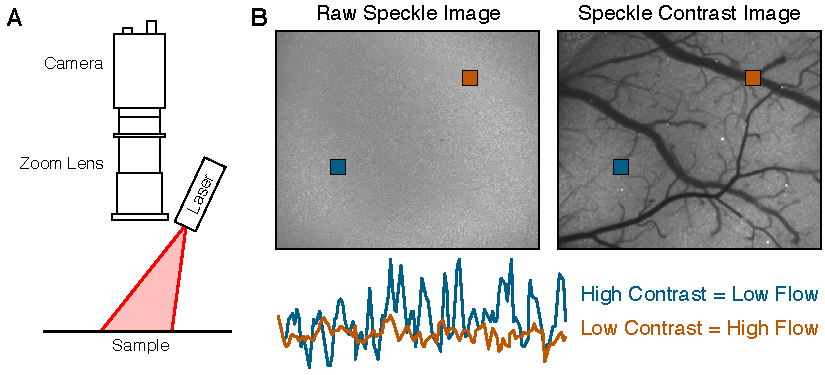
\includegraphics{figures/chapter_1/lsci_schematic.pdf}
    \caption{
        \label{fig:lsci_schematic}
        \textbf{(A)} Traditional LSCI microscope system consisting of an illuminating laser, imaging optics, and a camera. \textbf{(B)} Raw intensity image of the speckle pattern and the resulting speckle contrast image from vasculature in the mouse cerebral cortex. Regions of high contrast in the intensity image (blue) have low flow compared to regions with low contrast (orange), which have high flow.
    }
\end{figure}

An example of the raw intensity image of the speckle pattern and corresponding computed speckle contrast image are shown in Figure \ref{fig:lsci_schematic}B. The imagery was obtained \textit{in vivo} from the cerebral cortex of a mouse under general anesthesia. The graininess of the speckle pattern can be seen in the raw intensity image, with some regions appearing more blurred than others. The speckle contrast image was computed directly from the intensity image using Equation \ref{eq:speckle_contrast} to generate a two-dimensional map of motion for the field-of-view. Within the cortex, erythrocytes are the primary moving scattering particles and therefore vasculature is highlighted by the speckle contrast image. Regions of higher flow, such as a large vessel, experience more blurring of the speckle pattern and therefore have lower $K$ values. Conversely, regions of low flow, such as the space between resolvable surface vessels (parenchyma), experience less blurring and therefore have higher $K$ values. Measurements within the parenchyma sample the slower, more isotropic blood flow of unresolvable microvasculature beneath the surface of the cortex.

The shallow depth penetration of LSCI is a significant limitation of the imaging technique. Detected photons only sample a few hundred microns of superficial tissue without any depth resolution and are heavily-weighted towards large surface vasculature \cite{Davis:2014kc}. While skin and retinal imaging can be performed directly on the tissue of interest, CBF imaging requires either thinning or removing the skull to gain optical access \cite{Boas:2010vr}.

%%%%%%%%%%%%%%%%%%%%%%%%%%%%%%%%%%%%%%%%%%%%%%%%%%%%%%%%%%%%%%%%%%%%%%%%%%%%%%%
\subsubsection{Instrumentation}

The simple instrumentation necessary to perform LSCI has contributed to its popularity as a blood flow imaging technique. A basic LSCI microscope consists of an illuminating laser, imaging optics, and a camera (Figure \ref{fig:lsci_schematic}A). The laser output is expanded to broadly epi-illuminate the area of interest at a normal to oblique angle depending on the application. Red to near-infrared laser diodes (600-850 nm) are typically used to take advantage of the tissue optical window where scattering dominates absorption by hemoglobin or water. Because LSCI is based entirely upon scattering, wavelength is less important than other imaging techniques that rely upon absorption. However, the coherence length of the laser dictates the longest possible path length through the tissue that can be properly sampled for quantitative flow information. Lasers with narrow spectral bandwidths (e.g. single longitudinal mode or narrow linewidth lasers) offer coherence lengths of several meters and are more than sufficient for use in LSCI.

Camera selection varies broadly in literature and generally any charge-coupled device (CCD) or complementary metal-oxide-semiconductor (CMOS) camera is appropriate for use with LSCI \cite{Draijer:2008ic, Boas:2010vr}. Even cheap cameras such as webcams have been shown to provide reliable blood flow imagery \cite{Richards:2013bi}. While spectral sensitivity, bit depth, pixel size, frame rate, and noise are all important factors to consider, most researchers use the cameras readily available in their laboratories. However, it is critical that the speckle pattern is properly sampled such that the speckle size is at least twice the size of a single camera pixel \cite{Kirkpatrick:2008ke}. Deviation from the spatial Nyquist sampling criterion will reduce contrast and decrease the variation in the speckle contrast image.

%%%%%%%%%%%%%%%%%%%%%%%%%%%%%%%%%%%%%%%%%%%%%%%%%%%%%%%%%%%%%%%%%%%%%%%%%%%%%%%
\subsubsection{Quantitative Accuracy}

Speckle contrast values are only indicative of the amount of motion in a sample and are not linearly proportional to particle speed or volumetric flow. Understanding the nonlinear relationship with the complex underlying blood flow is an active area of research in the DLS field \cite{Duncan:2008fd, Briers:2013es}. Quantitative flow measurements require accurately relating the speckle contrast value to the characteristic decay time ($\tau_c$) of the speckle autocorrelation function. DLS theory has established that the speckle autocorrelation time is inversely proportional to the speed of the scatters in the single scattering regime \cite{Bonner:1981hga} and weighted by the number of dynamic scattering events under multiple scattering \cite{Boas:1997kf, Kazmi:2015du, Davis:2016ik}. Since Fercher and Briers first proposed a simple model relating $K$ and $\tau_c$ \cite{Fercher:1981jh}, there have been numerous improvements to more robustly extract the flow contributions from the observed speckle \cite{Bandyopadhyay:2005bg, Parthasarathy:2008el}. The model described by Bandyopadhyay \textit{et al.} \cite{Bandyopadhyay:2005bg} relates the measured $K$ with $\tau_c$:
%
% Equation - Bandyopadhyay Equation
\begin{equation}
    \label{eq:bandyopadhyay}
    K(T,\tau_c) = \left(\beta \frac{e^{-2x} - 1 + 2x}{2x^{2}}\right)^{1/2}
\end{equation}
%
where $x = T/\tau_c$, $T$ is the camera exposure time, and $\beta$ is a normalization factor that accounts for speckle averaging due to the mismatch between speckle size and pixel size, polarization, and the finite coherence length of the laser \cite{Lemieux:1999ko}. $\beta$ is frequently assumed to be equal to 1, limiting the technique to relative measures of flow. This model assumes that detected photons only experience single scattering interactions and that the underlying particle motion has a Lorentzian velocity distribution. Despite these assumptions, Equation \ref{eq:bandyopadhyay} has been used extensively to relate measured speckle contrast with relative blood flow \cite{Dunn:2011gi,Boas:2010vr} and will be used throughout this dissertation.

The inverse correlation time (ICT) is frequently interpreted as being proportional to the speed of the moving particles ($1/\tau_c \propto \nu_{scatterers}$) based on assumptions from laser Doppler flowmetry \cite{Bonner:1981hga}. While highly dependent upon the optical properties and flow conditions of the sample, ICT values in single vessels correspond to the speed of the flowing erythrocytes. In parenchyma regions, ICT is a measure of local perfusion because flow cannot be isolated to individual vessels from the depth integrated contributions of the unresolvable microvasculature \cite{Durduran:2016el, Dunn:2011gi}. Despite these assumptions and limitations, multiple studies have demonstrated strong correlations between LSCI estimates of CBF and absolute measurements from other perfusion indices \cite{Ayata:2004ba, Strong:2005kj, Kazmi:2015du}. The development of multi-exposure speckle imaging \cite{Parthasarathy:2008el} has improved the quantitative accuracy of the LSCI technique and will be discussed extensively in Chapter \ref{ch:mesi}.



%%%%%%%%%%%%%%%%%%%%%%%%%%%%%%%%%%%%%%%%%%%%%%%%%%%%%%%%%%%%%%%%%%%%%%%%%%%%%%%
% Section 1.3 - Measuring Oxygen Tension In Vivo
%%%%%%%%%%%%%%%%%%%%%%%%%%%%%%%%%%%%%%%%%%%%%%%%%%%%%%%%%%%%%%%%%%%%%%%%%%%%%%%
\section{Measuring Oxygen Tension \textit{In Vivo}}

\textit{In vivo} measurements of molecular oxygen have historically been made using highly invasive Clarke electrodes that are limited to point measurements outside the vascular lumen \cite{Vovenko:1999be, Tsai:2003cc, Roussakis:2015eu}. While targets as small as a few microns can be measured with the appropriate electrode, there are significant tradeoffs between the signal-to-noise ratio and spatial specificity depending on probe size. Electrodes can also only approximate intravascular oxygen concentrations through measurements in nearby interstitial tissue. Magnetic resonance techniques allow for noninvasive imaging of hemoglobin saturation, but suffer from low spatial resolutions and can only be correlated with free oxygen levels in the blood \cite{Roussakis:2015eu, Dunn:2003hg, Hou:2003hb, Liu:2006bt}. Oxygen-sensitive porphyrin probes allow for noninvasive, highly sensitive optical oxygenation measurements based on phosphorescence quenching \cite{Vinogradov:2012tda}. While an injection of the probe is required, absolute oxygen tension (\ce{pO2}) can be directly calculated from the lifetime of the measured phosphorescence decay.

%%%%%%%%%%%%%%%%%%%%%%%%%%%%%%%%%%%%%%%%%%%%%%%%%%%%%%%%%%%%%%%%%%%%%%%%%%%%%%%

\subsection{Oxygen-Dependent Quenching of Phosphorescence}
Recent advances in oxygen-sensitive probe design have made oxygen-dependent quenching of phosphorescence a powerful tool for \textit{in vivo} measurements of \ce{pO2} within both intravascular and interstitial spaces \cite{Vinogradov:2012tda, Esipova:2011hi}. This method relies upon dissolved environmental oxygen quenching the phosphorescence of porphyrin dyes or ruthenium complexes, which causes a change in excited state lifetime (Figure \ref{fig:jablonski}A).  The \ce{pO2} can be quantified from the measured lifetime (Appendix \ref{app:stern_volmer}) using the Stern-Volmer relationship:
%
% Equation - Stern-Volmer Relationship
\begin{equation}
    \label{eq:stern-volmer}
    \frac{\tau_{0}}{\tau} = 1 + k_{q}\tau_{0}[pO_{2}]
\end{equation}
%
where $\tau$ is the measured phosphorescence lifetime, $\tau_{0}$ is the unquenched lifetime, and $k_{q}$ is a probe-specific quenching rate constant that depends upon the local environment (temperature, pH, atmospheric pressure, and salinity). Equation \ref{eq:stern-volmer} allows for the absolute \ce{pO2} to be obtained from the measured phosphorescence lifetime provided $k_q$ and $\tau_{0}$ are well-characterized under physiological conditions. Furthermore, because lifetime measurements are independent of absolute intensity, they can easily be isolated from other chromophores and tissue scattering, making them ideal for integration into multi-modal imaging systems.

% Figure - Jablonksi Diagram
\begin{figure}
    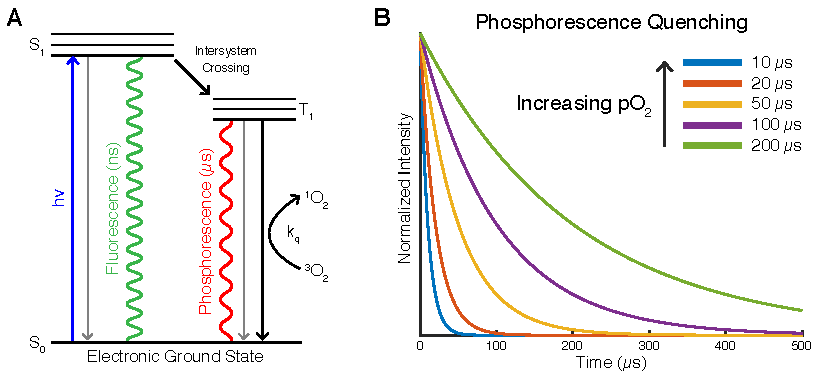
\includegraphics{figures/chapter_1/jablonski.pdf}
    \caption{
        \label{fig:jablonski}
        \textbf{(A)} Jablonski diagram of phosphorescence quenching by environmental molecular oxygen. \textbf{(B)} Phosphorescence quenching causes a reduction in the measured lifetime and is dependent upon [\ce{O2}] or \ce{pO2}.
    }
\end{figure}

The phosphorescence lifetime can be measured in the time domain by exciting the probe with a short pulse of light and collecting the emitted phosphorescence. The resulting phosphorescent decay curve can then be fit to an exponential to obtain the phosphorescence lifetime ($\tau$):
%
% Equation - Exponential Decay
\begin{equation}
    \label{eq:exponential_decay}
    I(t) = A + Be^{-t / \tau}
\end{equation}

Alternatively, frequency domain measurements can be made by calculating the phase shift or demodulation of the phosphorescence generated by sinusoidally-modulated light. While excitation light is utilized more efficiently in frequency domain measurements, they are more difficult to implement and process than time domain measurements.

Point detectors such as avalanche photodiodes or photomultiplier tubes are commonly used to acquire the phosphorescent decays because of their high sensitivity, gain, and temporal resolutions. However, these detectors limit the lifetime measurements to single spatial locations unless laser scanning systems \cite{Yaseen:2009ep, Kazmi:2013ey} or intensified exposure-gated cameras \cite{Shonat:2003ia, Sakadzic:2009jo} are utilized. Despite these limitations, \textit{in vivo} measurements of oxygen-dependent quenching of phosphorescence have been conducted in a variety of tissues including the retina, brain, muscle, and peritoneum \cite{Vovenko:1999be}. The technique has also been used extensively to study cortical oxygenation, often in conjunction with other imaging modalities \cite{Yu:2013fd, Devor:2014ke}.



%%%%%%%%%%%%%%%%%%%%%%%%%%%%%%%%%%%%%%%%%%%%%%%%%%%%%%%%%%%%%%%%%%%%%%%%%%%%%%%
% Section 1.4 - Research Overview
%%%%%%%%%%%%%%%%%%%%%%%%%%%%%%%%%%%%%%%%%%%%%%%%%%%%%%%%%%%%%%%%%%%%%%%%%%%%%%%
\section{Research Overview}

The overall goal of this project is the development of an optical imaging platform capable of the chronic monitoring of cortical hemodynamics during ischemic stroke and the subsequent recovery. The system combines two different imaging techniques, LSCI and oxygen-dependent quenching of phosphorescence, to measure CBF and \ce{pO2} within cortical vasculature. The development of the imaging system has four iterative milestones, each extending the capabilities of the platform. Chapter \ref{ch:system} details the initial design and construction of the dual-modality system and demonstrates acute \textit{in vivo} measurements in mice. Chapter \ref{ch:photothrombosis} describes modifications to the system to perform artery-targeted photothrombosis, an extension of the conventional photothrombotic model of ischemic stroke. The technique is demonstrated \textit{in vivo} with the acute and chronic hemodynamics monitored using the imaging platform. The functional effects of the targeted infarct on fine motor skills are also examined. Chapter \ref{ch:mesi} details the implementation of multi-exposure speckle imaging to improve the robustness of chronic CBF measurements. Finally, Chapter \ref{ch:awake} describes the transition to awake animal imaging and demonstrates chronic imaging of the recovery from targeted photothrombotic stroke.



%%%%%%%%%%%%%%%%%%%%%%%%%%%%%%%%%%%%%%%%%%%%%%%%%%%%%%%%%%%%%%%%%%%%%%%%%%%%%%%
% END Chapter 1
%%%%%%%%%%%%%%%%%%%%%%%%%%%%%%%%%%%%%%%%%%%%%%%%%%%%%%%%%%%%%%%%%%%%%%%%%%%%%%%


% Chapter 2 - Simultaneous Imaging of Cerebral Blood Flow and Oxygen Tension
%%%%%%%%%%%%%%%%%%%%%%%%%%%%%%%%%%%%%%%%%%%%%%%%%%%%%%%%%%%%%%%%%%%%%%%%%%%%%%%
% Chapter 2 - Simultaneous Imaging of Cerebral Blood Flow and Oxygen Tension
%%%%%%%%%%%%%%%%%%%%%%%%%%%%%%%%%%%%%%%%%%%%%%%%%%%%%%%%%%%%%%%%%%%%%%%%%%%%%%%

\chapter{Simultaneous Imaging of Cerebral Blood Flow and Oxygen Tension} \label{ch:system}

Measurements of hemodynamic parameters in cerebral vasculature have been invaluable in preclinical research for understanding the physiology of the normal and diseased brain. The combination of imaging techniques to simultaneously measure multiple hemodynamic parameters has become increasingly common and used to study stroke \cite{Jones:2008gb}, cortical spreading depression \cite{Sakadzic:2009jo}, and functional brain activation \cite{Dunn:2005gw, Dunn:2003wy}. Advancements in computer processing power and the increased availability of lasers and light-emitting diodes across a diverse range of wavelengths have facilitated the development of these multi-parameter hemodynamic imaging platforms.

In 2010, Ponticorvo and Dunn \cite{Ponticorvo:2010uv} detailed a dual-modality imaging system capable of simultaneously measuring cerebral blood flow (CBF) and oxygen tension (\ce{pO2}) in cortical vasculature. The system combined laser speckle contrast imaging (LSCI) and oxygen-dependent quenching of phosphorescence. An unpublished modification to the system added multispectral reflectance imaging for measurements of oxy- and deoxyhemoglobin \cite{Ponticorvo:2010ur}. The primary innovation of this design was the use of a digital micromirror device (DMD) to achieve spatial localization of the phosphorescent signal. A DMD is an optical semiconductor device that consists of a two-dimensional array of thousands of individually addressable mirrors that can be tilted to spatially modulate light. By patterning excitation light, phosphorescence could be constrained to only the targeted regions of interest, which allowed the use of high sensitivity point detectors. This overcame the traditional limitations of spatially-resolved phosphorescence imaging that either required the use of expensive laser scanning systems \cite{Yaseen:2009ep, Kazmi:2013ey} or exposure-gated cameras \cite{Shonat:2003ia, Sakadzic:2009jo}.

However, a major limitation of this system was the phosphorescent probe Oxyphor R2 \cite{Dunphy:2002tz}, which required conjugation with albumin in order to remain stable \textit{in vivo}. The system was also optically limited to only targeting large regions of the field of view (FOV) for \ce{pO2} measurements and was incapable of performing multiple actions simultaneously with the DMD. This chapter details a redesign of the system by Ponticorvo and Dunn \cite{Ponticorvo:2010uv} with the goal of improving the spatial and temporal resolutions of both imaging modalities through implementation of newer hardware and a more robust oxygen-sensitive phosphorescent probe.



%%%%%%%%%%%%%%%%%%%%%%%%%%%%%%%%%%%%%%%%%%%%%%%%%%%%%%%%%%%%%%%%%%%%%%%%%%%%%%%
% Section 2.1 - Instrumentation
%%%%%%%%%%%%%%%%%%%%%%%%%%%%%%%%%%%%%%%%%%%%%%%%%%%%%%%%%%%%%%%%%%%%%%%%%%%%%%%
\section{Instrumentation}

The following dual-modality imaging system combines LSCI with oxygen-dependent quenching of phosphorescence for the simultaneous measurement of CBF and \ce{pO2}. Because LSCI is rarely light-limited, the optical design is focused on the projection of patterned excitation light off the DMD and the efficient collection of the emitted phosphorescence. The spectral cutoffs for the system were dictated by the new phosphorescent probe, Oxyphor PtG4 \cite{Esipova:2011hi}, an oxygen-sensitive dendritic probe that contains Platinum(II)-\textit{meso}-tetra-(3,5-dicarboxyphenyl)tetrabenzoporphyrin (PtTBP) as the phosphorescent core.

% Figure - Oxyphor PtG4 Spectra + Calibration
\begin{figure}
    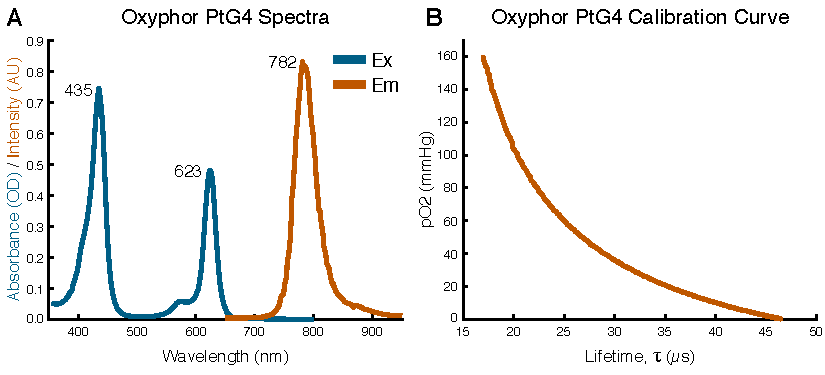
\includegraphics{figures/chapter_2/oxyphorptg4.pdf}
    \caption{
        \label{fig:oxyphor_ptg4}
        \textbf{(A)} Excitation (blue) and emission (red) spectra for Oxyphor PtG4. \textbf{(B)} Calibration curve relating environmental \ce{pO2} to the measured phosphorescence lifetime ($\tau$) under physiological conditions (37 $^\circ$C, pH 7.2).
    }
\end{figure}

Unlike its predecessors Oxyphor R2 and G2 \cite{Dunphy:2002tz}, which were limited to albumin-rich environments for stability, Oxyphor PtG4 is encapsulated within a hydrophobic dendrimer and PEGylated to increase solubility and biocompatibility. These modifications provide increased stability across a wider range of temperatures and pH values and eliminate the need for conjugation with blood proteins \cite{Esipova:2011hi}. Oxyphor PtG4 has two excitation maxima near 435 nm (Soret) and 623 nm (Q band) and a broad emission spectra peaking at 782 nm (Figure \ref{fig:oxyphor_ptg4}A). The probe was calibrated under physiological conditions (37 $^\circ$C, pH 7.2) by measuring the phosphorescent decay lifetime ($\tau$) as the environmental \ce{pO2} was increased from 0 mmHg to 160 mmHg (Figure \ref{fig:oxyphor_ptg4}B). The unquenched lifetime ($\tau_0$) is 47 $\mu$s in an oxygen-free environment.

%%%%%%%%%%%%%%%%%%%%%%%%%%%%%%%%%%%%%%%%%%%%%%%%%%%%%%%%%%%%%%%%%%%%%%%%%%%%%%%
\subsection{Optical System}

The schematic of the optical system can be seen in Figure \ref{fig:systemschematic_1}. The excitation and emission spectra of Oxyphor PtG4 dictated laser selection and dichroic beamsplitter cutoff wavelengths. LSCI was performed using a 685 nm laser diode (50 mW, HL6750MG, Thorlabs, Inc.) illuminating the sample at an oblique angle. The laser was mounted in a temperature-controlled housing (TCLDM9, Thorlabs, Inc.) and collimated with a slight divergence using an aspheric lens (C240TME-B, Thorlabs, Inc.) to illuminate the entire FOV. The operating current was set using a laser diode controller (LDC202, Thorlabs, Inc.) and the diode temperature regulated using a temperature controller (TED200C, Thorlabs, Inc.). The scattered light was relayed through a pair of dichroic beamsplitters and a bandpass filter (685$\pm$40 nm, S685/40m, Chroma Technology Corp.) to an NIR-enhanced CMOS camera (acA1300-60gmNIR, 1280 x 1024 pixels, Basler AG) with 2x magnification for a FOV of 3.5 x 2.8 mm. The camera was controlled via the Basler Pylon API using custom software written in C++ (i.e. the "Speckle Software").

% Figure - System Schematic (Ver. 1)
\begin{figure}
    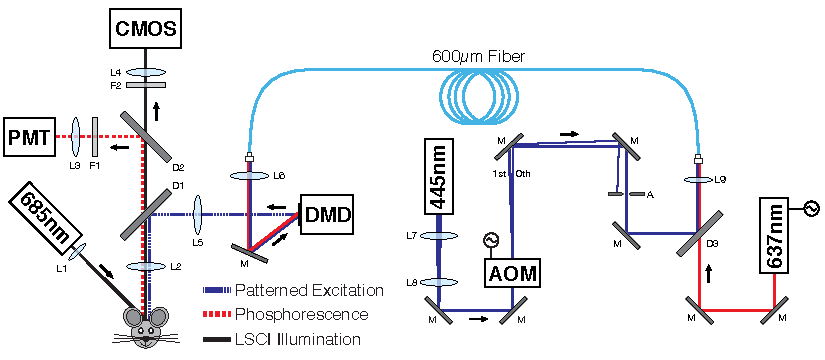
\includegraphics{figures/chapter_2/systemschematic.pdf}
    \caption{
        \label{fig:systemschematic_1}
        Schematic of the dual-modality imaging system combining LSCI with oxygen-dependent quenching of phosphorescence.
    }
\end{figure}

Separately, two different lasers at 445 nm and 637 nm were selected to target the Soret and Q band excitation maxima of Oxyphor PtG4. Each laser can be used independently to collect phosphorescence lifetime measurements with different penetration depths and sample volumes because of their wavelengths. The 445 nm laser (200 mW, AixiZ) is a packaged device with a 4 mm collimated output that operates at a fixed current with convection cooling. The beam size was reduced to 1 mm and gated using an 80 MHz acousto-optic modulator (23080-2-LTD AOM and 21080-1AM RF Driver, Neos Technologies, Inc.). The 637 nm laser diode (250 mW, HL6388MG, Thorlabs, Inc.) was mounted in a temperature-controlled housing (LDM21, Thorlabs, Inc.) and collimated using an aspheric lens (C330TME-B, Thorlabs, Inc.). The laser was directly gated using its driver (LDD400-1P, Wavelength Electronics, Inc.) and the diode temperature regulated using an external temperature controller (300B, Newport Corp.). Both lasers were gated via analog modulation to produce 20 $\mu$s pulses of light for time domain lifetime measurements.

The lasers were coaligned using a red hot mirror (580 nm cutoff, FM02, Thorlabs, Inc.) and coupled into a fiber optic patch cord (P600-2-VIS-NIR, Ocean Optics, Inc.) with a 600 $\mu$m core size. The modulated laser light was relayed to the primary imaging system via the patch cord and re-collimated to illuminate the DMD. A DLP LightCrafter Evaluation Module (Texas Instruments) was modified to expose the bare DMD (DLP3000, 608 x 684 pixels, 7.6 $\mu$m pitch, Texas Instruments) for illumination. The spatially patterned modulated light was then relayed to the sample with 0.5x magnification to selectively excite Oxyphor PtG4 for lifetime measurements.

The emitted phosphorescence was separated from the excitation and scattered LSCI laser light using a pair of dichroic beamsplitters (650 nm, ZT640rdc, Chroma Technology and 750 nm, FF750-SDi02, Semrock, Inc.) and a bandpass filter (810$\pm$90 nm, ET810/90m, Chroma Technology Corp.) and relayed to a photomultiplier tube for detection (H7422P-50, Hamamatsu Photonics K.K.). Figure \ref{fig:systemspectra} contains an overview of the spectral separation in the imaging system and Table \ref{tab:filters} details each filter in the primary imaging path.

% Figure - System Spectra
\begin{figure}
    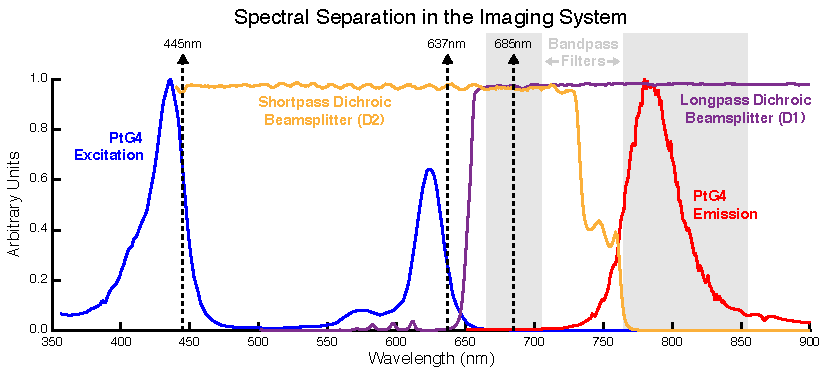
\includegraphics{figures/chapter_2/systemspectra.pdf}
    \caption{
        \label{fig:systemspectra}
        Dichroic beamsplitters and bandpass filters used to spectrally separate light in the imaging system. A longpass dichroic beamsplitter (purple) separates the excitation lasers (445 and 637 nm) from the scattered LSCI laser (685 nm) and Oxyphor PtG4 phosphorescence emission (red). A shortpass dichroic beamsplitter (gold) separates the LSCI light from the phosphorescence for detection. Bandpass filters (shaded grey) limit ambient and scattered light from reaching the detectors. All values are normalized.
    }
\end{figure}

% Table - Filter Summary
\begin{table}
    \caption{Summary of optical filters in the imaging system.}
    \label{tab:filters}
    \centering
    \resizebox{\textwidth}{!}{
    \begin{tabular}{ccccc} \addlinespace \toprule
        \thead{Label} & \thead{Filter} & \thead{Usage} & \thead{Manufacturer} & \thead{Part Number} \\ \midrule
        \textbf{D1} & \makecell{650 nm longpass \\ dichroic beamsplitter} & \makecell{Excitation \\ Separation} & Chroma & ZT640rdc \\ \hline
        \textbf{D2} & \makecell{750 nm shortpass \\ dichroic beamsplitter} & \makecell{Emission \\ Separation} & Semrock & FF750-SDi02-25x36 \\ \hline
        \textbf{D3} & \makecell{580 nm red hot mirror} & \makecell{Laser \\ Coalignment} & Thorlabs & FM02 \\ \hline
        \textbf{F1} & \makecell{810$\pm$90 nm \\ bandpass} & \makecell{Phosphorescence \\ Isolation} & Chroma & ET810/90m \\ \hline
        \textbf{F2} & \makecell{685$\pm$40 nm \\ bandpass} & \makecell{LSCI \\ Isolation} & Chroma & S685/40m \\ \bottomrule
    \end{tabular}}
\end{table}

%%%%%%%%%%%%%%%%%%%%%%%%%%%%%%%%%%%%%%%%%%%%%%%%%%%%%%%%%%%%%%%%%%%%%%%%%%%%%%%
\subsection{Acquisition Control} \label{ssec:acquisition_control}

An overview of the control system can be seen in Figure \ref{fig:controlschematic}. Both LSCI and the phosphorescence lifetime measurements were performed simultaneously using a single computer. The LSCI acquisition is controlled via the Speckle Software, which implements the Basler Pylon API for comprehensive control of the GigE camera. The Speckle Software allows for the real-time calculation, display, and writing of speckle contrast imagery using an efficient processing algorithm \cite{Tom:2008tg}. The camera was operated with a 5 ms exposure time, which is standard for \textit{in vivo} microvasculature studies using LSCI \cite{Yuan:2005tj}. Raw intensity images were acquired in bursts and saved at an effective 60 frames per second (fps) at an 8-bit bit depth. The computed speckle contrast images were saved as single-precision floating-point numbers and averaged together ($n$ = 45 frames) during post-processing for a final frame rate of 1.33 fps. A standard LSCI acquisition produced data at a rate of 55 MB/s.

% Figure - System Control Schematic
\begin{figure}
    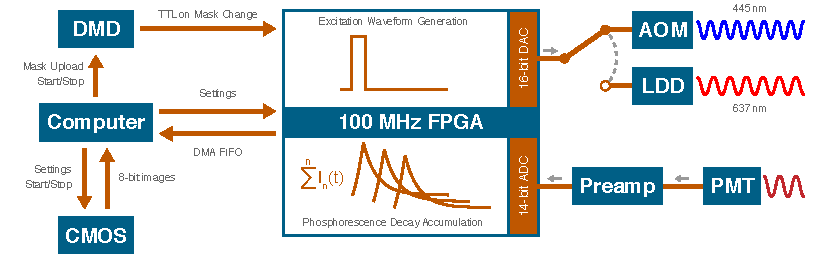
\includegraphics{figures/chapter_2/controlschematic.pdf}
    \caption{
        \label{fig:controlschematic}
        Imaging system control schematic. The phosphorescence excitation waveform can be sent to either the AOM for modulating the 445 nm laser or the LDD for modulation the 637 nm laser.
    }
\end{figure}

The Speckle Speckle software was also modified to control the DMD via its Ethernet-over-USB command interface. Users can define arbitrarily-shaped regions of interest (ROIs) using the LSCI camera as reference and upload the resulting binary masks to the DMD for the patterning of excitation light. Registration between the camera and the projected pattern can be performed using the Speckle Software to guarantee alignment with the reference image (see Section \ref{ssec:dmd_registration}). Individual patterns or timed pattern sequences can be uploaded and displayed on the DMD, with a TTL pulse emitted on each pattern change.

While the Speckle Software controls the patterning of excitation light for the lifetime measurements, a separate LabVIEW (National Instruments Corp.) program controls the waveform generation and phosphorescence decay acquisition. A field-programmable gate array (FPGA) operating on a single-cycle timed loop oversees digital-to-analog (DAC) and analog-to-digital (ADC) conversion. The FlexRIO FPGA (PXIe-7965R, National Instruments Corp.) and 100 MHz transceiver module (NI-5781, National Instruments Corp.) reside in a PXI chassis (PXIe-1082, National Instruments Corp.) with a high-bandwidth embedded controller (PXIe-8130, National Instruments Corp.). The FPGA communicates with the host computer over a 1 Gigabit Ethernet connection.

Waveform generation and acquisition occur simultaneously on the FPGA with each complete cycle taking 32,768 ticks at the 100 MHz clock rate. Each cycle is triggered upon DMD pattern change via TTL through an auxiliary input on the transceiver. The excitation waveform contains a 20 $\mu$s square pulse (2,000 ticks) for an overall 6\% duty cycle and is output from the transceiver DAC between 0-1 V. Minimizing the pulse duration and duty cycle were important because high excitation flux levels can produce damaging levels of singlet oxygen \cite{Wilson:2005te}. If the 445 nm laser is being used, then the analog signal is directed into the AOM. If the 637 nm laser is being used, then the output is inverted and connected to the laser diode driver. The resulting phosphorescence is detected by the PMT and amplified at a fixed 50 mV/$\mu$A gain at 10 MHz (C9999, Hamamatsu Photonics K.K.). The analog signal is digitized by the transceiver ADC with a 14-bit depth resolution. In order to reduce the amount of data being saved, the FPGA accumulates the sum of $n$ cycles of phosphorescent decays before transferring to the host computer via a direct memory access (DMA) FIFO buffer. The LabVIEW program writes the accumulated phosphorescent signal to a binary file (32-bit integer) for post-processing. An optional setting enables on-the-fly fitting of the phosphorescence decay curve for $\tau$ and estimates the \ce{pO2} using the Oxyphor PtG4 calibration curve. However, this added computation can result in DMA FIFO overflow at higher acquisition speeds.

% Table - Lifetime Measurement Settings
\begin{table}
    \caption[Common phosphorescence lifetime acquisition settings]{
        Common acquisition settings for the phosphorescence lifetime measurements ($n$ = number of DMD patterns). Raw data is acquired by the FPGA at a rate of 160 MB/s.
    }
    \label{tab:lifetime_settings}
    \centering
    \resizebox{\textwidth}{!}{
    \begin{tabular}{cccc} \addlinespace \toprule
        \thead{\makecell{Pattern Rate \\ (Hz)}} & \thead{\makecell{Decays Accumulated \\ (per Pattern)}} & \thead{\makecell{Temporal \\ Resolution (s)}} & \thead{\makecell{Host Data \\ Rate (KB/s)}} \\ \midrule
        1 & 2500 & $n$ & 64 \\ \hline
        2 & 1250 & $n/2$ & 128 \\ \hline
        10 & 250 & $n/10$ & 640 \\ \hline
        50 & 50 & $n/50$ & 3200 \\ \hline
        100 & 25 & $n/100$ & 6400 \\ \bottomrule
    \end{tabular}}
\end{table}

Unlike LSCI, which operates at a fixed frame rate, the temporal resolution of the phosphorescence lifetime measurements is linearly dependent upon the number of patterns being displayed on the DMD and the number of decays accumulated on the FPGA. The digital controller on the DLP LightCrafter can store 96 binary patterns on its internal memory buffer and operate at a maximum pattern rate of 4000 Hz. The number of decays to accumulate on the FPGA is ultimately determined by the strength of the phosphorescent signal, which is influenced by the projected pattern size, Oxyphor PtG4 concentration, and laser power. The amount of data transferred to the host computer is inversely proportional to the number of records accumulated. Table \ref{tab:lifetime_settings} details several acquisition settings for the phosphorescence lifetime measurements with the 2 and 10 Hz pattern rates most commonly being utilized. While higher pattern rates offer higher temporal resolutions, the reduced averaging of the phosphorescent decays negatively affects the quality of the lifetime fitting.

A summary of the acquisition timing can be seen in Figure \ref{fig:timingschematic} with both LSCI and the phosphorescence lifetime measurements operating simultaneously but independently. This is possible because of the spectral separation of the excitation and emission wavelengths (Figure \ref{fig:systemspectra}). Both imaging modalities share the same computer clock, so timestamps can easily be aligned during post-processing.

% Figure - Acquisition Timing
\begin{figure}
    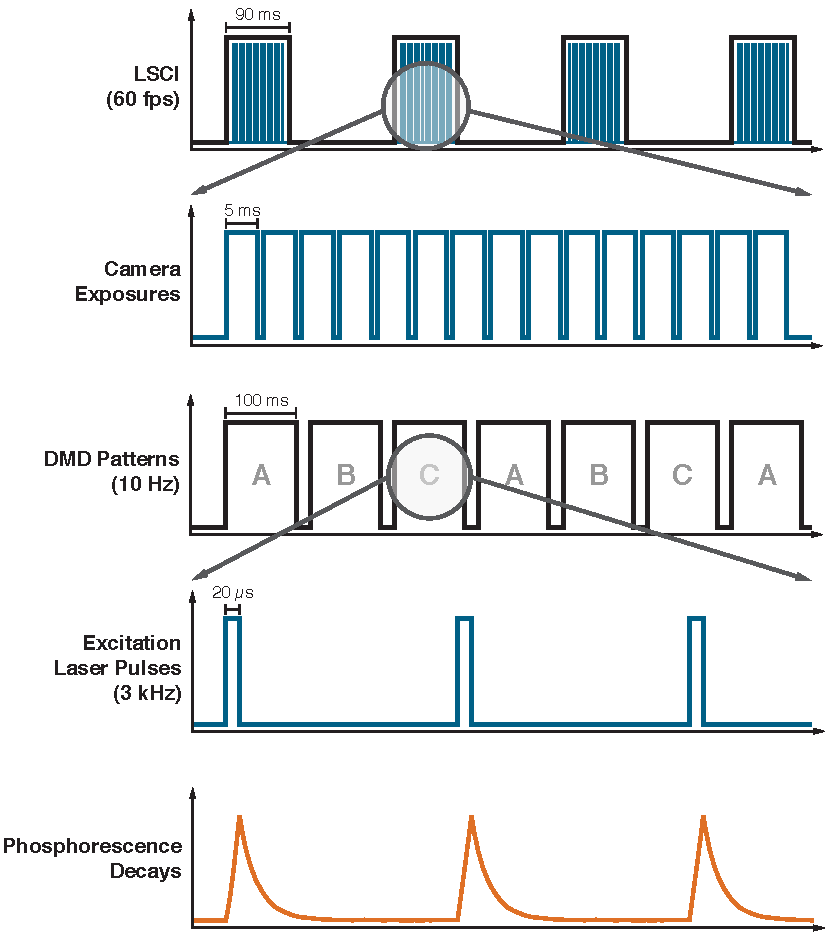
\includegraphics{figures/chapter_2/timingschematic.pdf}
    \caption{
        \label{fig:timingschematic}
        Acquisition timing paradigm for the LSCI and phosphorescence lifetime measurements.
    }
\end{figure}

%%%%%%%%%%%%%%%%%%%%%%%%%%%%%%%%%%%%%%%%%%%%%%%%%%%%%%%%%%%%%%%%%%%%%%%%%%%%%%%
\subsubsection{Troubleshooting}

During development of the phosphorescence lifetime measurement system, two significant problems were encountered. The first was a severe bandwidth limitation in the original preamplifier (SR570, Stanford Research Systems) used to convert the current output from the PMT to a voltage signal for ADC. The preamplifier was operated in “high bandwidth” mode with no filters active and a gain of 50 mV/$\mu$A. This corresponds to a bandwidth between 200-800 kHz. The maximum possible bandwidth is 1 MHz and can only be achieved at the lowest gain setting. This bandwidth is insufficient to properly sample the phosphorescent decay curve at higher \ce{pO2} levels as $\tau$ grows exponentially shorter (Figure \ref{fig:oxyphor_ptg4}B). The limitation was identified while performing measurements under ambient conditions where \ce{pO2} \textgreater 150 mmHg. At this \ce{pO2} level, a 1 $\mu$s change in $\tau$ corresponds to over a 20 mmHg change in \ce{pO2}. The problem was resolved by transitioning to the higher bandwidth (10 MHz) preamplifier detailed in Section \ref{ssec:acquisition_control}. The \textgreater 10x increase in bandwidth allows for proper sampling of the entire physiologically-relevant portion of the Oxyphor PtG4 calibration curve.

The second issue was related to the clock settings for the single-cycle timed loop on the FPGA. The PXIe-7965 FPGA module offers an onboard 40 MHz clock that was selected by default as the clock for the timed loop. However, this requires crossing clock domains from the 100 MHz sample clock on the NI-5781 transceiver to the onboard clock of the FPGA module. This can result in data corruption because the FPGA can capture data as it is actively being updated at the higher sample rate. In order to safely cross clock domains while guaranteeing data integrity, a FIFO buffer must be implemented. Alternatively, the sample clock on the transceiver module can be used as the clock for the single-cycle timed loop, which is how the issue was resolved on this system. Operating at 100 MHz does result in oversampling our expected signal, which is a problem that could be resolved by discarding unwanted samples.

%%%%%%%%%%%%%%%%%%%%%%%%%%%%%%%%%%%%%%%%%%%%%%%%%%%%%%%%%%%%%%%%%%%%%%%%%%%%%%%
\subsection{DMD Alignment and Registration} \label{ssec:dmd_registration}

Proper alignment and illumination of the DMD is critical for accurately projecting the excitation light patterns. The DLP3000 DMD contains a 0.3-inch diagonal micromirror array with 608 x 684 pixels arranged in a diamond configuration with a $\pm$12$^\circ$ tilt angle (Figure \ref{fig:dmdmirror}A). The DMD must be illuminated at -24$^\circ$ from the normal for the specularly reflected light from mirrors in the ON position to be directed along the desired optical axis (Figure \ref{fig:dmdmirror}B). Light reflected from pixels in the OFF position will be directed +48$^\circ$ off axis and can easily be blocked.

Because coherent light is being utilized, diffraction off the two-dimensional (2D) micromirror array must be considered. The physics are analogous to that of a 2D diffraction grating, except that two separate diffraction patterns will be formed, each influenced by the two possible mirror positions (Figure \ref{fig:dmdmirror}C). The position of the $(0,0)$ order and the intensity envelope follows the specular reflection off the tilted mirror as described above. However, all other orders are dependent upon incident angle, mirror pitch, mirror angle, and wavelength \cite{TexasInstruments:2009tr}. Isolating light from an single order at a specific wavelength requires adjusting the incident angle until the intensity envelope is aligned with the desired order. This will result in the outbound light no longer being normal to the face of the DMD, which can complicate downstream alignment. Alternatively, the diffracted light can be collimated and focused onto to the desired projection location using a pair of lenses. This effectively images the face of the DMD to the sample plane using the same alignment procedure as incoherent light.

% Figure - DMD Mirror Explanation
\begin{figure}
    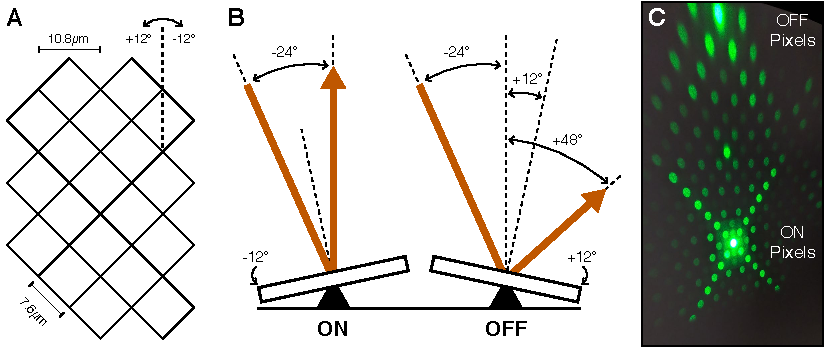
\includegraphics{figures/chapter_2/dmdmirror.pdf}
    \caption{
        \label{fig:dmdmirror}
        \textbf{(A)} Mirrors are arranged in a diamond configuration on the DMD with a 7.6 $\mu$m pitch and a $\pm$12$^\circ$ tilt angle. \textbf{(B)} Mirrors in the ON position will direct incident light perpendicular to the face of the DMD while mirrors in the OFF state will direct light off axis. \textbf{(C)} Diffraction patterns produced by coherent light illuminating the DMD.
    }
\end{figure}

% Figure - DMD Alignment
\begin{figure}
    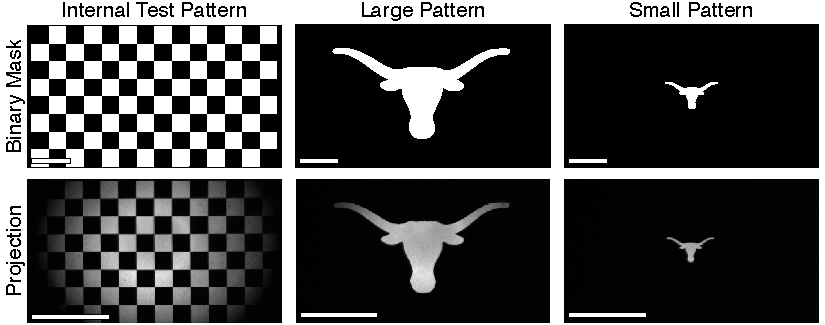
\includegraphics{figures/chapter_2/dmdalignment.pdf}
    \caption{
        \label{fig:dmdalignment}
        Test patterns used to perform and verify alignment of the DMD-projected light (Scale bars = 1 mm).
    }
\end{figure}

Alignment of the DMD was performed using a second camera placed at the focus of the objective lens to directly image the projected light. This was necessary because the two dichroic beamsplitters prevent excitation light from reaching the primary system camera. An internal checkerboard pattern on the DLP LightCrafter and external binary masks were used to verify that the diffraction orders were properly converging onto the sample plane (Figure \ref{fig:dmdalignment}C). These images also verified the 0.5x optical magnification applied to the projected patterns. Because the DMD has a rectangular aspect ratio, the circular illuminating beam slightly underfills the active area, resulting in some peripheral mirrors being unusable for patterning. The Gaussian beam also produces a non-uniform intensity profile, which would be problematic for intensity-based imaging techniques but fortunately has minimal effect on lifetime measurements.

In order to use the Speckle Software to define arbitrarily-shaped patterns, the camera FOV must be registered with the projection area of the DMD. An affine transform is used to translate, scale, shear, and rotate the mask from the camera coordinate system to the DMD coordinate system without linear distortion. The matrix representation of the 2D affine transform using homogeneous coordinates is defined as:
%
% Equation - Affine Transform
\begin{equation}
    \label{eq:affine}
    \begin{bmatrix}
        x' \\
        y' \\
        1  \\
    \end{bmatrix}
    =
    \begin{bmatrix}
        a & b & c \\
        d & e & f \\
        0 & 0 & 1 \\
    \end{bmatrix}
    \begin{bmatrix}
        x \\
        y \\
        1 \\
    \end{bmatrix}
\end{equation}
%
where $(x,y)$ represent camera coordinates and $(x',y')$ represent DMD coordinates. The Speckle Software performs the registration by prompting the user to identify the positions of three sequentially projected points in the camera FOV and then solving Equation \ref{eq:affine} for the six coefficients of the transformation matrix. The user can then define an ROI using the speckle contrast image for reference and the affine transform will be applied to the mask as it is uploaded to the DMD (Figure \ref{fig:dmdregistration}).

% Figure - DMD Registration
\begin{figure}
    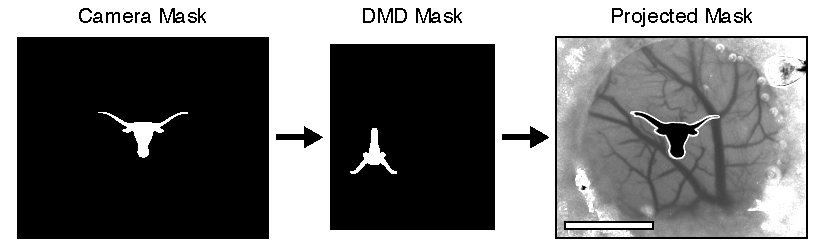
\includegraphics{figures/chapter_2/dmdregistration.pdf}
    \caption{
        \label{fig:dmdregistration}
        Example of the affine image transformation applied to the camera coordinate space binary mask and the resulting DMD-projected pattern as imaged using LSCI (Scale bar = 1 mm).
    }
\end{figure}

%%%%%%%%%%%%%%%%%%%%%%%%%%%%%%%%%%%%%%%%%%%%%%%%%%%%%%%%%%%%%%%%%%%%%%%%%%%%%%%
\subsection{Laser Diode Stability}

Laser diode stability is extremely important when performing LSCI because the technique is sensitive to changes in coherence and lasing wavelength. Regulated thermoelectric cooling (TEC) has been shown to significantly improve the stability of laser diode operation and reduce noise during LSCI measurements \cite{Richards:2016hy}. Identifying stable laser operating conditions requires adjusting the laser diode current and the TEC temperature setpoint. The 685 nm laser diode used for LSCI has a recommended operating current of 75 mA and exhibits temperature-dependent changes in slope efficiency and lasing wavelength.

The diode was tested under different operating conditions by imaging a static piece of paper and examining the stability of the intensity and speckle contrast over time within the center quadrant of the camera FOV (Figure \ref{fig:laserstability}A). A total of nine conditions were tested with laser diode currents varied between 65, 70, and 75 mA and TEC temperatures varied between 17, 18, and 19 $^\circ$C. The system was allowed to stabilize for five minutes after changing a parameter before acquiring LSCI data for ten minutes.

% Figure - Laser Diode Stability
\begin{figure}
    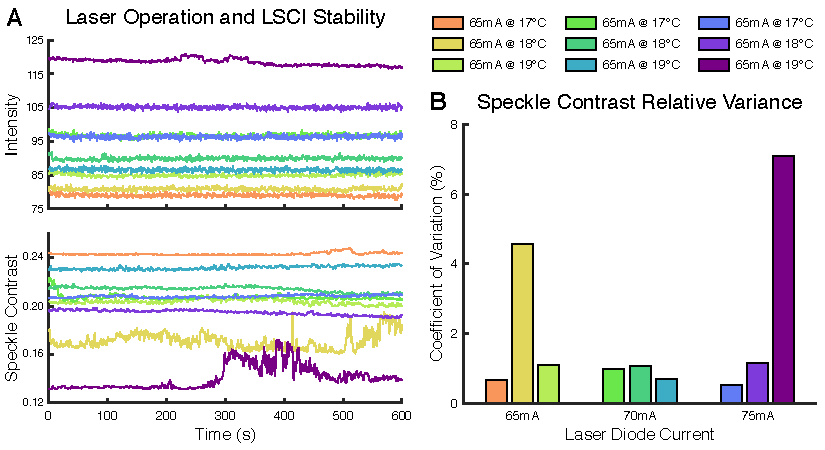
\includegraphics{figures/chapter_2/laserstability.pdf}
    \caption{
        \label{fig:laserstability}
        \textbf{(A)} Intensity and speckle contrast timecourses under different laser diode operating conditions. \textbf{(B)} Measurement of relative variance between the different speckle contrast data to identify the optimal laser diode operating conditions.
    }
\end{figure}

As expected, higher laser diode operating currents resulted in higher intensity values. With the exception of the 75 mA current at 19 $^\circ$C condition, minimal fluctuations in intensity were seen over time. However, the speckle contrast measurements exhibited much greater variation within and between acquisitions. Significant mode hopping, where the laser suddenly switches to a different resonator mode resulting in a discrete jump in the center wavelength, can be seen in both the 65 mA current at 18 $^\circ$C and 75 mA current at 19 $^\circ$C conditions. Mode hopping manifests in diode lasers because of temperature transients and non-ideal TEC operating temperatures. These fluctuations severely impact LSCI measurements and operating conditions must be optimized to mitigate them.

In order to identify the best operating parameters, the coefficient of variation (CV = $\sigma$ / $\mu$) for each speckle contrast timecourse was computed (Figure \ref{fig:laserstability}B). This statistic allows for the comparison of variation between data series with different means, with smaller values indicating less variance. Based on this metric, the 75 mA laser diode current at the 17 $^\circ$C TEC setpoint offered the best stability (CV = 0.05\%) for LSCI measurements. These settings were used exclusively throughout the remainder of this dissertation.



%%%%%%%%%%%%%%%%%%%%%%%%%%%%%%%%%%%%%%%%%%%%%%%%%%%%%%%%%%%%%%%%%%%%%%%%%%%%%%%
% Section 2.2 - Oxygen Tension Measurements in Cuvettes
%%%%%%%%%%%%%%%%%%%%%%%%%%%%%%%%%%%%%%%%%%%%%%%%%%%%%%%%%%%%%%%%%%%%%%%%%%%%%%%
\section{Oxygen Tension Measurements in Cuvettes}

Phosphorescence lifetime measurements were first tested in normoxic and anoxic cuvettes of 10 $\mu$M Oxyphor PtG4. The normoxic cuvette was prepared under ambient conditions and therefore has \ce{pO2} equivalent to that of air ($\sim$150 mmHg). The anoxic (0 mmHg) cuvette was created using the enzymatic reaction between glucose and glucose oxidase to scavenge oxygen from the sealed environment \cite{Lo:1997he}. Phosphorescent decays ($n$ = 200) were acquired using both 445 and 637 nm excitation with all DMD pixels in the ON position. The resulting decay curves were averaged and fitted for $\tau$ and the calibration curve used to lookup the corresponding \ce{pO2} value (Figure \ref{fig:cuvette}A). For both excitation wavelengths, the normoxic cuvette \ce{pO2} was 152 mmHg while the anoxic cuvette \ce{pO2} was 0 mmHg (Figure \ref{fig:cuvette}B).

% Figure - Cuvette pO2 Measurements
\begin{figure}
    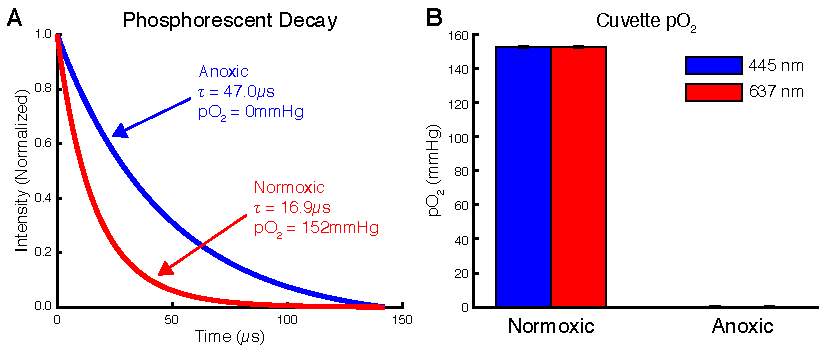
\includegraphics{figures/chapter_2/cuvette.pdf}
    \caption{
        \label{fig:cuvette}
        \textbf{(A)} Averaged phosphorescent decay curves ($n$ = 200) in anoxic and normoxic cuvette environments with fitted lifetimes and their corresponding \ce{pO2} values. \textbf{(B)} Excitation wavelength does not affect measured \ce{pO2}.
    }
\end{figure}

%%%%%%%%%%%%%%%%%%%%%%%%%%%%%%%%%%%%%%%%%%%%%%%%%%%%%%%%%%%%%%%%%%%%%%%%%%%%%%%
\subsection{Fitted Lifetime Discrepancy}

The lifetimes of fluorescent and phosphorescent decays are independent of excitation wavelength. Targeting the Soret or Q band absorption maxima of a porphyrin should result in identical measurements of $\tau$ since internal conversion and vibrational relaxation occur on picosecond timescales. However, discrepancies in the phosphorescent decays were identified between 445 and 637 nm excitation (Figure \ref{fig:offsetcorrection}A). Fitting the exponential decays produced different values of $\tau$ from the same cuvette depending on the excitation. Since $\tau$ cannot vary with wavelength, this discrepancy likely arises because the two lasers are modulated using different mechanisms. The 445 nm laser is optically modulated using an AOM while the 637 nm laser is electronically modulated using its driver. Ideally both light sources should be modulated using the same technique to eliminate differences in bandwidth and modulation depth that can manifest in the optical signal.

In order to correct for this error, the exponential decay fitting process was modified with a temporal offset to ensure that both wavelengths would produce the same lifetime values. Figure \ref{fig:offsetcorrection}B depicts the relationship between the offset and the resulting fits for $\tau$ in the normoxic cuvette. As the offset is increased, the fitting is biased towards longer lifetimes. The optimal offsets were identified at $t$ = 21.50 $\mu$s for 445 nm excitation and $t$ = 26.54 $\mu$s for 637 nm excitation. These offsets result in a fitted $\tau$ = 16.993 $\mu$s (\ce{pO2} = 152 mmHg) and are used throughout this dissertation. A major disadvantage of this strategy is the waste of phosphorescent signal. In the normoxic cuvette, these offsets correspond to 96\% and 60\% of the peak phosphorescence intensity for 445 and 637 nm excitation, respectively. While the exact percentage scales with $\tau$, this can have detrimental effects on fitting performance for weak signals.

% Figure - Offset Correction
\begin{figure}
    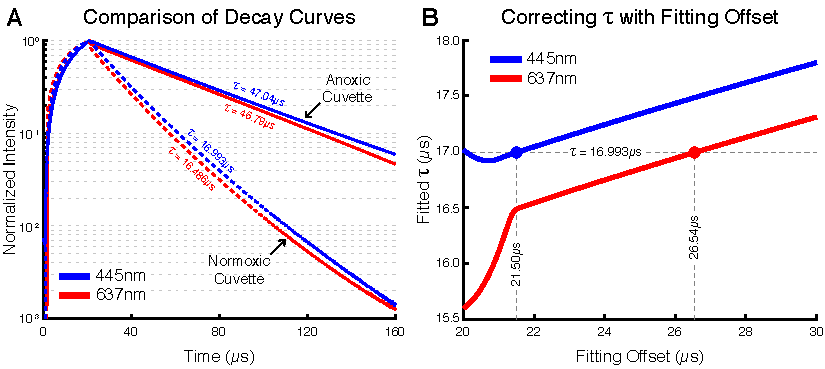
\includegraphics{figures/chapter_2/offsetcorrection.pdf}
    \caption{
        \label{fig:offsetcorrection}
        \textbf{(A)} 445 and 637 nm excitation produce different phosphorescent decay curves in identical samples. \textbf{(B)} Introducing an offset into the exponential decay fitting process corrects the wavelength-dependent lifetime discrepancy.
    }
\end{figure}

%%%%%%%%%%%%%%%%%%%%%%%%%%%%%%%%%%%%%%%%%%%%%%%%%%%%%%%%%%%%%%%%%%%%%%%%%%%%%%%
\subsection{Limitations of the Calibration Curve} \label{ssec:calibration_limit}

Performing measurements on the normoxic cuvette revealed a limitation of the Oxyphor PtG4 calibration curve (Figure \ref{fig:oxyphor_ptg4}B), which has a maximum \ce{pO2} of 160 mmHg. While this is well beyond normal physiological values, any measurements conducted in animal subjects receiving supplemental oxygen would require using the Stern-Volmer relationship to convert $\tau$ into \ce{pO2}. However, the calibration curve does not fit the Stern-Volmer relationship particularly well ($R^2$ = 0.9729) and results in a discontinuous transition between the two methods (Figure \ref{fig:sternvolmerfit}). Lifetime measurements shorter than 16.6 $\mu$s will abruptly drop from 160 to 134 mmHg. Because of this deviation from the expected kinetics, there is significant uncertainty in the true \ce{pO2} values beyond the range of the empirical data. Despite this limitation, the combination of the calibration curve and the fitted Stern-Volmer parameters are used throughout this dissertation. The calibration curve is used when 16.6 $\mu$s $\ge \tau$ $\ge$ 47 $\mu$s and the Stern-Volmer relationship is used when $\tau$ \textless{} 16.6 $\mu$s. When $\tau$ \textgreater{} 47 $\mu$s ($\tau_0$), \ce{pO2} is set to 0 mmHg.

% Figure - Stern-Volmer Fit
\begin{figure}
    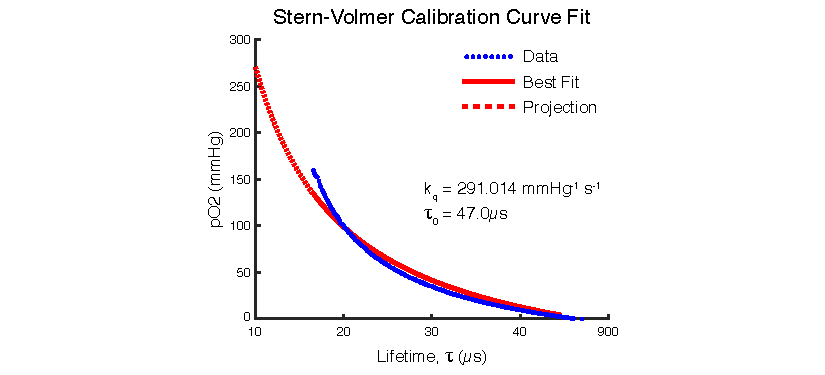
\includegraphics{figures/chapter_2/sternvolmerfit.pdf}
    \caption{
        \label{fig:sternvolmerfit}
        Least-squares fitting of the Stern-Volmer relationship to the Oxyphor PtG4 calibration data and the resulting prediction for lifetimes down to 10 $\mu$s. For $\tau > \tau_0$, \ce{pO2} is set to 0 mmHg.
    }
\end{figure}



%%%%%%%%%%%%%%%%%%%%%%%%%%%%%%%%%%%%%%%%%%%%%%%%%%%%%%%%%%%%%%%%%%%%%%%%%%%%%%%
% Section 2.3 - Demonstration of Acute In Vivo Imaging
%%%%%%%%%%%%%%%%%%%%%%%%%%%%%%%%%%%%%%%%%%%%%%%%%%%%%%%%%%%%%%%%%%%%%%%%%%%%%%%
\section{Demonstration of Acute \textit{In Vivo} Imaging}

The system was tested \textit{in vivo} using mice (CD-1, male, 25-30 g, Charles River) with permanent cranial window implants (see Appendix \ref{app:cranial_window}) that afford optical access to the surface of the brain. The window was positioned over the frontoparietal cortex approximately 2 mm rostral from bregma and 0.5 mm lateral from the sagittal suture. Animals with clear and healthy cranial windows were selected for use after at least two weeks of recovery post-surgery. The subject was anesthetized with medical air vaporized isoflurane (1.5\%) via nose-cone inhalation and placed supine in a head-fixed stereotaxic frame (Narishige Scientific Instrument Lab). Oxygen gas was intentionally avoided to prevent hyperoxia from interfering with the \ce{pO2} measurements. Vitals including oxygen saturation, heart rate, and breath rate were monitored via pulse oximetry (MouseOx, Starr Life Sciences) and temperature was regulated with a feedback heating pad (DC Temperature Controller, FHC). Oxyphor PtG4 was administered via retro-orbital injection into the venous sinus for a target blood plasma concentration of 5 $\mu$M. The subject was then placed under the dual-modality system for imaging.

% Figure - Static Speckle and ICT
\begin{figure}
    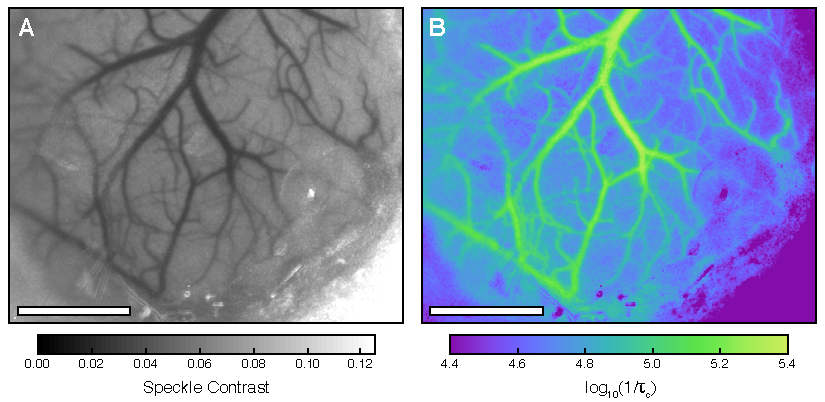
\includegraphics{figures/chapter_2/staticspeckle.pdf}
    \caption{
        \label{fig:staticspeckle}
        \textbf{(A)} Speckle contrast and \textbf{(B)} ICT images of the mouse cortex (Scale bars = 1mm).
    }
\end{figure}

Figure \ref{fig:staticspeckle} depicts an averaged ($n$ = 45) speckle contrast image and its corresponding ICT image highlighting the vasculature of the cortex. Speckle contrast images in this document are displayed using a grayscale colormap spanning the full range of the speckle contrast histogram. ICT images are displayed on a logarithmic scale using a perceptually-balanced colormap \cite{Niccoli:vx} spanning the full range of the ICT histogram. Compared to the speckle contrast image, the ICT image more clearly depicts the flow profiles within the larger vessels.

Static oxygen tension measurements were acquired from two arterioles, two veins, and one parenchyma region using both the 445 and 637 nm excitation lasers (Figure \ref{fig:staticpO2}A). Patterns were displayed at 1 Hz for a total of 5 seconds with 2500 phosphorescent decays averaged per ROI. The measured \ce{pO2} within each region aligns well with physiological expectations with both arterioles exhibiting higher \ce{pO2} than the venous or parenchyma areas (Figure \ref{fig:staticpO2}B). The effects of wavelength can be seen as 445 nm excitation resulted in a broader range of \ce{pO2} values (48-83 mmHg) compared to 637 nm excitation (75-82 mmHg). Despite differences in absolute value, the trend of arterioles having greater \ce{pO2} than parenchyma, which in turn has greater \ce{pO2} than veins, exists for both excitation wavelengths. Since lifetime does not depend upon excitation wavelength (Figure \ref{fig:cuvette}B), these differences likely arise because of increased penetration depth at the longer wavelength.

% Figure - Static pO2
\begin{figure}
    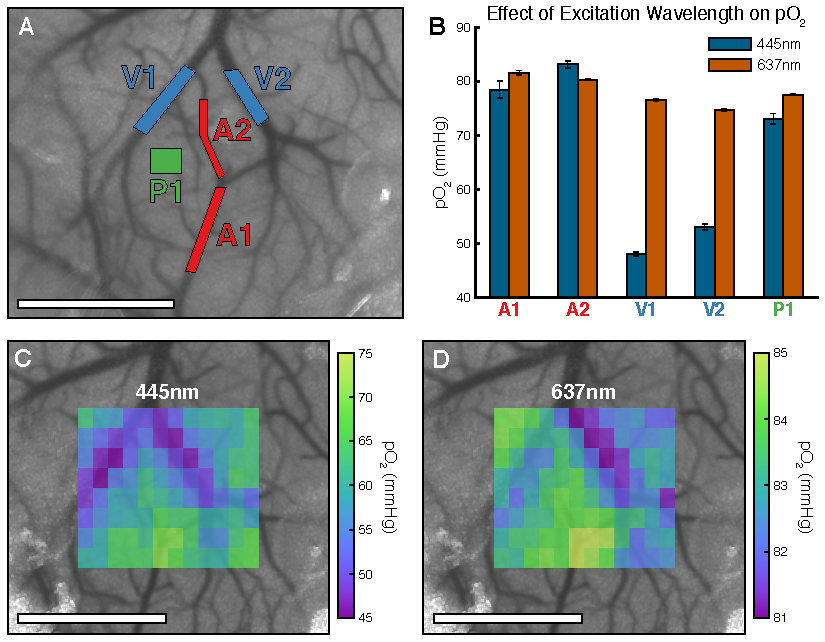
\includegraphics{figures/chapter_2/staticpO2.pdf}
    \caption{
        \label{fig:staticpO2}
        \textbf{(A)} Speckle contrast image of cortical flow overlaid with regions targeted for \ce{pO2} measurements. Two descending arterioles (A1, A2), two veins (V1, V2), and one parenchyma region (P1) were examined. The projected patterns ranged between 0.014 - 0.046 mm$^2$ in area. \textbf{(B)} \ce{pO2} measurements within the targeted regions conducted using both 445 and 637 nm excitation of Oxyphor PtG4 (mean $\pm$ s.d.). \textbf{(C)} 445 nm and (d) 637 nm \ce{pO2} maps produced using tiled excitation patterns covering a 1.2 x 1.0 mm area. Each individual tile has a projected area of 0.012 mm$^2$ (Scale bars = 1mm).
    }
\end{figure}

In order to obtain a more comprehensive look at vascular oxygenation within the camera FOV, an array of 12 x 8 rectangular tiles was sequentially projected using the DMD. The tiles were displayed at 10 Hz with 250 decays averaged per pattern for a total acquisition time of 9.6 seconds. The resulting \ce{pO2} maps (Figure \ref{fig:staticpO2}C-D) coarsely follow the visible surface vasculature. As expected, the large branching vein has lower \ce{pO2} values compared to the arteriole approaching from the bottom of the FOV or the surrounding parenchyma. 445 nm excitation again resulted in a wider range of \ce{pO2} values (45-85 mmHg) compared to 637 nm excitation (81-85 mmHg).

%%%%%%%%%%%%%%%%%%%%%%%%%%%%%%%%%%%%%%%%%%%%%%%%%%%%%%%%%%%%%%%%%%%%%%%%%%%%%%%
\subsection{Hyperoxic Challenge}

The ability to detect changes in cortical oxygen tension was tested using an hyperoxic challenge. The oxygen fraction of inspired air under anesthesia was increased from 21\% (normoxia) to 100\% and then decreased back to normoxia for recovery. Hyperoxia was maintained for five minutes and \ce{pO2} measurements using 445 nm excitation were acquired at the end of each stage from three regions covering an arteriole, venule, and parenchyma (Figure \ref{fig:hyperoxicchallenge}A). The patterns were displayed at 1 Hz with 2500 phosphorescent decays averaged per ROI. A large increase in \ce{pO2} was detected during the hyperoxic state across all three regions (Figure \ref{fig:hyperoxicchallenge}B) with the arteriole experiencing the largest net increase (+120 mmHg). The \ce{pO2} remained slightly elevated above baseline values several minutes later during the post-hyperoxia recovery stage.

The measured lifetime in the arteriole during hyperoxia was only 13.1 $\mu$s and therefore exceeds the limits of the Oxyphor PtG4 calibration curve (Section \ref{ssec:calibration_limit}). The Stern-Volmer relationship was used to calculate the \ce{pO2} and likely underestimates the actual value. While it is counterintuitive for the arteriole to experience the largest increase in \ce{pO2}, similar results were seen during hyperoxic retinal imaging in both mice and rats \cite{Shonat:2003ia}.

% Figure - Hyperoxic Challenge
\begin{figure}
    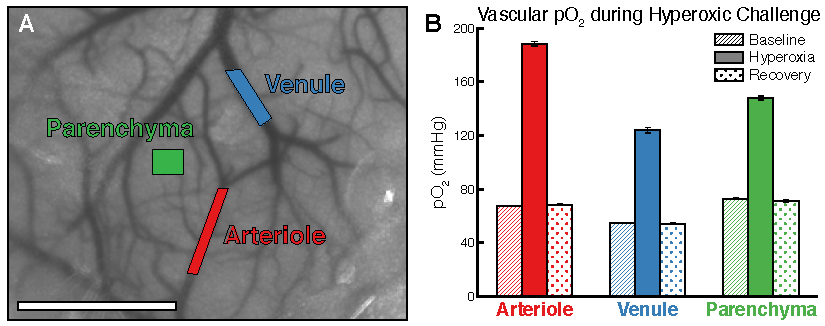
\includegraphics{figures/chapter_2/hyperoxicchallenge.pdf}
    \caption{
        \label{fig:hyperoxicchallenge}
        \textbf{(A)} Speckle contrast image depicting three regions (arteriole, venule, and parenchyma) targeted for 445 nm \ce{pO2} measurements during an hyperoxic challenge. \textbf{(B)} Static \ce{pO2} during baseline, hyperoxic, and recovery stages for each of the targeted vessels (mean $\pm$ s.d.). (Scale bar = 1mm).
    }
\end{figure}

%%%%%%%%%%%%%%%%%%%%%%%%%%%%%%%%%%%%%%%%%%%%%%%%%%%%%%%%%%%%%%%%%%%%%%%%%%%%%%%
\subsection{Effects of Excitation Wavelength on Measured \ce{pO2}}

The results in Figure \ref{fig:staticpO2} revealed major differences in measured \ce{pO2} depending on excitation wavelength. The static \ce{pO2} measurements under 445 nm illumination spanned a range five times larger than that of 637 nm illumination. This discrepancy was most noticeable in venous regions, with the shorter excitation wavelength resulting in \ce{pO2} values around 50 mmHg whereas the longer wavelength resulted in values around 75 mmHg. Since depth penetration is heavily dependent upon wavelength \cite{Deng:2003kb}, the difference is likely the result of photons sampling a much larger volume of tissue during 637 nm illumination.

An estimate of transmission through a surface vessel at both wavelengths can be obtained using the Beer-Lambert Law. Because scattering increases the distance traveled by photons in tissue, this represents the most conservative estimate of the effect of wavelength on transmission. Assuming hemoglobin is the primary absorber in blood plasma with a concentration of 2.3 mM\cite{Robles:2010cw} and 95\% SaO2, the transmittance at 445 nm and 637 nm through a 100 μm arteriole is 0.9\% and 96.5\%, respectively. As excitation wavelength approaches the tissue optical window, the transmission of incident light significantly increases. The 445 nm light is almost entirely confined within a vessel of that caliber and does not extensively sample deeper microvasculature. Because the 637 nm light penetrates further into the brain, the measured pO2 is skewed away from the vascular value and is more representative of a bulk volumetric average. This is consistent with prior Monte Carlo modeling that found fluorescence primarily originates from within large surface vasculature at shorter wavelengths \cite{Davis:2011wj}. As excitation wavelength increases, a larger fraction of the detected fluorescence originates from beyond the vessel.

These results indicate that excitation wavelength must be considered when performing single-photon fluorescent or phosphorescent measurements using dyes with multiple excitation maxima. Longer wavelengths would not be ideal for studying surface vasculature because of the increased penetration depth but would be better suited for examining parenchyma regions or bulk areas. Conversely, the limited penetration depth of shorter excitation wavelengths, especially in vasculature, make them ideal for restricting measurements to only surface tissue.



%%%%%%%%%%%%%%%%%%%%%%%%%%%%%%%%%%%%%%%%%%%%%%%%%%%%%%%%%%%%%%%%%%%%%%%%%%%%%%%
% Section 2.4 - Discussion
%%%%%%%%%%%%%%%%%%%%%%%%%%%%%%%%%%%%%%%%%%%%%%%%%%%%%%%%%%%%%%%%%%%%%%%%%%%%%%%
\section{Discussion}

The dual-modality imaging system combining LSCI and oxygen-dependent quenching of phosphorescence is a purely optical, non-contact platform for measuring CBF and \ce{pO2}. The system builds upon prior work by Ponticorvo and Dunn \cite{Ponticorvo:2010uv} by using structured illumination to overcome the traditional limitations of lifetime imaging. Spatially patterning excitation light with a DMD allows for the use of a point detector, which offers both high sensitivity and speed for the collection of the phosphorescent signal. Ultimately, the spatial and temporal resolutions of the phosphorescent measurements are limited by noise. Regions as small as 0.01 mm$^2$ could reliably be excited at a pattern repetition rate of 10 Hz with 250 phosphorescent decay curves accumulated per ROI. Because intensity of the excitation light scales with the number of DMD pixels in the ON state, larger patterns could allow for even faster pattern rates at the expense of averaging (e.g. 100 Hz with 25 decays averaged per ROI). However, a 10 Hz pattern rate is more than sufficient for visualizing many dynamic physiological events in the brain.



%%%%%%%%%%%%%%%%%%%%%%%%%%%%%%%%%%%%%%%%%%%%%%%%%%%%%%%%%%%%%%%%%%%%%%%%%%%%%%%
% END Chapter 2
%%%%%%%%%%%%%%%%%%%%%%%%%%%%%%%%%%%%%%%%%%%%%%%%%%%%%%%%%%%%%%%%%%%%%%%%%%%%%%%


% Chapter 3 - Spatially-Targeted Photothrombotic Stroke
%%%%%%%%%%%%%%%%%%%%%%%%%%%%%%%%%%%%%%%%%%%%%%%%%%%%%%%%%%%%%%%%%%%%%%%%%%%%%%%
% Chapter 3 - Spatially-Targeted Photothrombotic Stroke
%%%%%%%%%%%%%%%%%%%%%%%%%%%%%%%%%%%%%%%%%%%%%%%%%%%%%%%%%%%%%%%%%%%%%%%%%%%%%%%

\chapter{Spatially-Targeted Photothrombotic Stroke} \label{ch:photothrombosis}

Animal models of ischemic stroke are extensively used to study the mechanisms of neuronal death and recovery and to perform preliminary testing on neuroprotective interventions. While there are numerous techniques for inducing focal ischemia, the majority rely upon occlusion of the middle cerebral artery (MCA) and its branches. The MCA is the largest cerebral artery in the brain and the most common vessel involved with human ischemic events \cite{Sicard:2009ku}. The models that can most reliably reproduce the lesions and pathophysiology of human stroke (e.g. ischemic core and penumbra) offer the best experimental platforms for preclinical research.

Intraluminal MCA occlusion (MCAo) is the most widely used technique and is performed by introducing a monofilament suture into the internal carotid artery to block blood flow to the MCA \cite{Kozuimi:1986bd}. This model is capable of inducing both permanent and transient focal ischemia similar to that of human stroke and does not require craniotomy. The procedure results in large-scale infarct volumes (21-45\% of ipsilateral hemisphere) that most closely resemble malignant infarction in humans \cite{Carmichael:2005gk}. However, the majority of human strokes are much smaller in size (4.5-14\%) \cite{Carmichael:2005gk, Brott:1989bl}, making traditional MCAo a poor model for studying recovery at a similar scale. Distal MCAo produces smaller infarcts limited to the cerebral hemisphere but requires performing a craniotomy to physically access the target vessel \cite{Doyle:2014bz}. Embolic MCAo relies upon the introduction of microspheres or the induction of thrombotic clots to occlude downstream vasculature. Particle size dictates the extent and localization of the infarction, which are more variable than traditional or distal MCAo \cite{Carmichael:2005gk}. Vasoconstrictors such as Endothelin-1 (ET-1) can be injected intracerebrally in the proximity of the MCA to induce transient ischemia with a dose-dependent recovery of blood flow \cite{Sicard:2009ku}. Surgical electrocauterization or direct clipping of the MCA can also be performed to induce permanent or reversible ischemia but require craniotomy.

The photothrombosis model uses intravascular photooxidation to generate well-defined cortical lesions \cite{Watson:1985bp}. Photosensitive dyes such as rose bengal are injected intravenously and irradiated with light to produce singlet oxygen, which causes localized endothelial damage initiating platelet aggregation and thrombus formation \cite{Dietrich:1987wh}. Rose bengal has been extensively utilized as a photothrombotic agent \cite{Grome:1988bx, Parthasarathy:2010vo} and has well-characterized pharmacokinetics with fast clearance from the body \cite{Klaassen:1976kg}. A significant advantage of the photothrombotic model is the ability to stereotactically control the position and size of the infarct to target specific functional regions. However, the technique results in rapid vasogenic edema, which is thought to restrict the development of the ischemic penumbra and local reperfusion \cite{Carmichael:2005gk}.

The DMD in the imaging system offers a new method for targeting photothrombosis that allows for increased control over the stroke induction process compared to conventional techniques that only illuminate a single focal volume. Entire vessels, arbitrarily-shaped regions, or even multiple locations can be simultaneously occluded by using the DMD to pattern the irradiating light. By specifically targeting vessels, collateral photooxidative damage to the surrounding tissue can be minimized. This chapter details modifications made to the imaging system to perform DMD-targeted photothrombosis and an \textit{in vivo} demonstration of the technique in mice. The targeted photothrombosis technique was described in a methods paper published in \textit{Neurophotonics} \cite{Sullender:2018ff}.



%%%%%%%%%%%%%%%%%%%%%%%%%%%%%%%%%%%%%%%%%%%%%%%%%%%%%%%%%%%%%%%%%%%%%%%%%%%%%%%
% Section 3.1 - Instrumentation Modifications
%%%%%%%%%%%%%%%%%%%%%%%%%%%%%%%%%%%%%%%%%%%%%%%%%%%%%%%%%%%%%%%%%%%%%%%%%%%%%%%
\section{Instrumentation Modifications}

The system was modified (Figure \ref{fig:systemschematic_2}) to perform photothrombotic stroke with the addition of a 532 nm laser (200 mW, AixiZ LLC). The packaged diode laser has a 2 mm collimated output that operates at a fixed current with convection cooling. A neutral density filter (OD 1.0, NE10A-A, Thorlabs, Inc.) was used to attenuate the laser intensity by an order of magnitude down to 20 mW. A longpass dichroic beamsplitter (490 nm cutoff, DMLP490, Thorlabs, Inc.) was used to coalign the 532 nm laser with the other two lasers for coupling into the fiber optic patch cord. The green light can then be patterned by the DMD for targeted photothrombosis. \ce{pO2} measurements can be acquired simultaneously during photothrombosis induction because of the system's spectral separation, but are limited to only the stroke target region.

% Figure - System Schematic (Ver. 2)
\begin{figure}
    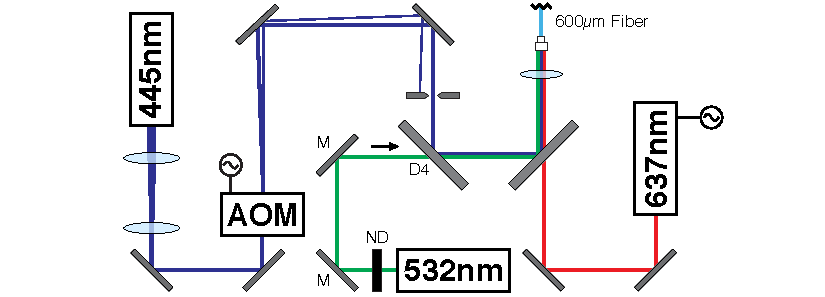
\includegraphics{figures/chapter_3/systemschematic_2.pdf}
    \caption{
        \label{fig:systemschematic_2}
        The optical system was modified with the addition of a 532 nm laser coupled into the fiber optic patch cord for DMD-targeted photothrombosis.
    }
\end{figure}



%%%%%%%%%%%%%%%%%%%%%%%%%%%%%%%%%%%%%%%%%%%%%%%%%%%%%%%%%%%%%%%%%%%%%%%%%%%%%%%
% Section 3.2 - Targeted Photothrombosis Induction
%%%%%%%%%%%%%%%%%%%%%%%%%%%%%%%%%%%%%%%%%%%%%%%%%%%%%%%%%%%%%%%%%%%%%%%%%%%%%%%
\section{Targeted Photothrombosis Induction} \label{sec:photothrombosis_induction}

Targeted photothrombosis was demonstrated \textit{in vivo} using anesthetized (1.5\% isoflurane in medical air) mice with permanent cranial window implants. Rose bengal was administered intravenously via retro-orbital injection (50 $\mu$L, 15 mg/mL) and the subject was immediately exposed to DMD-patterned green light for 5-10 minutes. Descending arterioles were the primary targets because they serve as bottlenecks in the cortical oxygen supply \cite{Nishimura:2007hk}. Target vessels were identified based on vascular orientation and \textit{a posteriori} knowledge. Because Oxyphor PtG4 has minimal absorbance of green light, \ce{pO2} measurements can be simultaneously acquired while performing photothrombosis. However, the measurements were limited to only the region being targeted for occlusion. LSCI was used to monitor clot formation within the targeted area and to control the progression of the occlusion. The open source image registration software \texttt{elastix} \cite{Klein:2010gr} was used during post-processing to correct the speckle contrast images for any motion relative to the beginning of the acquisition. This would infrequently occur if the animal was not properly secured in the stereotaxic frame. The automatic intensity-based transform allowing for rotation and translation was applied to each speckle contrast frame. The computed speckle contrast inverse correlation times (ICT = $1/\tau_c$) were then baselined against pre-stroke values to provide an estimate of the relative change in blood flow (rICT = $\tau_{c,initial}/\tau_c$).

Figure \ref{fig:photothrombosisacute} depicts the targeted photothrombotic occlusion of a descending arteriole that is likely a distal branch of the MCA. The red overlay in Figure \ref{fig:photothrombosisacute}A highlights the 0.09 mm$^2$ region irradiated with spatially-patterned green light for 420 seconds. \ce{pO2} measurements were continuously acquired from the same region at 1 Hz with 2500 decays averaged per record. The series of speckle contrast images depict the progression of the photothrombotic occlusion as the targeted vessel rapidly underwent stenosis and flow was significantly reduced. After only two minutes of exposure, the targeted vessel was indistinguishable from the surrounding parenchyma.

% Figure - Acute Photothrombosis
\begin{figure}
    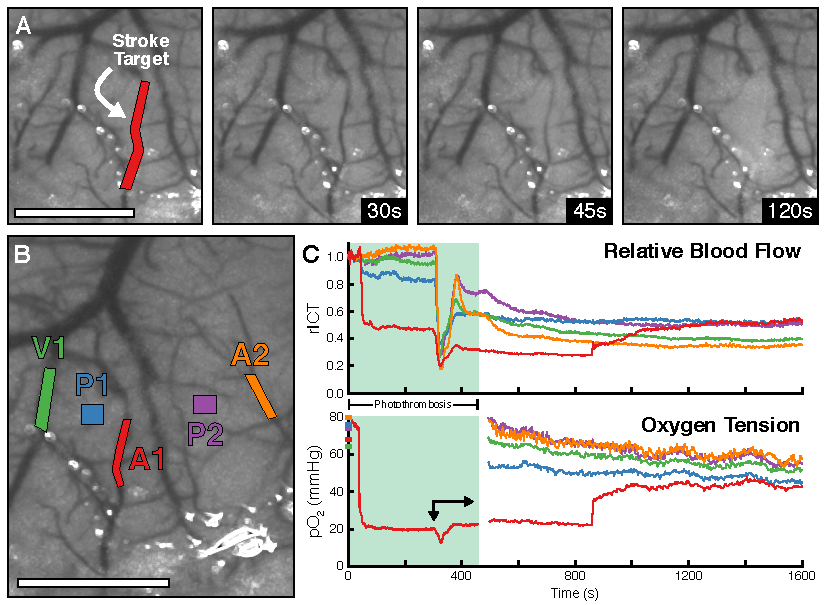
\includegraphics{figures/chapter_3/photothrombosisacute.pdf}
    \caption[\textbf{(A)} Speckle contrast images depicting the occlusion of a descending arteriole using DMD-targeted photothrombosis. The red overlay indicates the 0.09 mm$^2$ region simultaneously illuminated for occlusion and \ce{pO2} measurements. \textbf{(B)} Two arterioles (A1, A2), one vein (V1), and two parenchyma regions (P1, P2) were targeted for \ce{pO2} measurements after stroke induction. \textbf{(C)} Relative blood flow and \ce{pO2} within the targeted regions during and after photothrombosis. The green-shaded section indicates irradiation of the targeted arteriole. The arrow indicates the propagation of an ischemia-induced depolarization event (Scale bars = 1 mm).]{
        \label{fig:photothrombosisacute}
        \textbf{(A)} Speckle contrast images depicting the occlusion of a descending arteriole using DMD-targeted photothrombosis. The red overlay indicates the 0.09 mm$^2$ region simultaneously illuminated for occlusion and \ce{pO2} measurements. \textbf{(B)} Two arterioles (A1, A2), one vein (V1), and two parenchyma regions (P1, P2) were targeted for \ce{pO2} measurements after stroke induction. \textbf{(C)} Relative blood flow and \ce{pO2} within the targeted regions during and after photothrombosis. The green-shaded section indicates irradiation of the targeted arteriole. The arrow indicates the propagation of an ischemia-induced depolarization event (Scale bars = 1 mm). Adapted from \cite{Sullender:2018ff}.
    }
\end{figure}

% Figure - PID Propagation
\begin{figure}
    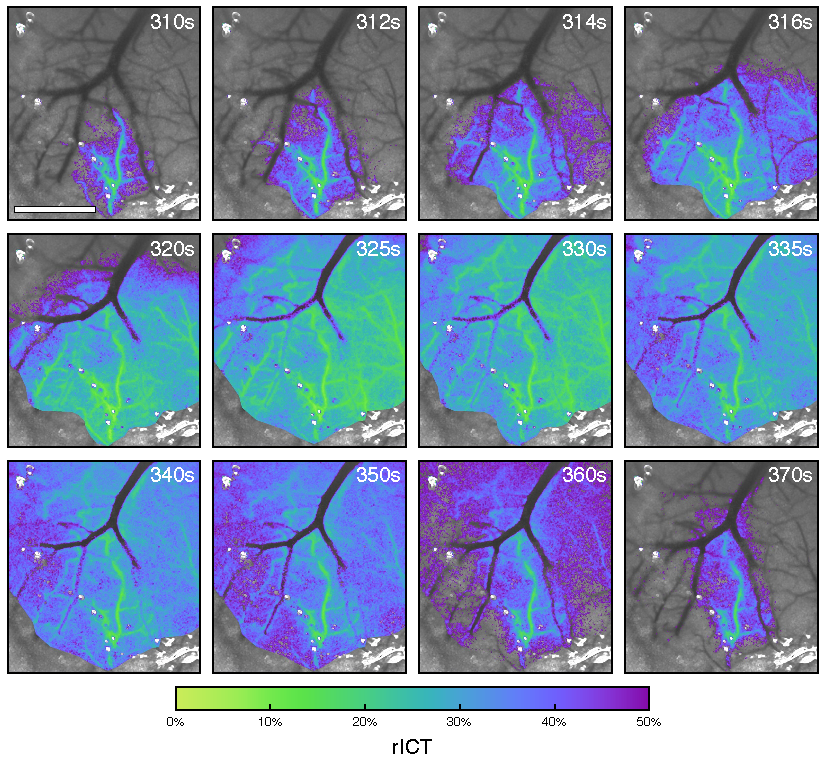
\includegraphics{figures/chapter_3/pidsequence.pdf}
    \caption{
        \label{fig:pidsequence}
        Relative flow during an ischemia-induced depolarization event that results in the expansion of the flow deficit. The depolarization has minimal effect upon the large draining vein. (Scale bar = 1 mm).
    }
\end{figure}

Figure \ref{fig:photothrombosisacute}B depicts the five regions (two arterioles, one vein, two parenchyma) targeted for dynamic relative blood flow and \ce{pO2} measurements. The first arteriole region (A1) is the same vessel targeted for photothrombotic occlusion. The resulting timecourses of relative blood flow and \ce{pO2} within each region can be seen in Figure \ref{fig:photothrombosisacute}C. By $t$ = 120 seconds, flow within the targeted arteriole had decreased to \textless50\% of baseline and \ce{pO2} had dropped from 80 mmHg to only 20 mmHg. Over the following several minutes, flow also decreased in the nearby parenchyma and venous regions (P1 and V1) and increased slightly in the distal second arteriole region (A2). The propagation of an ischemia-induced depolarization event \cite{Shin:2006dc, Dreier:2011gz} can be seen beginning at $t$ = 300 seconds, with sharp reductions in both relative blood flow and \ce{pO2}. As the depolarization subsided, flow within the targeted arteriole further decreased to \textless35\% of baseline flow while the \ce{pO2} returned to pre-depolarization levels around 20 mmHg. Flow in all other regions remained depressed immediately following the depolarization. Figure \ref{fig:pidsequence} overlays relative ICT on speckle contrast imagery to depict the spatial extent of the depolarization and the resulting increase in deficit area. This global reduction in flow following a spreading depolarization is consistent with previous studies using other stroke models \cite{Shin:2006dc, Nakamura:2010wp}.

Photothrombosis irradiation was stopped at $t$ = 420 seconds and \ce{pO2} measurements from all five ROIs were initiated. Patterns were displayed at 2 Hz with 1250 decays averaged per record. Flow and \ce{pO2} decreased over the remaining 20 minutes of the imaging session across all regions except for A1. At $t$ = 860 seconds, the targeted vessel partially reperfused, causing an abrupt increase in both relative blood flow (+6 percentage points) and \ce{pO2} (+15 mmHg). By the end of the imaging session, flow had increased within A1 to 55\% of baseline and \ce{pO2} to 42 mmHg, likely indicating further reperfusion of the vessel.



%%%%%%%%%%%%%%%%%%%%%%%%%%%%%%%%%%%%%%%%%%%%%%%%%%%%%%%%%%%%%%%%%%%%%%%%%%%%%%%
% Section 3.3 - Chronic Post-Stroke Hemodynamics
%%%%%%%%%%%%%%%%%%%%%%%%%%%%%%%%%%%%%%%%%%%%%%%%%%%%%%%%%%%%%%%%%%%%%%%%%%%%%%%
\section{Chronic Post-Stroke Hemodynamics} \label{sec:chronic_hemodynamics}

The chronic progression of the ischemic lesion was monitored for eight days following photothrombosis. The subject was anesthetized (1.5\% isoflurane in medical air) and positioned on the stereotaxic frame such that the speckle contrast imagery was aligned with previous acquisitions. Imaging sessions were kept as short as possible (\textless30 minutes) to avoid over-exposure to isoflurane. The perfusion of the occluded arteriole and broader effects on cortical flow were tracked using LSCI as shown in Figure \ref{fig:photothrombosischronic}A. Tiled \ce{pO2} maps acquired using both 445 and 637 nm excitation (Figure \ref{fig:photothrombosischronic}B-C) reveal the spatial extent of the oxygen deficit. The broad value range of the colormap masks the smaller \ce{pO2} differences between arterioles and venules. A large gradient can be seen between the occluded vessel and surrounding tissue on Days +1 and +2 despite partial reperfusion of the targeted vessel. This gradient resembles the ischemic penumbra that the photothrombotic technique rarely produces \cite{Carmichael:2005gk}. By Day +5, the targeted arteriole had fully reperfused and the hypoxic region recovered to near baseline.

% Figure - Chronic Photothrombosis
\begin{figure}
    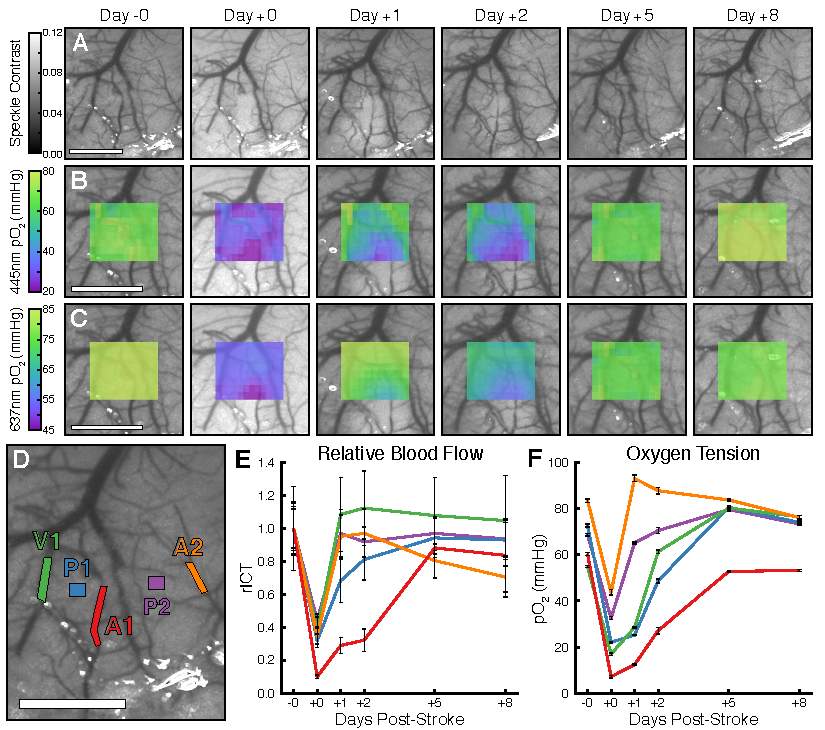
\includegraphics{figures/chapter_3/photothrombosischronic.pdf}
    \caption[Progression of the ischemic lesion over eight days as imaged with \textbf{(A)} LSCI, \textbf{(B)} 445 nm tiled \ce{pO2}, and \textbf{(C)} 637 nm tiled \ce{pO2} measurements. Day -0 measurements were taken immediately prior to photothrombosis induction and Day +0 measurements were taken immediately after. \textbf{(D)} Two arterioles (A1, A2), one vein (V1), and two parenchyma regions (P1, P2) were targeted for chronic \textbf{(E)} relative blood flow and \textbf{(F)} 445 nm \ce{pO2} measurements (mean $\pm$ s.d.). The relative blood flow was baselined against Day -0 measurements. (Scale bars = 1 mm).]{
        \label{fig:photothrombosischronic}
        Progression of the ischemic lesion over eight days as imaged with \textbf{(A)} LSCI, \textbf{(B)} 445 nm tiled \ce{pO2}, and \textbf{(C)} 637 nm tiled \ce{pO2} measurements. Day -0 measurements were taken immediately prior to photothrombosis induction and Day +0 measurements were taken immediately after. \textbf{(D)} Two arterioles (A1, A2), one vein (V1), and two parenchyma regions (P1, P2) were targeted for chronic \textbf{(E)} relative blood flow and \textbf{(F)} 445 nm \ce{pO2} measurements (mean $\pm$ s.d.). The relative blood flow was baselined against Day -0 measurements. (Scale bars = 1 mm). Adapted from \cite{Sullender:2018ff}.
    }
\end{figure}

The same five regions (two arterioles, one vein, and two parenchyma) used during the acute photothrombosis measurements were also targeted for chronic relative blood flow and \ce{pO2} measurements (Figure \ref{fig:photothrombosischronic}D-F). The relative blood flow was calculated using the spatial average of the pre-stroke (Day -0) ICT measurements as the baseline. The first post-stroke measurements (Day +0) were taken immediately after the induction of photothrombosis and revealed global deficits in both blood flow and \ce{pO2}. This systemic change is likely the result of the spreading depolarization, which have previously been shown to cause global reductions in CBF using other stroke models \cite{Shin:2006dc, Nakamura:2010wp}. The blood flow and \ce{pO2} within the ROIs mirror the recovery seen in the spatially-resolved results with the vessel fully reperfusing by Day +5.

The speed of this recovery is faster than previous traditional photothrombotic inductions performed by the lab, which took 3-4 weeks to return to baseline flow levels \cite{Schrandt:2015gu}. This discrepancy can be explained by the smaller area targeted for photothrombosis (0.09 mm$^2$ vs. 0.28 mm$^2$) and the lower irradiance (\textless15 mW/mm$^2$ vs. 72 mW/mm$^2$) within the area of illumination, which resulted in a less severe ischemic lesion. Confinement of the excitation light to only within the targeted arteriole minimized collateral damage to the surrounding vasculature and parenchyma and allowed the infarct to manifest downstream of the occlusion. The lack of reperfusion is also a common critique of the traditional photothrombotic model of stroke \cite{Carmichael:2005gk}.

%%%%%%%%%%%%%%%%%%%%%%%%%%%%%%%%%%%%%%%%%%%%%%%%%%%%%%%%%%%%%%%%%%%%%%%%%%%%%%%
\subsection{Persistence of Oxyphor PtG4 \textit{In Vivo}}

Oxyphor PtG4 is a large molecule with a molecular weight around 35 kDa. The majority of its size arises from the PEGylated hydrophobic dendrimer surrounding the PtTBP core used to increase biocompatibility and lifetime stability. Pilot experiments with Oxyphor PdG4, an analog with a palladium core, found that it was retained in the bloodstream for hours and readily accumulated within tumors via the enhanced permeability and retention effect \cite{Esipova:2011hi}. This allowed animals to be imaged up to a day after being injected with 10 $\mu$M Oxyphor PdG4.

Oxyphor PtG4 persists in the bloodstream significantly longer than previously reported in literature. Strong phosphorescent decay curves have be obtained up to two weeks after an initial injection of the dye with a target blood plasma concentration of 5 $\mu$M. The mouse utilized for the targeted photothrombosis and eight days of chronic hemodynamic imaging described above was only administered a single dose of Oxyphor PtG4 on the first day of imaging. While this allows for efficient usage of a limited supply of dye, it remains unclear how and where the probe persists in the bloodstream for such an extended period of time. Phosphorescent intensity does decrease day-to-day, which means that the probe does not remain indefinitely. However, if the protective dendrimer structure is being degraded, then the reliability of the lifetime measurements is a major concern. Unfortunately, it would be difficult to validate the correct \ce{pO2} using a different technique \textit{in vivo} or to replicate the appropriate testing conditions \textit{in vitro}. In order to mitigate the impact of these uncertainties, supplemental injections of Oxyphor PtG4 for a blood plasma concentration of 5 $\mu$M are administered weekly in subjects being used for chronic imaging.



%%%%%%%%%%%%%%%%%%%%%%%%%%%%%%%%%%%%%%%%%%%%%%%%%%%%%%%%%%%%%%%%%%%%%%%%%%%%%%%
% Section 3.4 - Functional Effects of Targeted Photothrombosis
%%%%%%%%%%%%%%%%%%%%%%%%%%%%%%%%%%%%%%%%%%%%%%%%%%%%%%%%%%%%%%%%%%%%%%%%%%%%%%%
\section{Functional Effects of Targeted Photothrombosis}

A comprehensive comparison between traditional and artery-targeted photothrombosis using the DMD was performed by Taylor A. Clark\footnote{The results of this section are adapted from a manuscript currently under review as `T Clark, C Sullender, S Kazmi, B Speetles, M Williamson, D Palmberg, A Dunn, and T Jones. Artery targeted photothrombosis enlarges the vascular penumbra, instigates peri-infarct neovascularization and models upper extremity impairments.' CS developed the instrumentation and performed the targeted photothrombosis inductions. TC performed the experiments, analyzed the results, and wrote the manuscript.}. This section presents results on the functional impairments caused by targeted photothrombosis in the motor cortex. A total of 23 young-adult (4-6 months) C57/Bl6/YFP-H mice were used to examine the impact on skilled forelimb function, with subjects undergoing targeted photothrombosis ($n$ = 13) or sham procedures ($n$ = 10). Mice with cranial windows were anesthetized with \ce{O2}-vaporized isoflurane (4\% induction, 1.5-2\% maintenance) via nose-cone inhalation and placed in a head-fixed stereotaxic frame. Vitals including oxygen saturation, heart rate, and breath rate were monitored via pulse oximetry and temperature was regulated with a feedback heating pad. Rose bengal was administered via retro-orbital injection (50 $\mu$L, 15 mg/mL) and photothrombosis was initiated after a 30 second delay. Sham subjects received injections of sterile saline. DMD-targeted photothrombosis was performed by irradiating pial arteries supplying the forelimb region of the motor cortex as defined from intracortical mappings \cite{Tennant:2011cx} for 10 minutes. In order to account for variations in the size and caliber of the vessels, a range of 1-3 branches were illuminated with an average total targeted area of 0.15 $\pm$ 0.021 mm$^2$. The primary vessels targeted in all subjects were distal branches of the MCA. Photothrombosis progression was monitored in real-time using LSCI.

%%%%%%%%%%%%%%%%%%%%%%%%%%%%%%%%%%%%%%%%%%%%%%%%%%%%%%%%%%%%%%%%%%%%%%%%%%%%%%%
\subsection{Single Seed Retrieval Task}

The resulting impact on forelimb function was examined by testing performance during a skilled reaching task. The task was a variation of the single seed retrieval task \cite{Chen:2014hy} where mice are trained to reach for and obtain a millet seed placed on a platform outside of transparent training chamber. A pair of 4 mm wide vertical openings on the left and right sides of the chamber permitted the mice to reach through with only the corresponding paw (Figure \ref{fig:reachingtask}A). The external platform contained three wells at varying distances from each opening for the placement of seeds (Figure \ref{fig:reachingtask}B). Two of the wells were centered on the opening and positioned at distances 3 mm (Position 1) and 7 mm (Position 2) away from the chamber. The third well (Position 3) was placed 2 mm lateral of the distal edge of the opening and 5 mm away from the chamber.

The preferred limb for reaching was determined during shaping by allowing the mice to reach for millet seeds with either limb when seeds were placed immediately outside both openings. The preferred-for-reaching limb was defined as the first one used to make five consecutive reach attempts (Figure \ref{fig:reachingtask}C). For the remaining 2-3 days of the shaping phase, mice were encouraged to reach for a single seed placed in Position 1 with their preferred-for-reaching limb. The shaping phase concluded once mice were able to successfully retrieve the seed 10 times (Figure \ref{fig:reachingtask}D). The mice then underwent 10 consecutive days of training sessions, each comprised of 30 trials. Seeds were placed in one of the three positions per trial, with each position recurring ten times per training session in a randomized order. Mice were permitted four reaching attempts per trial with a successful reaching attempt defined as grasping the seed and bringing it inside the chamber to its mouth. Unsuccessful reaching attempts included missing, displacing, or dropping the seed prior to eating.

% Figure - Reaching Task
\begin{figure}
    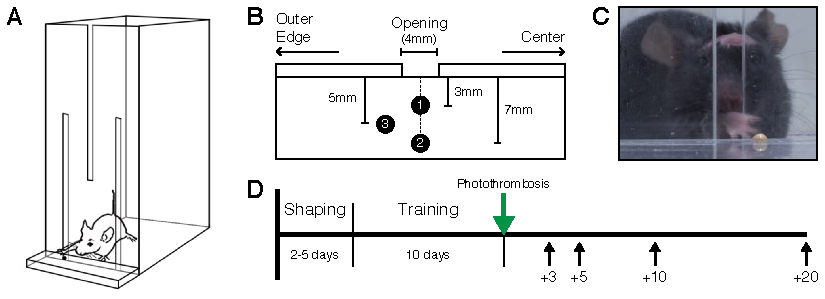
\includegraphics{figures/chapter_3/reachingtask.pdf}
    \caption[\textbf{(A)} The transparent training chamber and pair of 4 mm vertical openings used for performing the reaching task. \textbf{(B)} The three positions used for seed placement outside of each opening. \textbf{(C)} A mouse reaching for a seed. \textbf{(D)} Training and measurement timeline for the behavioral experiments.]{
        \label{fig:reachingtask}
        \textbf{(A)} The transparent training chamber and pair of 4 mm vertical openings used for performing the reaching task. Adapted from \cite{Chen:2014hy}. \textbf{(B)} The three positions used for seed placement outside of each opening. \textbf{(C)} A mouse reaching for a seed. \textbf{(D)} Training and measurement timeline for the behavioral experiments.
    }
\end{figure}

The mean asymptotic performance (average of the last two training days) prior to photothrombosis inductions for each of the three positions was 0.44 $\pm$ 0.02 (Position 1), 0.3 $\pm$ 0.02 (Position 2), and 0.2 $\pm$ 0.01 (Position 3). Because performance on Position 3 was much lower compared to the other two positions, it was excluded from analysis. Results were reported as the percent of successful reaches per reaching attempt for Positions 1 and 2. Performance was tested on Days 3, 5, 10, and 20 following photothrombosis induction or sham procedure. The SPSS Statistics (IBM Corp.) software package was used to examine reaching performance between the stroke and sham groups over time using two-way repeated measures ANOVA.

%%%%%%%%%%%%%%%%%%%%%%%%%%%%%%%%%%%%%%%%%%%%%%%%%%%%%%%%%%%%%%%%%%%%%%%%%%%%%%%
\subsection{Tissue Processing and Analysis of Lesion Volume}

Animals were euthanized 30 days after photothrombosis with sodium pentobarbital and transcardially perfused with 0.1 M phosphate buffered saline and 4\% paraformaldehyde. The brains were extracted and stored in 4\% paraformaldehyde for no more than 48 hours before using a vibrating blade microtome (VT1000S, Leica Biosystems) to slice 40 $\mu$m coronal sections spaced 240 $\mu$m apart between approximately 1.34 mm anterior to 0.58 mm posterior to bregma. The sections were Nissl stained in order to identify viable cortical tissue and imaged with 17x magnification. The cortical volume was estimated with Cavalieri's Principle \cite{Rosen:1990bf} using Neurolucida (MBF Bioscience) by computing the product of the summed section areas and the distance between sections. Lesion volume was then calculated as the difference between cortical volumes of the contralateral and ipsilateral hemispheres \cite{Tennant:2011cx}.

%%%%%%%%%%%%%%%%%%%%%%%%%%%%%%%%%%%%%%%%%%%%%%%%%%%%%%%%%%%%%%%%%%%%%%%%%%%%%%%
\subsection{Results}

Artery-targeted photothrombosis in the motor cortex significantly impaired performance on the skilled reaching task compared to the sham control on Days 3, 5, and 10 (Figure \ref{fig:functionalimpairment}A). Two-way repeated measures ANOVA of reaching performance over time revealed a significant effect in the stroke vs. sham grouping ($F_{[1,23]}$ = 145.50, $p$ \textless{} 0.0001) but no significant interaction in grouping over time ($F_{[3,69]}$ = 2.77, $p$ = 0.06). By Day 20, performance on the reaching test in the stroke group was similar to that of the sham group. This transience is likely a byproduct of the relatively small infarcts (Figure \ref{fig:functionalimpairment}B-C). Nevertheless, these results suggest that artery-targeted photothrombosis is suitable for creating reproducible focal lesions in the motor cortex that can be used to model upper extremity impairments.

% Figure - Functional Impairment
\begin{figure}
    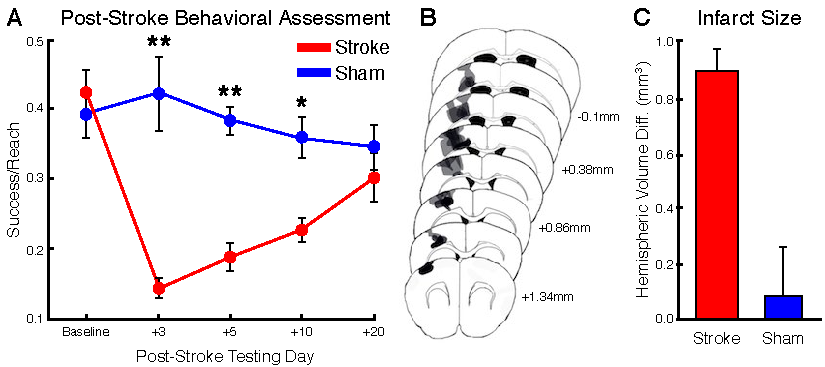
\includegraphics{figures/chapter_3/functionalimpairment.pdf}
    \caption{
        \label{fig:functionalimpairment}
        \textbf{(A)} Baseline and post-stroke reaching performance measured by the ratio of successfully retrieved seeds per reaching attempt (mean $\pm$ s.e.). Artery-targeted photothrombosis impaired performance on post-stroke Days 3, 5, and 10 (\textbf{**} $p$ \textless{} 0.001, \textbf{*} $p$ \textless{} 0.02) compared to the sham procedure. \textbf{(B)} Averaged lesion reconstructions overlaid on coronal templates. The numbers indicate the anterior-to-posterior coordinates relative to bregma. \textbf{(C)} Volume difference between the contralateral and ipsilateral hemispheres as an estimate of infarct size (mean $\pm$ s.e.).
    }
\end{figure}



%%%%%%%%%%%%%%%%%%%%%%%%%%%%%%%%%%%%%%%%%%%%%%%%%%%%%%%%%%%%%%%%%%%%%%%%%%%%%%%
% Section 3.5 - Discussion
%%%%%%%%%%%%%%%%%%%%%%%%%%%%%%%%%%%%%%%%%%%%%%%%%%%%%%%%%%%%%%%%%%%%%%%%%%%%%%%
\section{Discussion}

The addition of a green laser to the DMD illumination pathway facilitates the induction of arbitrarily-shaped photothrombotic lesions. The system allows for greater control over the spatial characteristics of the induced stroke (e.g. size and location) and permits targeting multiple vessels simultaneously. The creation of an extended occlusion within a single arteriole using targeted photothrombosis was demonstrated for the first time. This is a significant change from existing photothrombotic techniques that generally rely upon broad illumination to occlude a large volume of vasculature \cite{Watson:1985bp, Schrandt:2015gu} or highly-focused light to occlude a single microvessel \cite{Schaffer:2006fb}. The previous iteration of this system could only induce occlusions within a large region relative to the FOV and \ce{pO2} measurements could not be simultaneously acquired \cite{Ponticorvo:2010uv}.

While tissue \ce{pO2} during ischemic depolarizations have been previously examined \cite{vonBornstadt:2015dj}, the results reported in \textit{Neurophotonics} \cite{Sullender:2018ff} represent the first quantification of the acute vascular \ce{pO2} response to a depolarization event and the first chronic hemodynamic tracking of an ischemic infarct. The depolarization resulted in a global flow reduction across all regions, which is consistent with previous reports using other stroke models \cite{Shin:2006dc,Nakamura:2010wp}. Within the targeted arteriole, the blood flow reduction is of greater magnitude (-58\%) than the corresponding decrease in \ce{pO2} (-44\%), which eventually recovers to slightly above pre-depolarization levels. Unfortunately, it is difficult to predict how the \ce{pO2} responded to the depolarization across the other regions, but it likely mirrored the LSCI results. The chronic measurements revealed a rapid recovery over the course of five days with the spatial extent of the ischemic lesion clearly visible on the first two days post-stroke. Functional tests revealed that the artery-targeted photothrombotic model of ischemic stroke could be used to produce detectable and reproducible impairments in upper extremity motor skills. The deficits recovered over the course of several weeks and only produced minor lesions.



%%%%%%%%%%%%%%%%%%%%%%%%%%%%%%%%%%%%%%%%%%%%%%%%%%%%%%%%%%%%%%%%%%%%%%%%%%%%%%%
% END Chapter 3
%%%%%%%%%%%%%%%%%%%%%%%%%%%%%%%%%%%%%%%%%%%%%%%%%%%%%%%%%%%%%%%%%%%%%%%%%%%%%%%


% Chapter 4 - Improving Cerebral Blood Flow Measurements with Multi-Exposure Speckle Imaging
%%%%%%%%%%%%%%%%%%%%%%%%%%%%%%%%%%%%%%%%%%%%%%%%%%%%%%%%%%%%%%%%%%%%%%%%%%%%%%%
% Chapter 4 - Improving Cerebral Blood Flow Measurements with Multi-Exposure Speckle Imaging
%%%%%%%%%%%%%%%%%%%%%%%%%%%%%%%%%%%%%%%%%%%%%%%%%%%%%%%%%%%%%%%%%%%%%%%%%%%%%%%

\chapter{Improving Cerebral Blood Flow Measurements with Multi-Exposure Speckle Imaging} \label{ch:mesi}

While the conventional LSCI technique can provide reliable measurements of relative flow, it is incapable of quantifying absolute baseline values. This complicates the chronic study and inter-animal comparisons of blood flow dynamics because variations in imaging conditions cannot be properly accounted for by the underlying model. This has not prevented LSCI from being used to study chronic changes in flow (see Section \ref{sec:chronic_hemodynamics}), but has limited the observations to predominantly qualitative interpretations \cite{Armitage:2010ga}. The technique has also been shown to underestimate large changes in flow and fails to produce reliable measurements in the presence of static scatters \cite{Parthasarathy:2008el}.

Multi-exposure speckle imaging (MESI) is an extension to traditional LSCI theory that accounts for static scattering and produces a more robust estimate of $\tau_c$ using multiple camera exposure times \cite{Parthasarathy:2008el}. These improvements are achieved by accounting for the heterodyne mixing of dynamic and static scattering contributions, the non-ergodicity of light, and exposure-independent noise. The model described by Parthasarathy \textit{et al.} \cite{Parthasarathy:2008el} again relates the measured $K$ with $\tau_c$:

% Equation - MESI Equation
\begin{equation}
    \label{eq:mesi}
    \resizebox{\textwidth}{!}{$
    K(T,\tau_c) =
        \left(
        \beta\rho^2\frac{e^{-2x} - 1 + 2x}{2x^2} +
        4\beta\rho(1 - \rho)\frac{e^{-x} - 1 + x}{x^2} +
        \beta(1 - \rho)^2 +
        \nu_{ne} +
        \nu_{noise}
        \right)^{1/2}
    $}
\end{equation}

\noindent where $x = T/\tau_c$, $T$ is the camera exposure time, $\beta$ is the same normalization factor that accounts for speckle averaging effects, $\rho$ is the fraction of light that is dynamically scattered, $\nu_{ne}$ is the constant variance due to nonergodic light, and $\nu_{noise}$ is the exposure-independent instrument noise. For simplicity, $\nu_{ne}$ and $\nu_{noise}$ are typically merged into a single noise parameter ($\nu_{noise}$). Similar to Equation \ref{eq:bandyopadhyay}, this expression assumes that detected photons only experience single scattering interactions and that the underlying particle motion has a Lorentzian velocity distribution. A scaling term representing the number of average dynamic scattering events can be included with $x$ to account for multiple scattering interactions \cite{Kazmi:2015du}. In the absence of static scatterers, $\rho \to 1$ and Equation \ref{eq:mesi} simplifies to Equation \ref{eq:bandyopadhyay}, excluding the noise terms. In the presence of only static scatterers, then $\rho \to 0$ and $K$ reduces to a constant $\beta(1 - \rho)^2 + \nu_{noise}$ and is independent of exposure time. This represents the upper limit of the speckle variance ($K^2$) as $T$ approaches infinity. The lower limit as $T$ approaches 0 is $\beta + \nu_{noise}$, which can be approximated with just $\beta$ because the noise will only constitute a small percentage of the total value.

A minimum of four speckle contrast images acquired at different exposure times are necessary to fit Equation \ref{eq:mesi} for the four unknown variables ($\beta$, $\rho$, $\tau_c$, $\nu_{noise}$). In practice, 15 images spanning three decades of exposure times (50 $\mu$s - 80 ms) are typically utilized to sample as much of the underlying flow distribution as possible. The MESI model has improved the quantitative accuracy of flow measurements in controlled microfluidic environments \cite{Parthasarathy:2008el, Kazmi:2015du} and closely approximates the results of direct autocorrelation measurements \cite{Kazmi:2015ji}. The technique has enabled the chronic study of CBF across multiple animals and improved the robustness of flow deficit measurements during stroke \cite{Parthasarathy:2010vo, Kazmi:2013hp, Schrandt:2015gu}. This chapter details an upgrade to the imaging system to perform MESI and further validation of its capabilities.



%%%%%%%%%%%%%%%%%%%%%%%%%%%%%%%%%%%%%%%%%%%%%%%%%%%%%%%%%%%%%%%%%%%%%%%%%%%%%%%
% Section 4.1 - Instrumentation Modifications
%%%%%%%%%%%%%%%%%%%%%%%%%%%%%%%%%%%%%%%%%%%%%%%%%%%%%%%%%%%%%%%%%%%%%%%%%%%%%%%
\section{Instrumentation Modifications}

The instrumentation necessary for performing MESI is similar to traditional LSCI but requires precise control over both the camera exposure time and the laser intensity. Varying the exposure time alone would result in shot noise overwhelming the speckle signal at longer exposure times because of differences in intensity. However, by modulating the amplitude of the illuminating laser light, the average intensity of the images, and therefore the shot noise, can be held constant. Passive optical devices such as AOMs have historically been used to avoid the bandwidth and dynamic range limitations of direct laser diode modulation.

Figure \ref{fig:systemschematic_3} depicts the modifications made to the LSCI illumination pathway in order to perform MESI with the system. The same 685 nm laser diode (50 mW, HL6750MG, Thorlabs, Inc.) was collimated using an aspheric lens (C240TME-B, Thorlabs, Inc.) and the beam diameter was reduced to 1 mm. The light was modulated using a 100 MHz AOM (3100-125 AOM + 1110AF-AIFO-1.0 RF Driver, Gooch \& Housego) with the first order diffraction isolated and relayed to obliquely illuminate the sample. The camera was also upgraded (acA1920-155um, 1920 x 1200 pixels, Basler AG) because the previous model did not support trigger-based control of exposure duration, which is important for implementing MESI. The new camera also offered more convenient USB 3.0 connectivity, higher maximum frame rate (164 fps), lower dark noise, and increased dynamic range. While the pixel resolution was almost doubled, only a subset of the overall sensor array was used (1200 x 1000 pixels), resulting in a FOV of 3.6 x 3.0 mm.

% Figure - System Schematic (Ver. 3)
\begin{figure}
    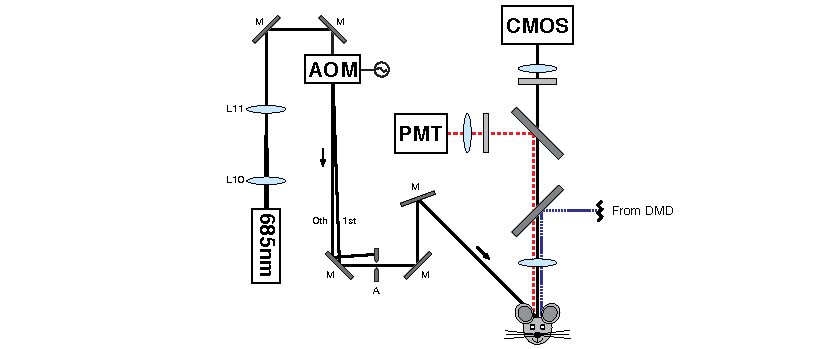
\includegraphics{figures/chapter_4/systemschematic_3.pdf}
    \caption{
        \label{fig:systemschematic_3}
        The optical system was modified to perform MESI with the addition of an AOM to modulate the 685 nm laser used for LSCI.
    }
\end{figure}

%%%%%%%%%%%%%%%%%%%%%%%%%%%%%%%%%%%%%%%%%%%%%%%%%%%%%%%%%%%%%%%%%%%%%%%%%%%%%%%
\subsection{Acquisition Control}

The MESI acquisition process is controlled by a combination of the Speckle Software and a standalone MATLAB (MathWorks, Inc.) script. The software was updated to allow the camera to perform "Trigger Width Exposure Mode" acquisitions, where the duration of a hardware trigger signal directly controls the exposure time of each frame. The MATLAB script used the ANSI C NI-DAQmx library (National Instruments Corp.) to operate a multifunction I/O device (USB-6363, National Instruments Corp.) to produce the camera exposure trigger signals and AOM modulation voltages (Figure \ref{fig:mesitimingschematic}). Both waveforms were generated at 1 MHz with identical pulse durations but a slight temporal offset (+25 $\mu$s delay for the AOM signal) to guarantee that the actual camera exposures and the laser pulses were synchronized in time. This was validated using the “Exposure Active” output signal from the camera and a photodiode (PDA36A, Thorlabs, Inc.) directly measuring the modulated laser.

A complete MESI frame consists of 15 raw intensity images (8-bit) each acquired with a different exposure time for an effective frame rate of 2.5 fps without any averaging. This is significantly slower than standard LSCI and insufficient to properly sample faster hemodynamic processes. Because of limitations with the Speckle Software, the speckle contrast images cannot be computed for real-time visualization during an acquisition. This requires the speckle contrast images to be generated during post-processing. A standard MESI acquisition produces data at a rate of 178 MB/s.

% Figure - MESI Timing
\begin{figure}
    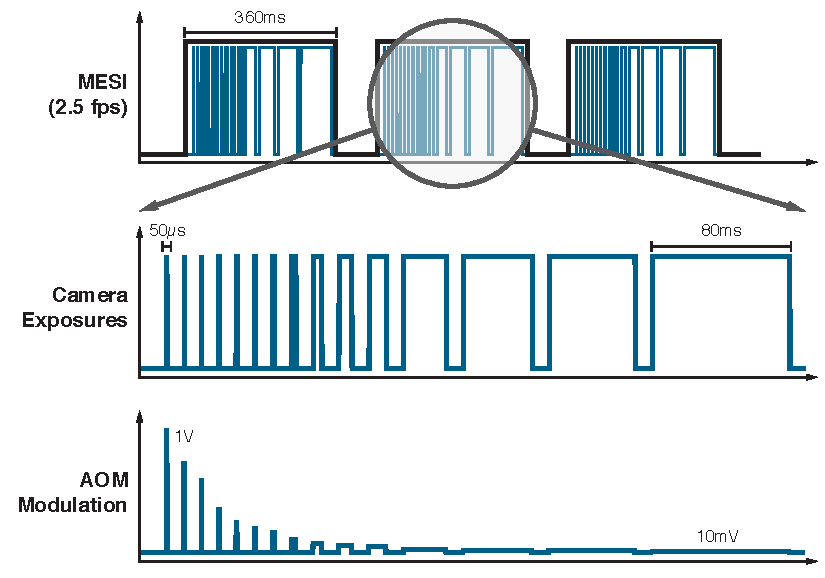
\includegraphics{figures/chapter_4/mesitimingschematic.pdf}
    \caption{
        \label{fig:mesitimingschematic}
        Timing paradigm for MESI camera exposure triggers and AOM modulation voltages. The integration of each AOM pulse over time is equal.
    }
\end{figure}

%%%%%%%%%%%%%%%%%%%%%%%%%%%%%%%%%%%%%%%%%%%%%%%%%%%%%%%%%%%%%%%%%%%%%%%%%%%%%%%
\subsection{Calibration Procedure}

The AOM modulation voltages for each exposure are determined using the calibration procedure outlined in Figure \ref{fig:mesicalibration}. This process ensures that shot noise is held constant across all exposures by equalizing the total amount of light used to produce each image. Because the reflectivity of the imaging surface varies by sample, the calibration must be performed prior to each MESI experiment.

% Figure - MESI Calibration
\begin{figure}
    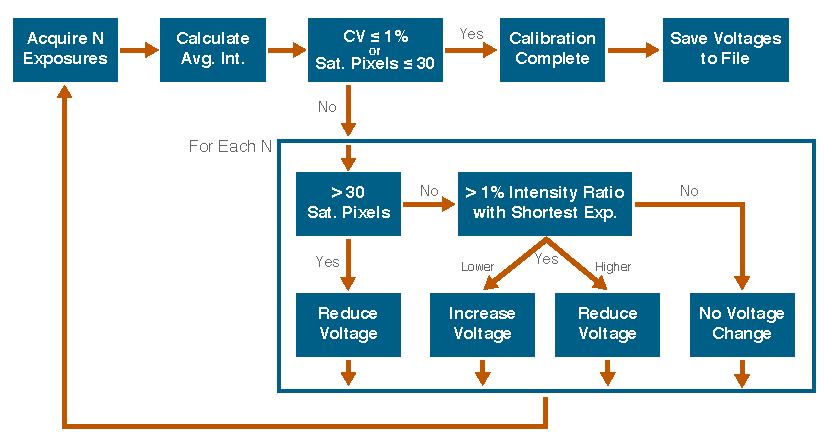
\includegraphics{figures/chapter_4/mesicalibration.pdf}
    \caption{
        \label{fig:mesicalibration}
        Overview of the MESI calibration process that attempts to equalize the raw image intensities while minimizing saturated pixels across all $N$ exposures.
    }
\end{figure}

The initial guess for the modulation voltages is generated using a power law function confined between 0-1 V. These voltages are used to acquire a complete MESI frame containing 15 raw intensity images from different exposures. The average intensity and total number of saturated pixels within a user-defined region is then calculated for each image. If the overall coefficient of variation and the number of saturated pixels are less than the defined thresholds, then the intensities are equalized and the calibration is complete. However, if the average intensity variation is too high or if there are too many saturated pixels, then each of the modulation voltages are adjusted accordingly using the shortest exposure time as the target intensity. This process repeats recursively until the stop conditions are achieved. A typical calibration will take between 30-50 iterations and complete within less than a minute.

% Figure - MESI Raw
\begin{figure}
    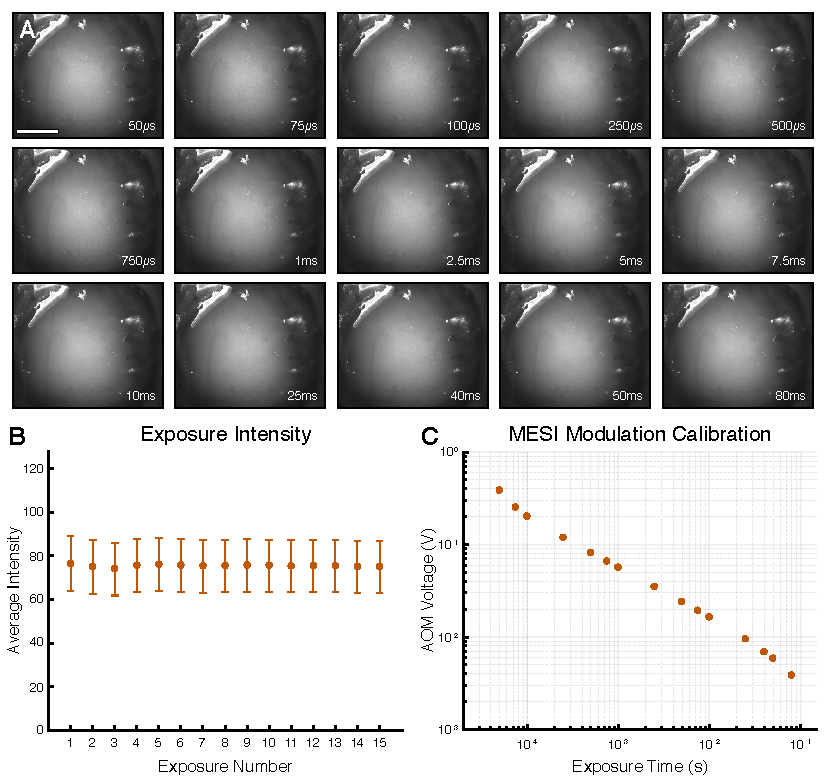
\includegraphics{figures/chapter_4/rawmesi.pdf}
    \caption{
        \label{fig:rawmesi}
        \textbf{(A)} Raw images of a cranial window from each of the 15 MESI exposures acquired using calibrated modulation voltages to equalize intensity (Scale bar = 1 mm). \textbf{(B)} Average intensity from the center quadrant of each image (mean $\pm$ s.d.). \textbf{(C)} Calibrated MESI modulation voltages for each exposure time.
    }
\end{figure}

Figure \ref{fig:rawmesi} contains an example of the final iteration of a MESI calibration for an \textit{in vivo} imaging experiment. The intensity-equalized raw images for each of the 15 exposures can be seen in Figure \ref{fig:rawmesi}A. The speckle pattern becomes increasingly blurred, especially within vascular regions, as the camera integration time increases. The average intensity from the center quadrant of each exposure is shown in Figure \ref{fig:rawmesi}B, with a final coefficient of variation \textless1\%. Figure \ref{fig:rawmesi}C depicts the resulting calibrated AOM modulation voltages for use with each exposure time during the actual imaging experiment. The voltages span two orders of magnitude (0.3 V - 3 mV) and cover the entire modulation range of the AOM.



%%%%%%%%%%%%%%%%%%%%%%%%%%%%%%%%%%%%%%%%%%%%%%%%%%%%%%%%%%%%%%%%%%%%%%%%%%%%%%%
% Section 4.2 - Improving MESI Processing Speed
%%%%%%%%%%%%%%%%%%%%%%%%%%%%%%%%%%%%%%%%%%%%%%%%%%%%%%%%%%%%%%%%%%%%%%%%%%%%%%%
\section{Improving MESI Processing Speed} \label{sec:mesi_fit}

The generation of a single MESI ICT frame is a computationally-intensive task that requires fitting Equation \ref{eq:mesi} at every single pixel of the input speckle contrast images. This has prohibited any real-time visualization using the technique and limited most studies to ROI analysis rather than full-field imagery. The original processing script developed by Parthasarthy \cite{Parthasarthy:2010uf} and improved upon by Kazmi \cite{Kazmi:2014vi} relied upon the nonlinear regression functions of MATLAB’s Optimization Toolbox. The \texttt{fit()} function was used to solve for the four variables ($\beta$, $\rho$, $\tau_c$, $\nu_{noise}$) using the Trust-Region-Reflective least squares algorithm \cite{Yuan:1999tk}. This method was the only built-in algorithm that offered bound constraints on the individual components, which were necessary because all four variables are limited to values between $(0,1]$. Because the analytical Jacobian for the MESI Equation (Equation \ref{eq:mesi}) was not defined, the solver automatically approximated it using finite differences. While this processing script produced reliable results, it was extremely slow and took hours to compute a single MESI ICT image, making it impractical to generate more than a few frames.

% Table - MESI Processing Speed
\begin{table}
    \caption[Comparison of MESI processing speeds]{
        Comparison of processing speeds on a 1194 x 994 pixel MESI frame.
    }
    \label{tab:mesispeed}
    \centering
    \resizebox{\textwidth}{!}{
    \begin{tabular}{ccccc} \addlinespace \toprule
        \thead{Technique} & \thead{Analytical Jacobian} & \thead{Total Time (s)} & \thead{Per Fit (ms)} & \thead{Speedup} \\ \midrule
        \textbf{Old Script} & No & 23,200 & 19.55 & - \\ \hline
        \textbf{\makecell{MATLAB \\ \texttt{lsqnonlin()}}} & Yes & 5,046 & 4.25 & 4.6x \\ \hline
        \textbf{\makecell{MATLAB \\ \texttt{levmar}}} & Yes & 820 & 0.69 & 28x \\ \hline
        \textbf{MESI.c} & Yes & 28 & 0.024 & 815x \\ \hline
    \end{tabular}}
\end{table}

In order to increase the processing speed, alternatives to the native MATLAB optimization functions were examined. The Levenberg-Marquardt nonlinear least squares algorithm has a popular ANSI C implementation (\texttt{levmar}) \cite{Lourakis:J2fCMU5i} that offers interfacing with MATLAB via a binary MEX file. Unlike the MATLAB implementations of the Levenberg-Marquardt algorithm, \texttt{levmar} allows for enforcing bound constraints on the fitted variables. An updated version of the MATLAB processing script was created by implementing the \texttt{levmar} library and including analytical definitions of the Jacobian functions (Appendix \ref{app:mesi_jacobian}). This reduced the computation time to only several minutes per MESI ICT frame, a marked improvement over the original technique.

While MATLAB offers convenience as a scripting language for editing and debugging, its computation capabilities pale in comparison to compiled programs. In order to further increase the processing speed, a standalone program implementing the \texttt{levmar} package was created in C (i.e. "MESI.c"). Specifically, the \texttt{slevmar\_bc\_der()} function was utilized to perform the fitting process with single-precision floating-point numbers, box constraints, and an analytical definition of the Jacobian. The program directly reads speckle contrast data files from the Speckle Software and outputs the four fitted variables into a similarly structured file. This compiled program reduced computation time to only tens of seconds per MESI ICT frame. While insufficient for real-time processing on full-size images, downsampling data in the Speckle Software could allow for near real-time views of MESI ICT.

An overview of the processing speeds for each of the previously mentioned fitting techniques is shown in Table \ref{tab:mesispeed}. Benchmarks were performed using MATLAB R2017a on a desktop computer with an overclocked (4.2 GHz) Intel Core i5-4690K processor and 32 GB of memory (1866 MHz DDR3). The MATLAB scripts were parallelized using the Parallel Computing Toolbox to create four local workers while the MESI.c program spawned four threads to perform the fitting in parallel. The boundary conditions, initial parameter guesses, and maximum number of iterations ($n$ = 1000) were consistent across all four tests. Implementing the \texttt{levmar} package in MATLAB and C offered significant improvements in processing speed compared to the native MATLAB fitting functions.

Figure \ref{fig:mesifit} depicts the resulting fitting performance for the standalone program compared to the original processing script across vascular, parenchyma, and static regions. While there were minimal differences between the mean squared errors of each fit to the original data, the Levenberg-Marquardt algorithm more closely followed the vascular data at longer exposure times compared to the Trust-Region-Reflective algorithm. Regardless of the discrepancies, the enormous increase in computation speed afforded by the MESI.c program makes it the only viable option for large-scale MESI dataset processing.

% Figure - MESI Fit
\begin{figure}
    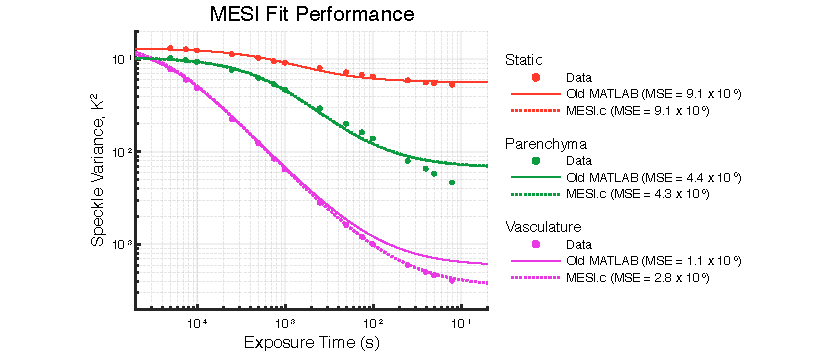
\includegraphics{figures/chapter_4/mesifit.pdf}
    \caption[Comparison of MESI parameter fitting performance for the old MATLAB processing script and the new compiled MESI.c program.]{
        \label{fig:mesifit}
        Comparison of MESI parameter fitting performance for the old MATLAB processing script and the new compiled MESI.c program. ROIs covering vasculature (pink), parenchyma (green), and static skull (red) were examined. (MSE = Mean Squared Error).
    }
\end{figure}



%%%%%%%%%%%%%%%%%%%%%%%%%%%%%%%%%%%%%%%%%%%%%%%%%%%%%%%%%%%%%%%%%%%%%%%%%%%%%%%
% Section 4.3 - In Vivo Demonstration of MESI
%%%%%%%%%%%%%%%%%%%%%%%%%%%%%%%%%%%%%%%%%%%%%%%%%%%%%%%%%%%%%%%%%%%%%%%%%%%%%%%
\section{\textit{In Vivo} Demonstration of MESI}

The upgraded system was tested \textit{in vivo} with anesthetized mice to demonstrate the MESI technique. Figure \ref{fig:mesidemo}A depicts the 15 speckle contrast images composing a single MESI frame, each acquired with different exposure times. The shorter exposures only reveal the flow of the large central vein while the longer exposures show increasing vascular detail. This highlights the sensitivity of an exposure time to only certain ranges of particle speeds and why multiple exposures covering a broad range of values are necessary to more robustly estimate $\tau_c$.

Figure \ref{fig:mesidemo}B depicts the resulting MESI ICT image calculated from the set of speckle contrast images using the process described in Section \ref{sec:mesi_fit}. Because of the large range of $\tau_c$ values, ICT images are typically displayed using a logarithmic scale. This image represents the best estimate of $\tau_c$ currently possible using the LSCI technique. Figure \ref{fig:mesidemo}C plots the speckle variance ($K^2$) of the highlighted vascular and parenchyma regions and their corresponding fits to Equation \ref{eq:mesi}. As $\tau_c$ decreases with increased scattering particle speed, the speckle variance curve shifts towards the left. It is important to sample as much of this curve as possible in order to properly estimate the particle dynamics. The measurements within the vessel would likely benefit from the addition of shorter exposure times since only four exposures (50, 75, 100, 250 $\mu$s) capture the linear portion of the curve.

% Figure - MESI In Vivo Demonstration
\begin{figure}
    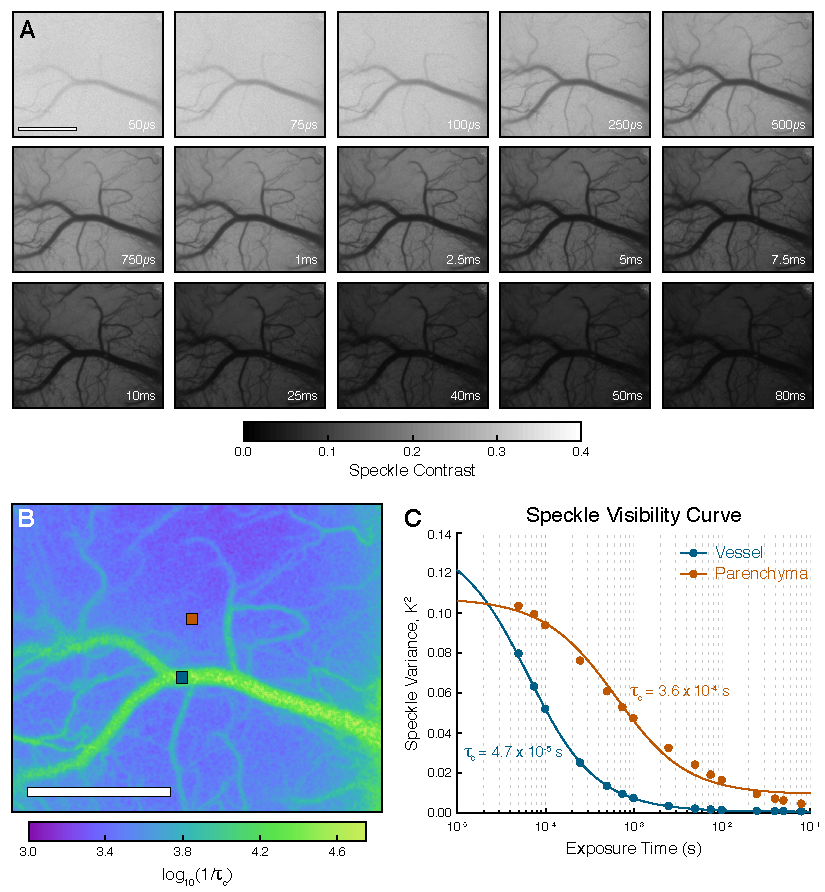
\includegraphics{figures/chapter_4/mesidemo.pdf}
    \caption{
        \label{fig:mesidemo}
        \textbf{(A)} Speckle contrast images from the mouse cortex for each of the 15 MESI exposures and \textbf{(B)} the resulting ICT image. \textbf{(C)} Fitted speckle variance ($K^2$) curves from the vascular (blue) and parenchyma (red) regions outlined in B. (Scale bars = 1 mm).
    }
\end{figure}



%%%%%%%%%%%%%%%%%%%%%%%%%%%%%%%%%%%%%%%%%%%%%%%%%%%%%%%%%%%%%%%%%%%%%%%%%%%%%%%
% Section 4.4 - Sensitivity and Reproducibility of MESI
%%%%%%%%%%%%%%%%%%%%%%%%%%%%%%%%%%%%%%%%%%%%%%%%%%%%%%%%%%%%%%%%%%%%%%%%%%%%%%%
\section{Sensitivity and Reproducibility of MESI}

Microfluidic devices have been used extensively to characterize both LSCI and MESI because they offer controlled testing environments with precise regulation of flow rates \cite{Parthasarathy:2008el, Richards:2013bi, Kazmi:2015du}. While syringe pumps are broadly utilized, they are prone to unwanted oscillations and frequently exhibit slow responsivity to flow changes \cite{Korczyk:2010eu, Zhou:2011ey, Li:2014ca}. Pressure-based flow regulation systems overcome the traditional mechanical limitations of syringe pumps by using air pressure to push fluids at a constant flow rate. Coupled with inline measurements of absolute flow for feedback, these systems allow for users to directly program complex flow profiles.

%%%%%%%%%%%%%%%%%%%%%%%%%%%%%%%%%%%%%%%%%%%%%%%%%%%%%%%%%%%%%%%%%%%%%%%%%%%%%%%
\subsection{Standalone MESI Instrumentation}

The microfluidic tests were performed on a standalone MESI system (Figure \ref{fig:standaloneschematic}) that features similar instrumentation to the previously described dual-modality imaging system. A 785 nm wavelength-stabilized laser diode (300 mW, LD785-SEV300, Thorlabs, Inc.) was mounted in a temperature-controlled housing (TCLDM9, Thorlabs, Inc.) and collimated using an aspheric lens (?, Thorlabs, Inc.). The operating current was set to 380 mA using a laser diode controller (LDC205C, Thorlabs, Inc.) and the diode temperature set to 25 $^\circ$C using a temperature controller (TED200C, Thorlabs, Inc.). The collimated laser light was passed through an optical isolator (?) to minimize back reflections that interfere with single frequency performance. Because the external volume holographic grating of the stabilized laser diode produces a dark spot in the far field, the laser was coupled into a X $\mu$ single mode fiber (?, Thorlabs, Inc.) to obtain a Gaussian beam. The fiber output was re-collimated and modulated using a 100 MHz AOM (3100-125 AOM + 1110AF-AIFO-1.0 RF Driver, Gooch \& Housego) with the first order diffraction isolated and relayed to obliquely illuminate the sample. A pair of camera lenses were used to image the scattered light (? , Nikon) with ?X magnification through a bandpass filter (?) to a CMOS camera (acA1920-155um, 1920 x 1200 pixels, Basler AG). Only a subset of the overall sensor array was used (? x ? pixels), resulting in a FOV of ? x ? mm. A multifunction I/O device (USB-6363, National Instruments Corp.) was used to produce the camera exposure trigger signals and AOM modulation voltages.

% Figure - Standalone MESI System Schematic
\begin{figure}
    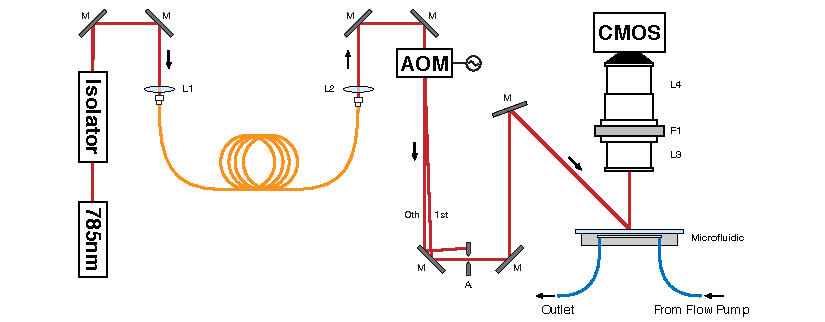
\includegraphics{figures/chapter_4/standaloneschematic.pdf}
    \caption{
        \label{fig:standaloneschematic}
        Schematic of the standalone MESI system used for microfluidic testing.
    }
\end{figure}

%%%%%%%%%%%%%%%%%%%%%%%%%%%%%%%%%%%%%%%%%%%%%%%%%%%%%%%%%%%%%%%%%%%%%%%%%%%%%%%
\subsection{Microfluidic Device}

The microfluidic device utilized for testing MESI featured a single 300 x 300 $\mu$m cross-sectional channel and was fabricated from polydimethylsiloxane (PDMS). 1.8 mg of titanium dioxide (\ce{TiO2}) was added per gram of PDMS to produce background scattering properties ($\mu_s$' = 8 cm$^{-1}$)\cite{Parthasarathy:2008el} similar to that of extravascular brain tissue for visible-NIR wavelengths of light \cite{Yaroslavsky:2002tg}. The complete manufacturing process can be found in \cite{Richards:2016hy}.

In order to measure the flow rate through the phantom, a mass flow sensor (Flow Sensor L, Fluigent Inc.) was placed in-line between the pressure-based flow control system and the inlet of the microfluidic device. The sensor was connected to a proprietary hub (FlowBoard, Fluigent Inc.) and the accompanying software (MAESFLO, Fluigent Inc.) used to record the absolute flow rate. The pressure control system (MFCS-EZ, Fluigent Inc.) was connected to the house air line via a 500 mbar regulator and a 15 mL pressurized reservoir (Fluiwell-1C, Fluigent Inc.) filled with the liquid used in the microfluidic. The flow rate control software was used to adjust air pressure to the reservoir in order to achieve the desired flow rate as measured with the flow sensor. This feedback mechanism allows the flow system to compensate for deviations caused by particle aggregation or air bubbles.

A suspension of 1 $\mu$m diameter polystyrene microspheres (5100A, Thermo Fisher Scientific) in ultra-filtered deionized water was utilized as a blood-mimicking sample. The microsphere concentration was selected to match to the scattering coefficient of whole blood ($\mu_s$ = 243 cm$^{-1}$) assuming a 50\% hematocrit and \ce{SO2} \textgreater 98\% \cite{Yaroslavsky:2002tg}. Prior to a microfluidic experiment, the solution was sonicated in a glass vial to fully suspend the particles and degassed under vacuum to remove any bubbles that could disrupt stable flow. Figure \ref{fig:microfluidic}A depicts a 5 ms LSCI frame of the 300 $\mu$m microfluidic channel with a flow rate of 10 mm/s. The highlighted ROI was used for all MESI ICT measurements. Figure \ref{fig:microfluidic}B depicts the stepped flow profile utilized in all the microfluidic experiments measured using the inline flow sensor. The flow rate is increased from 1-10 mm/s in 0.5 mm/s increments over the course of 40 minutes. This range of flow rates was selected based on prior measurements of red blood cell velocities in rodent microvasculature \cite{Tomita:2008do}.

% Figure - Microfluidic Image + Flow Profile
\begin{figure}
    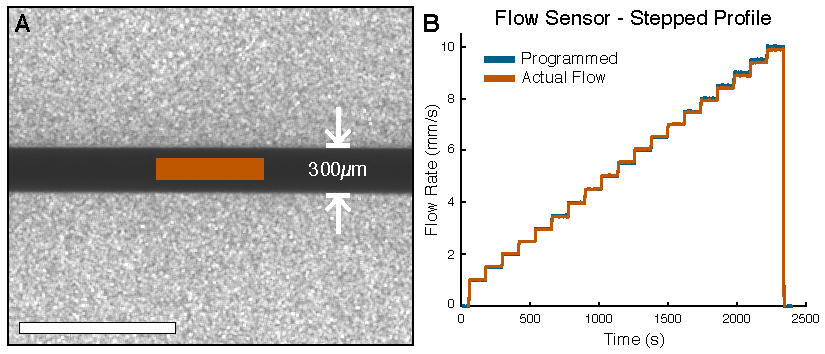
\includegraphics{figures/chapter_4/microfluidic.pdf}
    \caption{
        \label{fig:microfluidic}
        \textbf{(A)} Speckle contrast image of the 300 $\mu$m microfluidic channel (Scale bar = 1 mm). The highlighted ROI is used for all subsequent flow analyses. \textbf{(B)} Stepped flow profile measured using the inline flow sensor with flow rates ranging between 1-10 mm/s.
    }
\end{figure}

%%%%%%%%%%%%%%%%%%%%%%%%%%%%%%%%%%%%%%%%%%%%%%%%%%%%%%%%%%%%%%%%%%%%%%%%%%%%%%%
\subsection{Microfluidic Measurements with MESI}

MESI was used to continuously image the microfluidic channel over the duration of the 40-minute stepped flow profile with an acquisition rate of approximately 1.5 fps. The average speckle contrast was computed at each timepoint within the ROI highlighted in Figure \ref{fig:microfluidic}A. Because $\beta$ is theoretically a constant that only depends upon experimental conditions, it was estimated by performing an initial fit of the median of the data to Equation \ref{eq:mesi}. The full multi-exposure speckle contrast timecourse was then fit to the same equation while holding $\beta$ constant at the estimated value. A moving average filter ($n$ = 5) was applied to the resulting $\tau_c$ timecourse.

In order to compare the fitted values of $\tau_c$ to the absolute measurements from the flow sensor, the relative values of both measurements were computed using the 10 mm/s flow step as the baseline (Figure \ref{fig:microfluidicrelativeflow}A). The MESI rICT measurements closely mirror the flow sensor measurements with increased deviation at the slower flow rates and greater fluctuations over the entire flow profile. The measured speckle variance ($K^2$) and resulting MESI fits for each integer flow rate can be seen in Figure \ref{fig:microfluidicrelativeflow}B. The relationship between increasing flow rates and $\tau_c$ can be seen as the curves shift towards the left. Because $\beta$ was held constant, all the curves are converging to the same value (0.1430) as the exposure time approaches zero. However, this can negatively impact the quality of the resulting fits, as seen with the 1 mm/s curve, which deviates from the measured speckle variance at the shorter exposure times.

% Figure - Microfluidic Relative Flow
\begin{figure}
    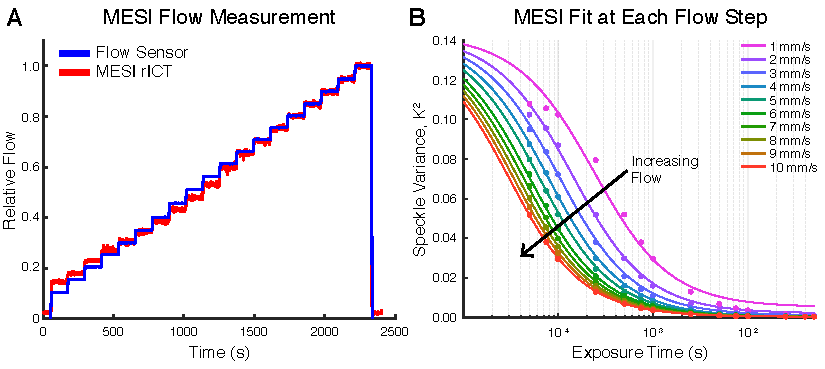
\includegraphics{figures/chapter_4/microfluidicrelativeflow.pdf}
    \caption{
        \label{fig:microfluidicrelativeflow}
        \textbf{(A)} Performance of MESI relative flow estimates compared to the flow sensor. Both measurements were normalized against the final 10 mm/s flow step. \textbf{(B)} Speckle variance curves and MESI fits from each flow step highlighting the relationship between flow rate and $\tau_c$.
    }
\end{figure}

The same measurements were conducted across multiple trials to examine the reproducibility of the MESI estimates of ICT (Figure \ref{fig:microfluidicconsistency}A). Runs 1 and 2 produced almost identical plots while Runs 3 and 4 appear to deviate at flow rates \textgreater 5 mm/s. However, plotting the average ICT against the average flow sensor measurements during each step (Figure \ref{fig:microfluidicconsistency}B) reveals that the flow system overshot the requested values during Runs 3 and 4. Therefore the apparent deviations in ICT seen in Figure \ref{fig:microfluidicconsistency}A were actually caused by the flow rate being higher during those two runs. These results indicate that MESI can provide stable day-to-day estimates of $\tau_c$ across a broad range of flow rates, thereby allowing the parameter to serve as a reliable baseline value for chronic or multiple-animal studies. The strong linear relationship between ICT and absolute flow rate suggests that calibrated measurements could be possible under ideal conditions.

% Figure - Microfluidic Consistency
\begin{figure}
    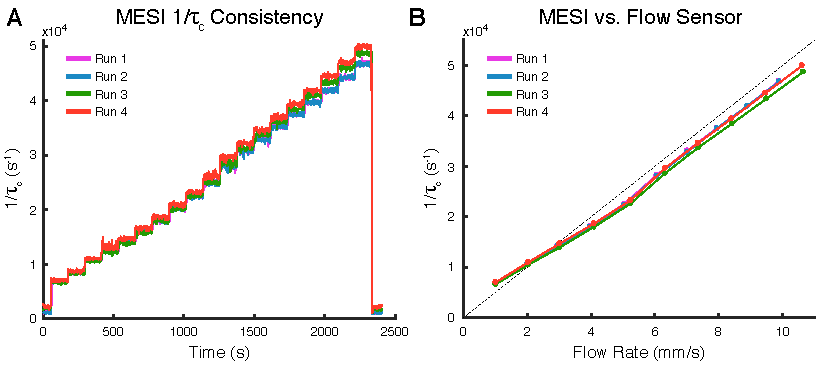
\includegraphics{figures/chapter_4/microfluidicconsistency.pdf}
    \caption{
        \label{fig:microfluidicconsistency}
        \textbf{(A)} Consistency of MESI ICT measurements across multiple trials. \textbf{(B)} MESI underestimates ICT at higher flow rates resulting in a slight divergence from unity. Error bars (s.d.) are displayed but smaller than the data markers.
    }
\end{figure}



%%%%%%%%%%%%%%%%%%%%%%%%%%%%%%%%%%%%%%%%%%%%%%%%%%%%%%%%%%%%%%%%%%%%%%%%%%%%%%%
% Section 4.5 - Discussion
%%%%%%%%%%%%%%%%%%%%%%%%%%%%%%%%%%%%%%%%%%%%%%%%%%%%%%%%%%%%%%%%%%%%%%%%%%%%%%%
\section{Discussion}

The MESI technique allows for more robust estimates of $\tau_c$ compared to traditional single-exposure LSCI \cite{Parthasarathy:2008el}. The improved mathematical model properly accounts for the presence of static scatterers in a sample and the multiple exposure times sample a broader range of flow rates. The implementation of MESI in the dual-modality imaging system facilitates more reliable measurements of flow deficits during targeted photothrombotic stroke \cite{Parthasarathy:2010vo} and improves the quantitative accuracy of chronic CBF measurements \cite{Kazmi:2013hp}. The upgraded system was demonstrated \textit{in vivo} by imaging the cortical vasculature of a mouse and examining the quality of the resulting MESI ICT imagery.

The modifications made to the Speckle Software, optimization of the calibration procedure, and improvements in processing speed have simplified the use of the MESI technique. Because the MATLAB script controlling the camera exposure trigger signals and AOM modulation voltages currently utilizes the ANSI C NI-DAQmx library, integrating the entire MESI calibration and acquisition process into the Speckle Software should be relatively straightforward. The \textgreater800x improvement in processing speed achieved with the compiled fitting program facilitates the full-frame analysis of MESI data that was previously impractical because of computation time. While still insufficient for the real-time processing of full-resolution speckle imagery, downsampling by a factor of two could allow for near 1 fps views of MESI-estimated ICT in the Speckle Software.

The microfluidic measurements conducted on the standalone MESI system further demonstrate the robustness of the technique for estimating $\tau_c$. The linear relationship between ICT and absolute flow rate highlights the broad range of flows that can be properly measured by MESI. The day-to-day stability of ICT estimates allow the metric to serve as a reliable baseline for chronic or multiple-animal studies. While the standalone system utilized an expensive wavelength-stabilized laser diode, any day-to-day fluctuations should be accounted for by the $\beta$ parameter in Equation \ref{eq:mesi} as long as the laser is not mode hopping. The optimization of the LSCI laser diode in the dual-modality system (Section \ref{ssec:laser_stability}) indicated stable speckle contrast measurements over time.



%%%%%%%%%%%%%%%%%%%%%%%%%%%%%%%%%%%%%%%%%%%%%%%%%%%%%%%%%%%%%%%%%%%%%%%%%%%%%%%
% END Chapter 4
%%%%%%%%%%%%%%%%%%%%%%%%%%%%%%%%%%%%%%%%%%%%%%%%%%%%%%%%%%%%%%%%%%%%%%%%%%%%%%%


% Chapter 5 - Chronic Awake Imaging of Photothrombotic Stroke
%%%%%%%%%%%%%%%%%%%%%%%%%%%%%%%%%%%%%%%%%%%%%%%%%%%%%%%%%%%%%%%%%%%%%%%%%%%%%%%
% Chapter 5 - Chronic Awake Imaging of Photothrombotic Stroke
%%%%%%%%%%%%%%%%%%%%%%%%%%%%%%%%%%%%%%%%%%%%%%%%%%%%%%%%%%%%%%%%%%%%%%%%%%%%%%%

\chapter{Chronic Awake Imaging of Photothrombotic Stroke} \label{Chapter_5}

\blindtext



%%%%%%%%%%%%%%%%%%%%%%%%%%%%%%%%%%%%%%%%%%%%%%%%%%%%%%%%%%%%%%%%%%%%%%%%%%%%%%%
% Section 5.1 - Awake Imaging System Designs
%%%%%%%%%%%%%%%%%%%%%%%%%%%%%%%%%%%%%%%%%%%%%%%%%%%%%%%%%%%%%%%%%%%%%%%%%%%%%%%
\section{Awake Imaging System Designs}

\blindtext



%%%%%%%%%%%%%%%%%%%%%%%%%%%%%%%%%%%%%%%%%%%%%%%%%%%%%%%%%%%%%%%%%%%%%%%%%%%%%%%
% Section 5.2 - Awake vs. Anesthetized Measurements
%%%%%%%%%%%%%%%%%%%%%%%%%%%%%%%%%%%%%%%%%%%%%%%%%%%%%%%%%%%%%%%%%%%%%%%%%%%%%%%
\section{Improving MESI Processing Speed}

\blindtext



%%%%%%%%%%%%%%%%%%%%%%%%%%%%%%%%%%%%%%%%%%%%%%%%%%%%%%%%%%%%%%%%%%%%%%%%%%%%%%%
% Section 5.3 - Awake Targeted Photothrombosis Induction
%%%%%%%%%%%%%%%%%%%%%%%%%%%%%%%%%%%%%%%%%%%%%%%%%%%%%%%%%%%%%%%%%%%%%%%%%%%%%%%
\section{Awake Targeted Photothrombosis Induction}

\blindtext



%%%%%%%%%%%%%%%%%%%%%%%%%%%%%%%%%%%%%%%%%%%%%%%%%%%%%%%%%%%%%%%%%%%%%%%%%%%%%%%
% Section 5.4 - Chronic Awake Post-Stroke Hemodynamics
%%%%%%%%%%%%%%%%%%%%%%%%%%%%%%%%%%%%%%%%%%%%%%%%%%%%%%%%%%%%%%%%%%%%%%%%%%%%%%%
\section{Chronic Awake Post-Stroke Hemodynamics}

\blindtext



%%%%%%%%%%%%%%%%%%%%%%%%%%%%%%%%%%%%%%%%%%%%%%%%%%%%%%%%%%%%%%%%%%%%%%%%%%%%%%%
% Section 5.5 - Discussion
%%%%%%%%%%%%%%%%%%%%%%%%%%%%%%%%%%%%%%%%%%%%%%%%%%%%%%%%%%%%%%%%%%%%%%%%%%%%%%%
\section{Discussion}

\blindtext



%%%%%%%%%%%%%%%%%%%%%%%%%%%%%%%%%%%%%%%%%%%%%%%%%%%%%%%%%%%%%%%%%%%%%%%%%%%%%%%
% END Chapter 5
%%%%%%%%%%%%%%%%%%%%%%%%%%%%%%%%%%%%%%%%%%%%%%%%%%%%%%%%%%%%%%%%%%%%%%%%%%%%%%%


% Chapter 6 - Conclusions
%%%%%%%%%%%%%%%%%%%%%%%%%%%%%%%%%%%%%%%%%%%%%%%%%%%%%%%%%%%%%%%%%%%%%%%%%%%%%%%
% Chapter 6 - Conclusions
%%%%%%%%%%%%%%%%%%%%%%%%%%%%%%%%%%%%%%%%%%%%%%%%%%%%%%%%%%%%%%%%%%%%%%%%%%%%%%%

\chapter{Conclusions} \label{Chapter_6}

\blindtext



%%%%%%%%%%%%%%%%%%%%%%%%%%%%%%%%%%%%%%%%%%%%%%%%%%%%%%%%%%%%%%%%%%%%%%%%%%%%%%%
% Section 6.1 - Future Work
%%%%%%%%%%%%%%%%%%%%%%%%%%%%%%%%%%%%%%%%%%%%%%%%%%%%%%%%%%%%%%%%%%%%%%%%%%%%%%%
\section{Future Work}

\blindtext



%%%%%%%%%%%%%%%%%%%%%%%%%%%%%%%%%%%%%%%%%%%%%%%%%%%%%%%%%%%%%%%%%%%%%%%%%%%%%%%
% END Chapter 6
%%%%%%%%%%%%%%%%%%%%%%%%%%%%%%%%%%%%%%%%%%%%%%%%%%%%%%%%%%%%%%%%%%%%%%%%%%%%%%%



%%%%%%%%%%%%%%%%%%%%%%%%%%%%%%%%%%%%%%%%%%%%%%%%%%%%%%%%%%%%%%%%%%%%%%
% Appendices
%%%%%%%%%%%%%%%%%%%%%%%%%%%%%%%%%%%%%%%%%%%%%%%%%%%%%%%%%%%%%%%%%%%%%%
\appendices

% Appendix A - Derivation of the Stern-Volmer Relationship
%%%%%%%%%%%%%%%%%%%%%%%%%%%%%%%%%%%%%%%%%%%%%%%%%%%%%%%%%%%%%%%%%%%%%%%%%%%%%%%
% Appendix A - Derivation of the Stern-Volmer Relationship
%%%%%%%%%%%%%%%%%%%%%%%%%%%%%%%%%%%%%%%%%%%%%%%%%%%%%%%%%%%%%%%%%%%%%%%%%%%%%%%

\chapter{Derivation of the Stern-Volmer Relationship}

Upon absorption of radiation, a phosphorescent molecule is excited from its singlet ground state ($S_0$) to an excited singlet state ($S_1$) while maintaining the pairing of its electron spins. The excited singlet state can then non-radiatively transition to an excited triplet state ($T_1$) through a process known as intersystem crossing. This results in the unpairing of its ground and excited state electron spins.

The excited triplet state molecule can return back to its singlet ground state through either radiative or non-radiative relaxation. The radiative relaxation from the excited triplet state to the singlet ground state is known as phosphorescence and occurs with a decay rate $k_{r}$. Non-radiative relaxation occurs through intersystem crossing at a decay rate $k_{n-r}$. Collision with ground triplet state molecular oxygen (\ce{^3O2}) can quench the excited triplet state molecule back to its singlet ground state while producing excited singlet state oxygen (\ce{^1O2}). This transfer of electronic excitation energy can be modeled as a first order reaction with a decay rate proportional to the product of the quenching constant ($k_{q}$) and the concentration of dissolved oxygen ([\ce{O2}]).
%
The overall rate equation can be expressed as:
%
\begin{equation}
    \frac{d[P^*]}{dt} = -(k_{r} + k_{n-r} + k_{q}[O_{2}])[P^{*}]
\end{equation}
%
where $[P^{*}]$ denotes the number of excited triplet state molecules. Assuming that $[O_{2}] >> [P^{*}]$, then the rate equation can be integrated to:
%
\begin{equation}
    [P^*] = -[P^{*}]_{0}e^{-(k_{r} + k_{n-r} + k_{q}[O_{2}])t}
\end{equation}
%
The lifetime in the presence of the quencher ($\tau$) can then be defined by inversion of the overall decay rate:
%
\begin{equation}
    \tau = \frac{1}{k_{r} + k_{n-r} + k_{q}[O_{2}]}
\end{equation}
%
In the absence of the quencher ($[O_2] = 0$), the lifetime can be simplified to:
%
\begin{equation}
    \tau_{0} = \frac{1}{k_{r} + k_{n-r}}
\end{equation}
%
and used to normalize the lifetime in the presence of the quencher:
%
\begin{equation}
    \frac{\tau_{0}}{\tau} = \frac{k_{r} + k_{n-r} + k_{q}[O_{2}]}{k_{r} + k_{n-r}}
\end{equation}
%
This can be simplified to a linear expression known as the Stern-Volmer Relationship:
%
\begin{equation}
    \frac{\tau_{0}}{\tau} = 1 + k_{q}\tau_{0}[O_{2}]
\end{equation}
%
Using Henry's Law for dissolved gases at the sample temperature, the molecular oxygen concentration [\ce{O2}] can be related to the partial pressure of oxygen (\ce{pO2}) as follows:
%
\begin{equation}
    \begin{split}
        \frac{\tau_{0}}{\tau} & = 1 + k_{q}\tau_{0}K_{H}[O_{2}] \\
        & = 1 + k_{q}\tau_{0}[pO_{2}]
    \end{split}
\end{equation}
%
Lifetime can also be calibrated against a standard that quantifies either the [\ce{O2}] or \ce{pO2} in a solution that matches the pH, atmospheric pressure, temperature, and salinity of the desired sample environment.


% Appendix B - Accessing the DMD on the DLP LightCrafter
%%%%%%%%%%%%%%%%%%%%%%%%%%%%%%%%%%%%%%%%%%%%%%%%%%%%%%%%%%%%%%%%%%%%%%%%%%%%%%%
% Appendix B - Accessing the DMD on the DLP LightCrafter
%%%%%%%%%%%%%%%%%%%%%%%%%%%%%%%%%%%%%%%%%%%%%%%%%%%%%%%%%%%%%%%%%%%%%%%%%%%%%%%

\chapter{Accessing the DMD on the DLP LightCrafter}

The Texas Instruments DLP LightCrafter evaluation module contains a DLP3000 DMD, a DM365 embedded processor running Linux, and an RGB LED light engine developed by Young Optics (Figure \ref{fig:dmd_mod_0}). In order to utilize a custom light source such as a laser, the light engine must be removed to gain physical access to the DMD. The following series of figures details the disassembly process necessary to access and remount the DMD for use with custom illumination.

% Figure - LightCrafter Overview
\begin{figure}
    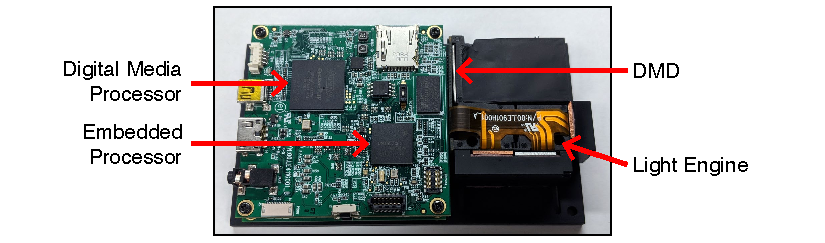
\includegraphics{figures/appendix_b/dmd_mod_0.pdf}
    \caption {
        \label{fig:dmd_mod_0}
        Overview of the Texas Instruments DLP LightCrafter.
    }
\end{figure}

Remove the four screws (Phillips head) on the top of device and detach the upper circuit board from the lower half of the device (Figure \ref{fig:dmd_mod_1}). Turn the device upside down and remove the four screws (Phillips head) attaching the light engine to the baseplate from the bottom (Figure \ref{fig:dmd_mod_2}). Flip the device back over and remove the three screws (Phillips head) attaching the light engine from the top. Remove the two screws (Phillips head) horizontally securing the light engine to the circuit board (Figure \ref{fig:dmd_mod_3}). Use a flat-head screwdriver to flip the locking clips on the two ribbon cables connecting the light engine to the circuit board and disconnect the cables.

% Figure - LightCrafter Modification: Step 1
\begin{figure}
    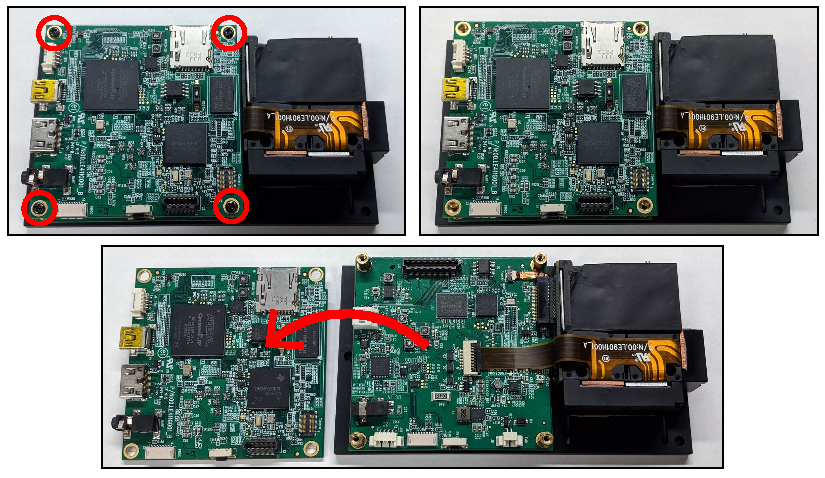
\includegraphics{figures/appendix_b/dmd_mod_1.pdf}
    \caption {
        \label{fig:dmd_mod_1}
        Detach the upper circuit board from the device.
    }
\end{figure}

% Figure - LightCrafter Modification: Step 2
\begin{figure}
    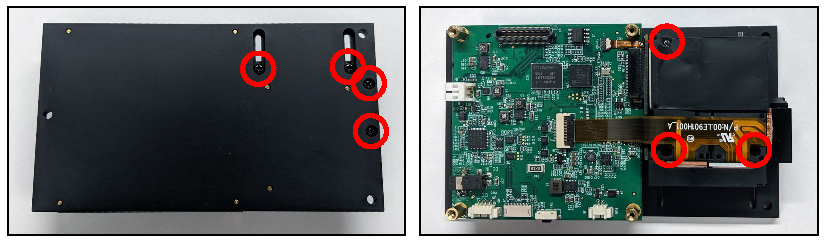
\includegraphics{figures/appendix_b/dmd_mod_2.pdf}
    \caption {
        \label{fig:dmd_mod_2}
        Remove the screws attaching the light engine to the baseplate.
    }
\end{figure}

% Figure - LightCrafter Modification: Step 3
\begin{figure}
    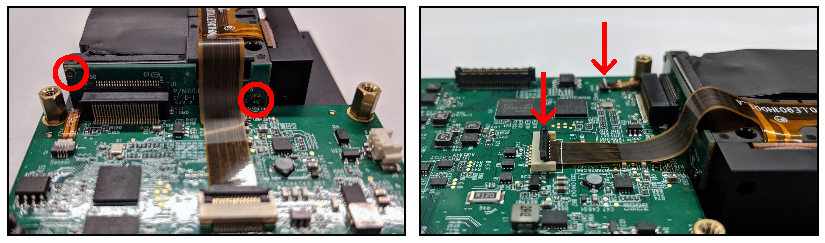
\includegraphics{figures/appendix_b/dmd_mod_3.pdf}
    \caption {
        \label{fig:dmd_mod_3}
        Remove the screws and ribbon cables connecting the light engine to the circuit board.
    }
\end{figure}

At this point, the only physical connection remaining between the light engine and the rest of the device is through the DMD mounting socket. Remove the entire light engine by pulling horizontally and slightly upwards to disconnect the DMD (Figure \ref{fig:dmd_mod_4}). Remove the two screws (Phillips head) on the plate securing the DMD in the light engine (Figure \ref{fig:dmd_mod_5}). Remove the metal plate and extract the DMD chip.

% Figure - LightCrafter Modification: Step 4
\begin{figure}
    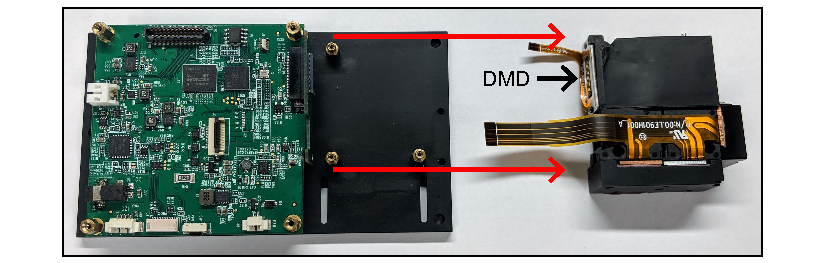
\includegraphics{figures/appendix_b/dmd_mod_4.pdf}
    \caption {
        \label{fig:dmd_mod_4}
        Disconnect the light engine from the board.
    }
\end{figure}

% Figure - LightCrafter Modification: Step 5
\begin{figure}
    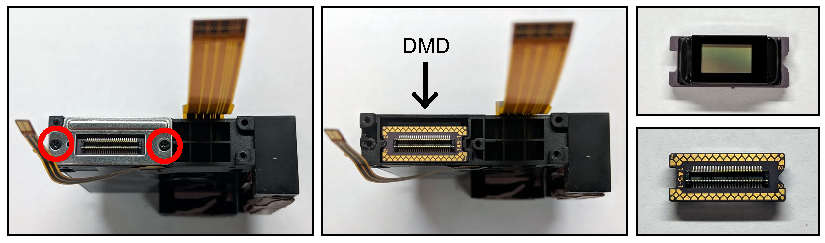
\includegraphics{figures/appendix_b/dmd_mod_5.pdf}
    \caption {
        \label{fig:dmd_mod_5}
        Extract the DMD from the light engine.
    }
\end{figure}

In order to improve physical access to the DMD, the bottom board can be reoriented on the baseplate. Remove the four standoff screws and rotate the bottom board by 180$^\circ$ so that the DMD mounting socket is facing outwards (Figure \ref{fig:dmd_mod_6}). Any modifications to the baseplate (e.g. drilling holes for mounting) should be performed at this stage since all electronics are currently detached. Reattach the bottom circuit board to the baseplate using the standoff screws and reconnect the DMD to its mounting socket. The notch, which indicates the illumination orientation, should be facing towards the right. Reattach the top circuit board and secure with the four screws removed at the beginning.

% Figure - LightCrafter Modification: Step 6
\begin{figure}
    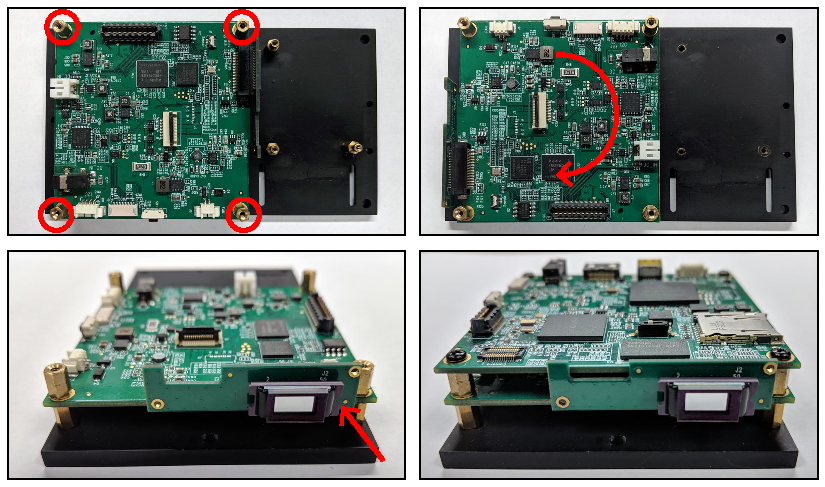
\includegraphics{figures/appendix_b/dmd_mod_6.pdf}
    \caption {
        \label{fig:dmd_mod_6}
        Rotate the bottom circuit board by 180$^\circ$, reconnect the DMD to its socket, and reattach the upper circuit board.
    }
\end{figure}

The LightCrafter is now configured for use with custom illumination paradigms such as the one described in this dissertation. Because the DMD is exposed on the edge of the device, care should be taken to avoid physical contact that might damage the device.



%%%%%%%%%%%%%%%%%%%%%%%%%%%%%%%%%%%%%%%%%%%%%%%%%%%%%%%%%%%%%%%%%%%%%%%%%%%%%%%
% END Appendix B
%%%%%%%%%%%%%%%%%%%%%%%%%%%%%%%%%%%%%%%%%%%%%%%%%%%%%%%%%%%%%%%%%%%%%%%%%%%%%%%


% Appendix C - Sterile Cranial Window Surgical Preparation
%%%%%%%%%%%%%%%%%%%%%%%%%%%%%%%%%%%%%%%%%%%%%%%%%%%%%%%%%%%%%%%%%%%%%%%%%%%%%%%
% Appendix C - Sterile Cranial Window Surgical Preparation
%%%%%%%%%%%%%%%%%%%%%%%%%%%%%%%%%%%%%%%%%%%%%%%%%%%%%%%%%%%%%%%%%%%%%%%%%%%%%%%

\chapter{Sterile Cranial Window Surgical Preparation} \label{app:cranial_window}

While the optical imaging techniques described in this dissertation are non-contact, a chronic cranial window implantation is required to obtain optical access to brain tissue. This appendix details the craniotomy procedure and maintenance protocol utilized for chronic \textit{in vivo} awake imaging in mice. All animal protocols were approved by the Institutional Animal Care and Use Committee at The University of Texas at Austin.


%%%%%%%%%%%%%%%%%%%%%%%%%%%%%%%%%%%%%%%%%%%%%%%%%%%%%%%%%%%%%%%%%%%%%%%%%%%%%%%
% Section B.1 - Implantation of Cranial Window
%%%%%%%%%%%%%%%%%%%%%%%%%%%%%%%%%%%%%%%%%%%%%%%%%%%%%%%%%%%%%%%%%%%%%%%%%%%%%%%
\section{Implantation of Cranial Window}

Mice (CD-1, male, 25-30 g, Charles River) were anesthetized with medical air vaporized isoflurane (2.0\%) via nose-cone inhalation. Body temperature was maintained at 37 $^\circ$C with a feedback heating pad (DC Temperature Controller, FHC). Arterial oxygen saturation, heart rate, and breath rate were monitored via pulse oximetry (MouseOx, Starr Life Sciences). After induction, mice were placed supine in a head-fixed stereotaxic frame (Narishige Scientific Instrument Lab) and administered carprofen (5 mg/kg, subcutaneous) for anti-inflammation and dexamethasone (2 mg/kg, intramuscular) to reduce the severity of cerebral edema following removal of the skull. Surgical instruments and artificial cerebrospinal fluid (ACSF, buffered pH 7.4) used during the craniotomy procedure were sterilized in an autoclave.

% Figure - Cranial Window Location
\begin{figure}
    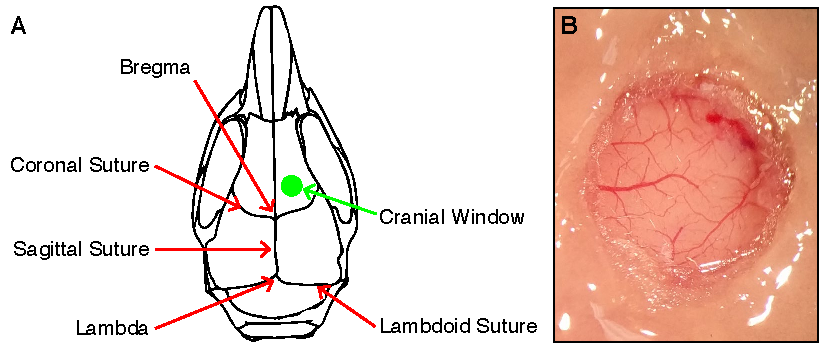
\includegraphics{figures/appendix_c/cranialwindow.pdf}
    \caption[Location of the cranial window on the mouse skull]{
        \label{fig:cranialwindow}
        Location of the cranial window relative to bregma. Skull illustratrion adapted from \cite{Cook:1965wb}.
    }
\end{figure}

The scalp was shaved and resected to expose skull between the bregma and lambda cranial coordinates. A thin layer of cyanoacrylate (Vetbond Tissue Adhesive, 3M) was applied to the exposed skull to facilitate the adhesion of dental cement during a later step. A 2-3 mm diameter portion of the skull over the frontoparietal cortex was removed while leaving the dura intact using a dental drill (0.8 mm burr, Ideal Microdrill, Fine Science Tools) with regular ACSF perfusion to prevent overheating. A 5 mm round cover glass (\#1.5, World Precision Instruments) was placed over the exposed brain and a dental cement mixture was deposited along the perimeter while applying gentle pressure to the cover glass. This process bonded the cover glass to the surrounding skull to create a sterile, air-tight seal around the craniotomy and allowed for restoration of intracranial pressure. A second layer of cyanoacrylate was applied over the dental cement to further seal the cranial window. The medial and anterior edges of the window were approximately 2 mm rostral from bregma and 0.5 mm lateral from the sagittal suture (Figure \ref{fig:cranialwindow}). Animals were allowed to recover from anesthesia and monitored for cranial window integrity and normal behavior for at least two weeks prior to imaging. Additional carprofen injections (5 mg/kg) were administered subcutaneously two, four, and seven days post-surgery to relieve inflammation from the procedure.


%%%%%%%%%%%%%%%%%%%%%%%%%%%%%%%%%%%%%%%%%%%%%%%%%%%%%%%%%%%%%%%%%%%%%%%%%%%%%%%
% Section B.2 - Headbar Attachment
%%%%%%%%%%%%%%%%%%%%%%%%%%%%%%%%%%%%%%%%%%%%%%%%%%%%%%%%%%%%%%%%%%%%%%%%%%%%%%%
\section{Headbar Attachment} \label{app:headbar_attachment}

Animals designated for awake imaging underwent an additional procedure during the application of dental cement to permanently attach a metal headbar used for head fixation. The circular cutout in the headbar was aligned with the cranial window and rotated laterally until parallel with the cover glass. This ensured that the cranial window would be perpendicular to the imaging system's optical axis when the animal was restrained in the awake imaging setup. Dental cement was applied around the headbar to permanently attach it to the animal's skull.


%%%%%%%%%%%%%%%%%%%%%%%%%%%%%%%%%%%%%%%%%%%%%%%%%%%%%%%%%%%%%%%%%%%%%%%%%%%%%%%
% Section B.3 - Chronic Animal Maintenance
%%%%%%%%%%%%%%%%%%%%%%%%%%%%%%%%%%%%%%%%%%%%%%%%%%%%%%%%%%%%%%%%%%%%%%%%%%%%%%%
\section{Chronic Animal Maintenance}

Animals were checked daily to monitor both behavior and the integrity of the cranial window by veterinary staff at the University of Texas at Austin Animal Research Center (ARC). Animals were housed in climate-controlled rooms with timed lighting (12-hour light/dark cycles) to maintain a comfortable living environment and given food and water \textit{ad libitum}. Social housing with multiple animals reduced the risk of overeating commonly seen when solo housing animals. This minimized possible growth in the animal's size and helped maintain the integrity of the cranial window. Any aggression resulted in the removal of the aggressor into a separate cage.

After several weeks of recovery, animals were used for both acute and chronic imaging experiments. Cranial windows were lightly cleaned prior to each imaging session using a cotton swab and 70\% ethanol (v/v). If necessary, a topical application of mineral oil was used to improve image quality by index matching. Any discoloration on or around the cranial window was documented and monitored for possible infection. Any cracks in or breaking of the cranial window were also documented and resulted in the immediate euthanasia of the animal.


%%%%%%%%%%%%%%%%%%%%%%%%%%%%%%%%%%%%%%%%%%%%%%%%%%%%%%%%%%%%%%%%%%%%%%%%%%%%%%%
% END Appendix B
%%%%%%%%%%%%%%%%%%%%%%%%%%%%%%%%%%%%%%%%%%%%%%%%%%%%%%%%%%%%%%%%%%%%%%%%%%%%%%%


% Appendix D - Jacobian Matrix of the MESI Equation
%%%%%%%%%%%%%%%%%%%%%%%%%%%%%%%%%%%%%%%%%%%%%%%%%%%%%%%%%%%%%%%%%%%%%%%%%%%%%%%
% Appendix D - Jacobian Matrix of the MESI Equation
%%%%%%%%%%%%%%%%%%%%%%%%%%%%%%%%%%%%%%%%%%%%%%%%%%%%%%%%%%%%%%%%%%%%%%%%%%%%%%%

\chapter{Jacobian Matrix of the MESI Equation}

The Jacobian matrix ($\bm{J}$) is the matrix of all first-order partial derivatives of a vector-valued function ($\bm{f}$):

\begin{equation}
    \bm{J} = \left[\frac{\partial \bm{f}}{\partial x_1} \ldots \frac{\partial \bm{f}}{\partial x_n}\right]
\end{equation}



%%%%%%%%%%%%%%%%%%%%%%%%%%%%%%%%%%%%%%%%%%%%%%%%%%%%%%%%%%%%%%%%%%%%%%
% Bibliography
%%%%%%%%%%%%%%%%%%%%%%%%%%%%%%%%%%%%%%%%%%%%%%%%%%%%%%%%%%%%%%%%%%%%%%
\bibliographystyle{unsrt}
\bibliography{bibliography.bib}


%%%%%%%%%%%%%%%%%%%%%%%%%%%%%%%%%%%%%%%%%%%%%%%%%%%%%%%%%%%%%%%%%%%%%%
% Vita
%%%%%%%%%%%%%%%%%%%%%%%%%%%%%%%%%%%%%%%%%%%%%%%%%%%%%%%%%%%%%%%%%%%%%%
\begin{vita}
\noindent Colin Tan Sullender was born in Birmingham, Alabama in 1988 to Wayne Sullender and Thuan Hong Tan. He graduated from Homewood High School in Homewood, Alabama in 2007. He pursued a Bachelor of Science in bioengineering at the University of Washington in Seattle and graduated in 2011 with College Honors in Bioengineering. As an undergraduate, he worked as a research assistant in the laboratory of Dr. Wendy E. Thomas. He began his doctorate in biomedical engineering at The University of Texas at Austin in 2011 in the laboratory of Dr. Andrew K. Dunn working on the development of novel optical imaging systems for studying ischemic stroke. He completed his Master of Science in Engineering in biomedical engineering in 2016 and completed his doctoral degree in December 2018.
\\
\\
Email Address: csullender@utexas.edu
\\
\\
This dissertation was typeset with \LaTeX{} by the author.
\end{vita}


%%%%%%%%%%%%%%%%%%%%%%%%%%%%%%%%%%%%%%%%%%%%%%%%%%%%%%%%%%%%%%%%%%%%%%
% END DOCUMENT
%%%%%%%%%%%%%%%%%%%%%%%%%%%%%%%%%%%%%%%%%%%%%%%%%%%%%%%%%%%%%%%%%%%%%%
\end{document}
